\documentclass[11pt, oneside, a4paper]{gsm-l}

%\usepackage[paperwidth=18cm,paperheight=24cm,margin=3cm]{geometry}

\usepackage{lymber}

\usepackage[T1]{fontenc}
\usepackage{textcomp}
\usepackage{mathpazo}
\usepackage{utopia}

\usepackage{makeidx}
\usepackage{tikz}
\usetikzlibrary{arrows,calc}
\usepackage{subfigure}

%\usepackage{preambulo}
%\usepackage[a4,center]{crop}	%sem marcas de corte
%\usepackage{microtype}
%\usepackage[normalem]{ulem}

%\graphicspath{./figuras/}

%%somatoria de i (troca o indice), ex: \Soma[j]{a_j}
%\newcommand{\SomaR}[2][i]{\sum\limits_{#1} {#2}}

%\newcommand{\rot}{\operatorname{rot}}	%rotacional

%\fancyfoot[LO,RE]{R\'egis {\Large \smiley} 2008}
%\fancyfoot[C]{\scriptsize{Curso de Ver\~ao IME USP 2008}}
%*******************************************************
\title{Cálculo no $\R^n$ \\ Curso de Verão 2008 -- IME - USP}
\author{Prof. Alexandre Lymberopoulos\\ Digitação: Régis da Silva Santos}
%*******************************************************

\makeindex

\begin{document}
% capa
% \thispagestyle{empty}
% \begin{tikzpicture}[remember picture,overlay,inner sep=0pt]
%   \node[above right] at (current page.south west) {
%       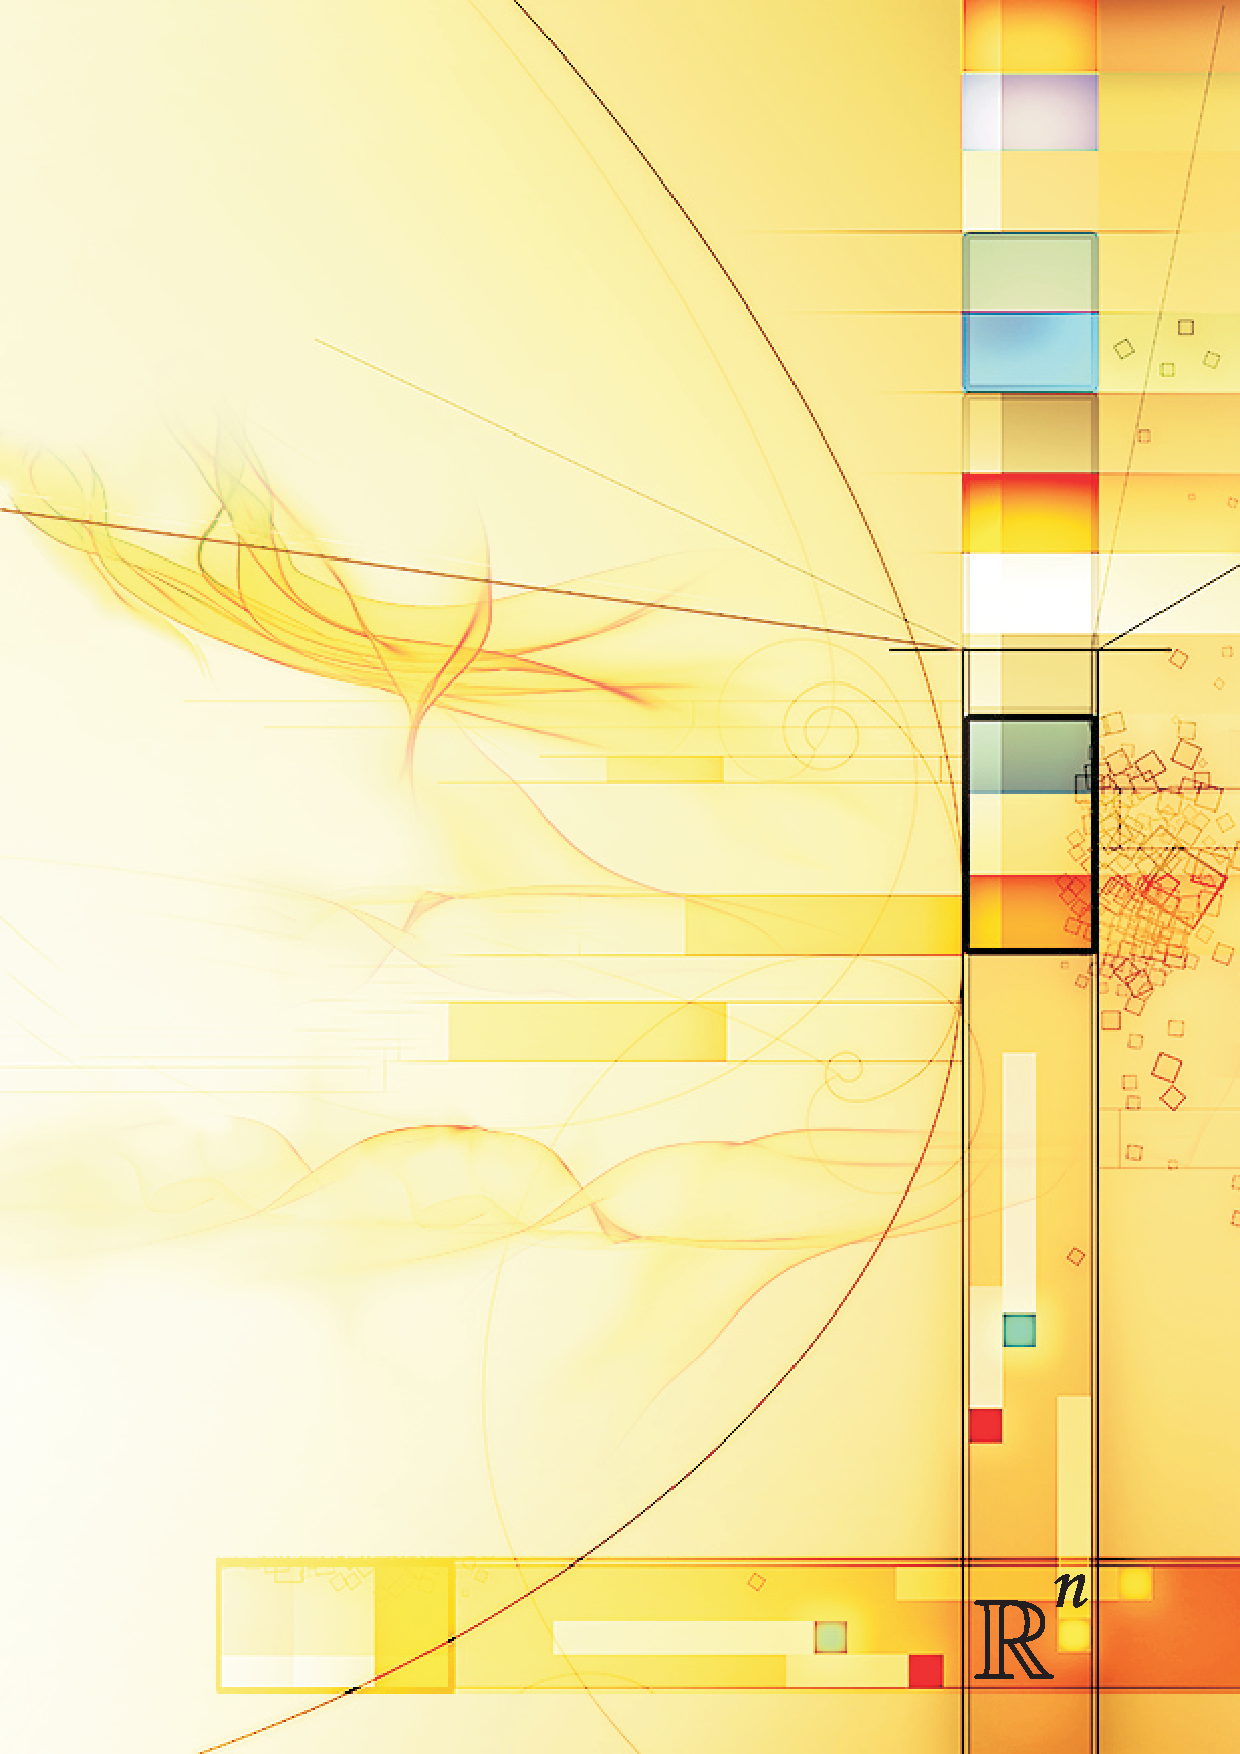
\includegraphics[width=210mm]{./capa/capa}
%   };
% \end{tikzpicture}
%*******************************************************

% \pagestyle{fancy}
\frontmatter

\maketitle

%*******************************************************
\chapter*{Prefácio}

Escrever um prefácio mais preciso contendo informações sobre o curso,
organização do texto, licenças para distribuição, autorias e digitações
etc.

% Este material foi criado a partir de notas de aula do Curso de Verão 2008 no IME-USP.

% É permitida a reprodução total ou parcial deste material desde que indicada a autoria.

% Este material foi criado para uso pessoal, portanto, adaptado para tal
% fim, podendo posteriormente ser adaptado para uso coletivo. E est\'a
% sujeito a conter erros, portanto, são aceitas sugest\~oes e cr\'iticas
% construtivas para melhoria do mesmo. 

% \vfill

% \begin{flushright}
% \textit{R\'egis da Silva Santos}

% Março de 2008.
% \end{flushright}
%*****************************************

\tableofcontents
\listoffigures

\mainmatter
% \pagestyle{fancy}

\chapter{Revisão de Cálculo}\label{revcalc}

\begin{defi}
  Uma \emph{bola aberta}\index{Bola aberta} de centro $x_0$ e raio $r$ é
  o conjunto \[B_r(x_0)=\big\{x\in\R:|x-x_0|<r\big\}.\]
  \begin{figure}[h]
    \centering
    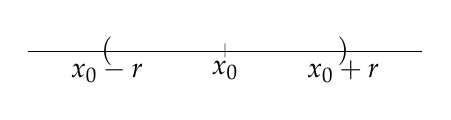
\begin{tikzpicture}
  \draw (0,0) -- (5,0);
  \node at (1,0) {$($};
  \node[below] at (1,0) {$x_0 - r$};
  \node at (4,0) {$)$};
  \node[below] at (4,0) {$x_0 + r$};
  \node at (2.5,0) {\tiny $|$};
  \node[below] at (2.5,0) {$x_0$};
\end{tikzpicture}

    \caption{Bola aberta em \R}
    \label{fig:bolaaberta}
  \end{figure}
%  \tkzfig{fig01}{Bola aberta}
\end{defi}

Seja $S$ um conjunto contido no domínio de $f$. Denotaremos por $f(S)$ a
imagem de $S$ pela função $f$, ou seja, $f(S)=\big\{f(x): x\in
S\big\}$. A fim de simplificar nomenclatura indicaremos uma bola aberta
simplesmente por bola.

\section{Continuidade}\label{revcalc:cont}
\begin{defi}
  Seja $f$ uma função. Dizemos que $f$ é
  \emph{contínua}\index{Função!contínua} em $x_0$ se para toda bola $F$,
  centrada em $f(x_0)$, existe $B$, bola centrada em $x_0$, tal que
  $f(B)\subset F$.
\end{defi}

\begin{figure}[!h]
  \centering
  \subfigure[Função contínua]{
    \usetikzlibrary{arrows,calc}
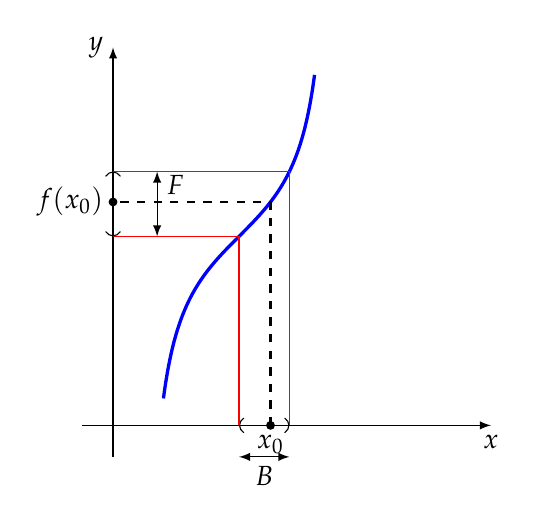
\begin{tikzpicture}[>=latex,scale=.8]
	%eixos
    \draw[->] (-.5,0) -- (6,0) node[below] {$x$};
    \draw[->] (0,-.5) -- (0,6) node[left] {$y$};
	%cotas
% 	\foreach \x in {1,...,5}
% 		\draw[shift={(\x,0)}] (0pt,2pt) -- (0pt,-2pt)
% 			node[below] 	{\footnotesize $\x$};
% 	\foreach \y in {1,...,5}
% 	\draw[shift={(0,\y)}] (2pt,0pt) -- (-2pt,0pt)
% 		node[left] {\footnotesize $\y$};
% 	\node[below left] at (0,0) {\footnotesize $0$};
	%grafico tan(x-2)+3
	\draw[blue,very thick,smooth,samples=100,domain=.8:3.2]
  plot(\x,{sin(\x r - 2 r)/cos(\x r - 2 r) + 3});
	%rotulo e intervalo do eixo Ox
	\draw[(-)] (2,0) -- (2.8,0);
	\fill (2.5,0) circle (2pt) node [below] {$x_0$};
	\draw[<->] (2,-.5) -- node[below] {$B$} (2.8,-.5);
	%faixas
	\draw[red] (2,0) -- (2,{sin(2 r - 2 r)/cos(2 r - 2 r) + 3}) -- (2,{sin(2 r - 2 r)/cos(2 r - 2 r) + 3} -| 0,0) coordinate (B2);
	\draw[red] (2.8,0) -- (2.8,{sin(2.8 r - 2 r)/cos(2.8 r - 2 r) + 3}) -- (2.8,{sin(2.8 r - 2 r)/cos(2.8 r - 2 r) + 3} -| 0,0) coordinate (B3);
	\draw[dashed,thick] (2.5,0) -- (2.5,{sin(2.5 r - 2 r)/cos(2.5 r - 2 r) + 3}) -- (2.5,{sin(2.5 r - 2 r)/cos(2.5 r - 2 r) + 3} -| 0,0) coordinate (F);
	%rotulo e intervalo do eixo Oy
	\draw[(-)] (B2) -- (B3);
	\fill (F) circle (2pt) node [left] {$f(x_0)$};
	\draw[<->] ($(B2) + (.7,0)$) -- node[above right] {$F$} ($(B3) + (.7,0)$);
\end{tikzpicture}
\label{funccont}}
  \subfigure[Função descontínua]{
    \usetikzlibrary{arrows,calc}
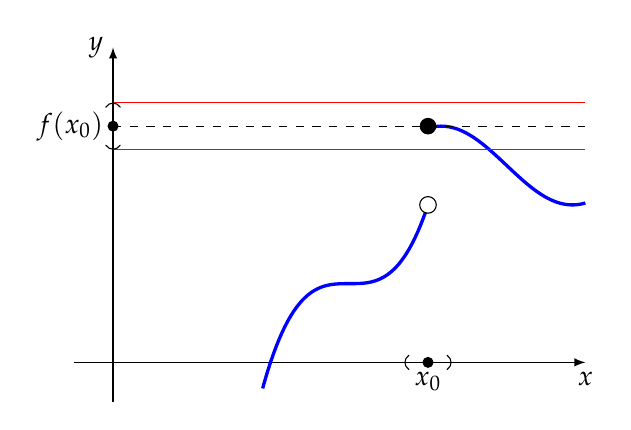
\begin{tikzpicture}[>=latex]
	%eixos
    \draw[->] (-.5,0) -- (6,0) node[below] {$x$};
    \draw[->] (0,-.5) -- (0,4) node[left] {$y$};
	% grafico
	% (x-3)^3+1 = x^3 - 9x^2 + 27x - 26
	\draw[blue,very thick,smooth,samples=100,domain=1.9:4]
  plot(\x,{\x*\x*\x - 9*\x*\x + 27*\x - 26});
	% 0.5sin(.6*pi*x)+2.5
	\draw[blue,very thick,smooth,samples=100,domain=4:6]
  plot(\x,{.5*sin(.6*pi*\x r)+2.5});
	% rotulo e intervalo do eixo Ox
 	\draw[(-)] (3.7,0) -- (4.3,0);
 	\fill (4,0) circle (2pt) node [below] {$x_0$};
	% bola aberta
	\draw[fill=white] (4,2) circle (3pt);
	% bola fechada
	\fill (4,3) circle (3pt);
	% faixas
	\draw[red] (0,2.7) -- ++(6,0);
	\draw[red] (0,3.3) -- ++(6,0);
	\draw[dashed] (0,3) -- ++(6,0);
	% rotulo e intervalo do eixo Oy
	\draw[(-)] (0,2.7) -- (0,3.3);
	\fill (0,3) circle (2pt) node [left] {$f(x_0)$};
\end{tikzpicture}\label{funcdesc}}
  \caption{Continuidade de funções}
\end{figure}

\begin{defi}
  Uma função $f$ é contínua se for contínua em todos os pontos onde está
  definida.
\end{defi}

\begin{exem}
  Mostre que a função dada por $f(x) = 3x$ é contínua em todo
  $x_0\in\R$.

  De fato, se $x_0\in\R$, então $f(x_0)=3x_0$. Precisamos, para cada
  bola aberta $F$, centrada em $3x_0$, encontrar uma bola aberta $B$,
  centrada em $x_0$ tal que $f(B)\subset F$. Deste modo, se
  $F=B_\varepsilon(3x_0)$, escolhemos $B=B_{\varepsilon\slash 3}(x_0)$ e
  então para cada $x\in B$ temos que
  \begin{eqnarray*}
    |x-x_0|<\frac{\varepsilon}{3}&\Rightarrow&3|x-x_0|<\varepsilon\\
    &\Rightarrow&|3x-3x_0|<\varepsilon\\
    &\Rightarrow&|f(x)-f(x_0)|<\varepsilon,
  \end{eqnarray*}
  donde $f(x)\in F$ e portanto a função é contínua em todos $x_0\in\R$.
\end{exem}

\begin{exem}
  Decida sobre a continuidade da função $f(x)=
  \begin{cases}
    5, \mbox{ se }x \geq 2\\
    3, \mbox{ se }x < 2\\
  \end{cases}$.

  A função não é contínua em $x_0=2$, pois, para $F=B_1\big(f(2)\big)$,
  não existe $B_r(2)$ tal que $f\big(B_r(2)\big)\subset F$. Veja a
  figura 

  \begin{figure}[h]
    \centering
    \usetikzlibrary{arrows}
\begin{tikzpicture}[>=latex]
	%eixos
    \draw[->] (-.5,0) -- (6,0) node[below] {$x$};
    \draw[->] (0,-.5) -- (0,4) node[left] {$y$};
	% grafico
	\draw[blue,very thick] (-.5,1) -- (2,1);
	\draw[blue,very thick] (2,3) -- (6,3);
	% rotulo do eixo Ox
 	\draw[dashed] (2,0) node[below] {$2$} -- (2,3) -- (0,3);
	% bola aberta
	\draw[blue,fill=white] (2,1) circle (3pt);
	% bola fechada
	\fill[blue] (2,3) circle (3pt);
	% rotulo e intervalo do eixo Oy
	\draw[(-)] (0,2.7) -- (0,3.3);
	\fill (0,3) circle (2pt) node [left] {$5$};
\end{tikzpicture}
    \caption{Função descontínua em $x_0=2$.}
    \label{fig:funcdescexem}
  \end{figure}
\end{exem}

\begin{teo}
  Sejam $f$ e $g$ funções contínuas tais que $f(x)=g(x)$, para todo $x
  \ne x_0$, então $f(x_0)=g(x_0)$.
\end{teo}

\begin{dem}
  Vamos provar que $\big|f(x_0)-g(x_0)\big|<\varepsilon$, para todo
  $\varepsilon>0$.

  Como $f$ é contínua em $x_0$, dada $F=B_{\varepsilon\slash
    2}\big(f(x_0)\big)$ existe $A$, bola centrada em $x_0$, tal que
  $f(A)\subset F$.

  Agora, como $g$ também é contínua em $x_0$, dada a bola
  $G=B_{\varepsilon\slash 2}\big(g(x_0)\big)$, existe $B$, bola
  centrada em $x_0$, tal que $g(B)\subset G$.

  Como $A$ e $B$ são duas bolas centradas em $x_0$, existe $x\ne x_0$
  tal que $x\in A \cap B$. Para cada $x\ne x_0$ em $A\cap B$ temos que
  $f(x)\in F$ e $g(x)$, que coincide com $f(x)$, também está em
  $F$. Assim,
  \begin{eqnarray*}
    \big|f(x_0)-g(x_0)\big|&=&\big|f(x_0)-f(x)+f(x)-g(x_0)\big|\\
    &=&\big|f(x_0)-f(x)+g(x)-g(x_0)\big|\\
    &\leq&\big|f(x_0)-f(x)\big|+\big|g(x)-g(x_0)\big|\\
    &\leq&\frac{\varepsilon}{2} + \frac{\varepsilon}{2}=\varepsilon.
  \end{eqnarray*}
  Com isso para qualquer $\varepsilon>0$ temos
  $\big|f(x_0)-g(x_0)\big|<\varepsilon$, ou seja, $f(x_0)=g(x_0)$.
\end{dem}

\begin{teo}
  Sejam $f$ e $g$ funções contínuas em $x_0$, então $f+g$ e $f.g$ são
  contínuas em $x_0$.
\end{teo}

\begin{dem}
  \FIXME{Do it!}
\end{dem}

\begin{teo}
  Sejam $f$ e $g$ funções contínuas em $g(x_0)$ e $x_0$,
  respectivamente, então $f \circ g$ é contínua em $x_0$.
\end{teo}

\begin{dem}
  Nossas hipóteses consistem em
  \begin{itemize}
    \item $f$ é contínua em $g\left( {x_0 } \right)$, isto é, dada
    $F=B_\varepsilon\Big(f\big(g(x_0)\big)\Big)$, existe $B$, bola
    centrada em $g(x_0)$ tal que $f(B)\subset F$.
    \item $g$ é contínua em $x_0 $, isto é, para a bola $B$ acima,
    existe $A$, bola centrada em $x_0$, tal que $g(A)\subset B$.
  \end{itemize}

  Com elas temos que $g(A)\subset B$, donde $f\big(g(A)\big)\subset
  f(B)\subset F$ e portanto para cada bola $F$, centrada em
  $f\big(g(x_0)\big)$, existe uma bola $A$, centrada em $x_0$, tal que
  $f\circ g(A)\subset F$, ou seja, $f\circ g$ é contínua em $x_0$.
\end{dem}

Vejamos mais alguns exemplos de continuidade:
\begin{itemize}
  \item Funções constantes: $f(x)=k, k\in\R$, são contínuas em todos os
  pontos, pois dada $F=B_\varepsilon(k)$ escolha $B=B_r(x_0)$, de raio
  $r>0$ qualquer e teremos $f(B)\subset F$.
  \item Função identidade: $f(x)=x$, é contínua em todos os pontos, pois
  dada $F=B_\varepsilon(x_0)$ escolha $B=F$ e teremos $f(B)\subset F$.
\end{itemize}

\begin{obs}
  Como conseqüência dos dois exemplos acima temos que as funções
  polinomiais, ou seja, as da forma
  $f(x)=a_nx^n+a_{n-1}x^{n-1}+\ldots+a_1x+a_0$, onde $n\in\mathbb{Z}^+$
  e $a_i \in \R$ são contínuas, pois são obtidas como somas e produtos
  das funções constantes e da identidade.
\end{obs}

\begin{exem}
  A função $f(x)=1\slash x$ é contínua para $x_0\ne 0$.

  De fato, dada $F=B_\varepsilon(1\slash x_0)$ escolha
  $B=B_{\frac{1+\varepsilon|x_0|}{|x_0|}}(x_0)$ e verifique que para
  cada $x\in B$ temos que $f(x)\in F$.
\end{exem}

\begin{obs}
  Como conseqüência deste exemplo temos que 
  \begin{itemize}
    \item se $f$ é contínua e $f(x)\ne 0$, para todo $x$, então
    $\dfrac{1}{f(x)}$ é contínua, pois é a composta das funções
    contínuas $f(x)$ e $x\mapsto \frac{1}{x}$:
    $\frac{1}{f(x)}=\left(\frac{1}{x}\circ f\right)(x)$.
    \item se $p(x)$ e $q(x)$ são contínuas e $q(x)\ne 0$, para todo $x$,
    então $f(x)=\dfrac{p(x)}{q(x)}$ é contínua, pois é produto das
    funções contínuas $p(x)$ e $\dfrac{1}{q(x)}$. Em particular as
    funções racionais, quocientes de polinômios, são contínuas nos
    pontos que não são raízes do polinômio no denominador.
  \end{itemize}
\end{obs}

% \section{Derivadas}\label{revcalc:deriv}

% \begin{defi}
% Seja $f$ uma função definida em $x_0 $. Dizemos que $f$ é \textit{derivável}\index{Função!derivável} em $x_0 $ se existir $f_1 $, função contínua em $x_0 $ tal que

% \[\boxed{
% f\left( x \right) = f\left( {x_0 } \right) + \left( {x - x_0 } \right)f_1
% \left( x \right)}
% \]

% \end{defi}

% \begin{defi}

% Seja $f$ uma função definida em $x_0 $. Então $f$ tem derivada
% $d \in \R$ em $x_0 $ se

% $f\left( x \right) = f\left( {x_0 } \right) + \left( {x - x_0 } \right)f_1
% \left( x \right)$ e $f_1 \left( {x_0 } \right) = d$

% \end{defi}

% \newpage 

% \begin{exem}

% $f\left( x \right) = x^2;x_0 = 2$

% \end{exem}

% \begin{sol}

% \[
% \begin{array}{l}
% f\left( x \right) = f\left( {x_0 } \right) + \left( {x - x_0 } \right)f_1
% \left( x \right) \\
% x^2 = 2^2 + \left( {x - 2} \right)f_1 \left( x \right) \\
% f_1 \left( x \right) = \frac{x^2 - 4}{x - 2} = \frac{\left( {x + 2}
% \right)\left( {x - 2} \right)}{x - 2} = x + 2 \\
% \therefore f'\left( 2 \right) = f_1 \left( 2 \right) = 2 + 2 = 4 \\
% \end{array}
% \]

% E ainda, num ponto $x_0 $ qualquer, $\forall x_0 $, temos:

% \[
% \begin{array}{l}
% f\left( x \right) = f\left( {x_0 } \right) + \left( {x - x_0 } \right)f_1
% \left( x \right) \\
% \Rightarrow x^2 = x_0^2 + \left( {x - x_0 } \right)f_1 \left( x \right) \\
% \Rightarrow f_1 \left( x \right) = \frac{x^2 - x_0^2 }{x - x_0 } = x + x_0
% \\
% \Rightarrow f'\left( {x_0 } \right) = f_1 \left( {x_0 } \right) = x_0 + x_0 = 2x_0 \\
% \end{array}
% \]

% \end{sol}

% \begin{teo}
% Se $f$ é derivável em $x_0 $, então $f$ é contínua em $x_0 $.
% \end{teo}

% \begin{dem}

% $f$ é derivável em $x_0 $, então $f\left( x \right) = f\left( {x_0} \right) + \left( {x - x_0 } \right)f_1 \left( x \right)$, como $f_1 \left(x \right)$ é contínua, então, $f$ é contínua em $x_0$.

% \end{dem}


% \section{Regras de Derivação} \label{sec03}



% \begin{teo}[Derivada da Soma]

% Sejam $f,g$ deriváveis em $x_0 $. Então $f + g$ é derivável
% em $x_0 $.

% \end{teo}

% \begin{dem}

% $f$ é derivável em $x_0 $, então $f\left( x \right) = f\left( {x_0
% } \right) + \left( {x - x_0 } \right)f_1 \left( x \right)$ e

% $g$ é derivável em $x_0 $, então $g\left( x \right) = g\left( {x_0
% } \right) + \left( {x - x_0 } \right)g_1 \left( x \right)$

% então, $h\left( x \right) = f\left( x \right) + g\left( x \right)$

% \[
% \begin{array}{l}
% f\left( x \right) + g\left( x \right) = f\left( {x_0 } \right) + g\left(
% {x_0 } \right) + \left( {x - x_0 } \right)\left( {f_1 \left( x \right) + g_1
% \left( x \right)} \right) \\
% \Rightarrow h\left( x \right) = h\left( {x_0 } \right) + \left( {x - x_0 }
% \right)h_1 \left( x \right) \\
% \end{array}
% \]

% $h_1 $ é contínua em $x_0 $ e

% \[
% \begin{array}{l}
% h'\left( x \right) = \left( {f + g} \right)'\left( x \right) \\
% h_1 \left( {x_0 } \right) = f_1 \left( {x_0 } \right) + g_1 \left( {x_0 }
% \right) = f'\left( {x_0 } \right) + g'\left( {x_0 } \right) \\
% \end{array}
% \]

% \end{dem}

% \begin{teo}[Derivada do Produto]

% Sejam $f,g$ deriváveis em $x_0 $. Então $h\left( x \right) = f\left(
% x \right).g\left( x \right)$ é derivável em $x_0 $ e $\left( {fg}
% \right)'\left( {x_0 } \right) = f'\left( {x_0 } \right)g\left( {x_0 }
% \right) + f\left( {x_0 } \right)g'\left( {x_0 } \right)$.

% \end{teo}

% \begin{dem}

% $f$ é derivável em $x_0 $, então $f\left( x \right) = f\left( {x_0
% } \right) + \left( {x - x_0 } \right)f_1 \left( x \right)$ e

% $g$ é derivável em $x_0 $, então $g\left( x \right) = g\left( {x_0
% } \right) + \left( {x - x_0 } \right)g_1 \left( x \right)$

% então, $h\left( x \right) = f\left( x \right).g\left( x \right)$

% \[
% \begin{array}{l}
% f\left( x \right)g\left( x \right) = \left( {f\left( {x_0 } \right) +
% \left( {x - x_0 } \right)f_1 \left( x \right)} \right)\left( {g\left( {x_0 }
% \right) + \left( {x - x_0 } \right)g_1 \left( x \right)} \right) \\
% = f\left( {x_0 } \right)g\left( {x_0 } \right) + \left( {x - x_0 }
% \right)\left[ {f\left( {x_0 } \right)g_1 \left( x \right) + f_1 \left( x
% \right)g\left( {x_0 } \right) + f_1 \left( x \right)g_1 \left( x
% \right)\left( {x - x_0 } \right)} \right] \\
% = h\left( {x_0 } \right) + \left( {x - x_0 } \right)h_1 \left( x \right) \\
% \Rightarrow \left( {fg} \right)'\left( {x_0 } \right) = h_1 \left( {x_0 }
% \right) = f\left( {x_0 } \right)g_1 \left( {x_0 } \right) + f_1 \left( {x_0
% } \right)g\left( {x_0 } \right) \\
% = f\left( {x_0 } \right)g'\left( {x_0 } \right) + f'\left( {x_0 }
% \right)g\left( {x_0 } \right) \\
% \end{array}
% \]

% \end{dem}

% \begin{teo}[Regra da Cadeia]

% Se $f$ é derivável em $g\left( {x_0 } \right)$ e $g$ é
% derivável em $x_0 $, então $f \circ g$ é derivável em $x_0 $
% e $\left( {f \circ g} \right)'\left( {x_0 } \right) = f'\left( {g\left( {x_0
% } \right)} \right).g'\left( {x_0 } \right)$.

% \end{teo}

% \begin{dem}

% Façamos $y = g\left( x \right)$ e $y_0 = g\left( {x_0 } \right)$

% $f$ é derivável em $y_0 $, então $f\left( y \right) = f\left( {y_0
% } \right) + \left( {y - y_0 } \right)f_1 \left( y \right)$ e

% $g$ é derivável em $x_0 $, então $g\left( x \right) = g\left( {x_0
% } \right) + \left( {x - x_0 } \right)g_1 \left( x \right)$

% \begin{eqnarray*}
% f\left( y \right) = f\left( {y_0 } \right) + \left( {g\left( {x_0 } \right)
% + \left( {x - x_0 } \right)g_1 \left( x \right) - \underbrace {y_0
% }_{g\left( {x_0 } \right)}} \right).f_1 \left( y \right) \\
% f\left( {g\left( x \right)} \right) = f\left( {g\left( {x_0 } \right)}
% \right) + \left( {x - x_0 } \right)\underbrace {g_1 \left( x \right)f_1
% \left( {g\left( x \right)} \right)}
% \end{eqnarray*}

% $f \circ g$ é derivável em $x_0 $ e

% \[
% \begin{array}{l}
% \left( {f \circ g} \right)'\left( {x_0 } \right) = f_1 \left( {g\left( {x_0
% } \right)} \right).g_1 \left( {x_0 } \right) \\
% = f'\left( {g\left( {x_0 } \right)} \right).g'\left( {x_0 } \right) \\
% \end{array}
% \]

% \end{dem}

% \begin{exem}

% \[
% \begin{array}{l}
% f\left( x \right) = k \\
% f\left( x \right) = f\left( {x_0 } \right) + \left( {x - x_0 } \right)f_1
% \left( x \right) \\
% k = k + \left( {x - x_0 } \right)f_1 \left( x \right) \\
% \left( {x - x_0 } \right)f_1 \left( x \right) = 0 \Rightarrow f_1 \left( x
% \right) = 0 \\
% \Rightarrow f'\left( {x_0 } \right) = f_1 \left( {x_0 } \right) = 0 \\
% \end{array}
% \]

% \end{exem}

% \begin{exem}

% \[
% \begin{array}{l}
% f\left( x \right) = x^n \\
% f\left( x \right) = f\left( {x_0 } \right) + \left( {x - x_0 } \right)f_1
% \left( x \right) \\
% x^n = x_0^n + \left( {x - x_0 } \right)f_1 \left( x \right) \\
% f_1 \left( x \right) = \frac{x^n - x_0^n }{x - x_0 } = x^{n - 2}x_0^1 +
% x^{n - 3}x_0^2 + ... + x^1x_0^{n - 2} + x_0^{n - 1} \\
% \Rightarrow f'\left( {x_0 } \right) = f_1 \left( {x_0 } \right) = nx_0^{n -
% 1} \\
% \end{array}
% \]

% \end{exem}

% \begin{exem}

% \[
% \begin{array}{l}
% f\left( x \right) = \frac{1}{x} \\
% f\left( x \right) = f\left( {x_0 } \right) + \left( {x - x_0 } \right)f_1
% \left( x \right) \\
% \frac{1}{x} = \frac{1}{x_0 } + \left( {x - x_0 } \right)f_1 \left( x
% \right) \\
% f_1 \left( x \right) = - \frac{1}{x.x_0 } \\
% f'\left( {x_0 } \right) = f_1 \left( {x_0 } \right) = - \frac{1}{x_0^2 } \\
% \end{array}
% \]

% \end{exem}

% \begin{teo}[Derivada do Quociente]

% Sejam $f$ e $g$ deriváveis em $x_0 $ com $g\left( {x_0 } \right) \ne 0$,
% então $f / g$ é derivável em $x_0 $ e

% \[
% \left( {\frac{f}{g}} \right)^{'}\left( {x_0 } \right) = \frac{f'\left( {x_0 }
% \right)g\left( {x_0 } \right) - f\left( {x_0 } \right)g'\left( {x_0 }
% \right)}{g\left( {x_0 } \right)^2}
% \]

% \end{teo}

% \begin{dem}

% \[
% \begin{array}{l}
% \left( {\frac{f}{g}} \right)^{'}\left( {x_0 } \right) = \left(
% {f.\frac{1}{g}} \right)^{'}\left( {x_0 } \right) = f'\left( {x_0 }
% \right).\frac{1}{g\left( {x_0 } \right)} + f\left( {x_0 } \right). -
% \frac{1}{g\left( {x_0 } \right)^2}.g'\left( {x_0 } \right) \\
%  = \displaystyle\frac{f'\left( {x_0 } \right)g\left( {x_0 } \right) - f\left( {x_0 }
% \right)g'\left( {x_0 } \right)}{g\left( {x_0 } \right)^2} \\
% \end{array}
% \]

% \end{dem}


% \section{A Completude de $\R$ e suas Conseqüências} \label{sec04}


% \begin{defi}
% Seja $S$ um conjunto de reais. Um n\'{u}mero real $c$ é quota superior\index{Quota superior}
% de $S$ se $x \leqslant c,\forall x \in S$.

% \end{defi}

% \begin{exem}

% Seja $c \geqslant \pi $, $c$ é quota superior para $S = \left\{
% {3,3.1,3.14,3.141,...} \right\}$. A menor quota superior é $\pi $.

% \end{exem}

% Os n\'{u}meros reais são completos: todo $S \subset \R,S \ne
% \emptyset $, com quota superior admite menor quota superior. Essa menor
% quota superior é o \textbf{supremo}\index{Supremo} de $S$, $\sup S$.

% \begin{exem}

% $\left\{ {x \in \mathbb{Q}:x < \sqrt 2 } \right\}$tem quota superior, mas
% não tem supremo em $\mathbb{Q}$.

% \end{exem}

% \begin{teo}[valor intermediário]
% \label{tvi}
% \index{Teorema!do valor intermediário}

% Seja $f$ uma função contínua com valores reais. Sejam $b,c$ e
% $y$ reais tais que $b \leqslant c$ e $f$ definida em $\left[ {b,c} \right]$
% com $f\left( b \right) \leqslant y \leqslant f\left( c \right)$.

% Então, existe $x \in \left[ {b,c} \right]$ tal que $f\left( x \right) =
% y$.

% \end{teo}

% % \documentclass[10pt]{article}
\usepackage[utf8]{inputenc}
\usepackage{pstricks,pstricks-add,pst-math,pst-xkey,pst-eps}
\pagestyle{empty}
\begin{document}
\begin{TeXtoEPS}
%\pstVerb{/func {180 mul 3.1416 div 4 sub sin neg 4 add} def}
%sin(x*180/pi-4)+4

% \begin{figure}[!htbp]
% \begin{center}

\psset{unit=0.75cm}

\begin{pspicture}(-2,-1)(8,6.5)
    %Fun��o
    \psplot[linewidth=2pt]{2}{6}{x 180 mul 3.1416 div 4 sub sin neg 4 add} %sin(x*180/pi-4)+4

    %Eixo Ox e Oy
    %requer o pacote pstricks-add
    \psaxes[ticks=none]{->}(0,0)(-1,-1)(8,6)
    \uput[-90](8,0){$x$}
    \uput[180](0,6){$y$}

    %R�tulos e intervalos do eixo Ox
    \psline{(-)}(3.5,0)(4.5,0)
    \psdot[dotscale=1,dotstyle=|](4,0)
    \uput[-90](3.5,0){$b$}
    \uput[-90](4,0){$x$}
    \uput[-90](4.5,0){$c$}

    %R�tulos e intervalos do eixo Oy
    \psdot[dotscale=1,dotstyle=+](!0 3.5 180 mul 3.1416 div 4 sub sin neg 4 add)
    \psdot[dotscale=1,dotstyle=+](!0 4 180 mul 3.1416 div 4 sub sin neg 4 add)
    \psdot[dotscale=1,dotstyle=+](!0 4.5 180 mul 3.1416 div 4 sub sin neg 4 add)
    \uput[-135](!0 3.5 180 mul 3.1416 div 4 sub sin neg 4 add){$f(b)$}
    \uput[180](!0 4 180 mul 3.1416 div 4 sub sin neg 4 add){$f(x)=y$}
    \uput[135](!0 4.5 180 mul 3.1416 div 4 sub sin neg 4 add){$f(c)$}

    %Retas verticais
    \psline[linestyle=dashed](3.5,0)(!3.5 3.5 180 mul 3.1416 div 4 sub sin neg 4 add)
    \psline[linestyle=dashed](4,0)(!4 4 180 mul 3.1416 div 4 sub sin neg 4 add)
    \psline[linestyle=dashed](4.5,0)(!4.5 4.5 180 mul 3.1416 div 4 sub sin neg 4 add)

    %Retas horizontais
    \psline[linestyle=dashed](!0 3.5 180 mul 3.1416 div 4 sub sin neg 4 add)(!3.5 3.5 180 mul 3.1416 div 4 sub sin neg 4 add)
    \psline[linestyle=dashed](!0 4 180 mul 3.1416 div 4 sub sin neg 4 add)(!4 4 180 mul 3.1416 div 4 sub sin neg 4 add)
    \psline[linestyle=dashed](!0 4.5 180 mul 3.1416 div 4 sub sin neg 4 add)(!4.5 4.5 180 mul 3.1416 div 4 sub sin neg 4 add)

\end{pspicture}
% \caption{TVI} \label{figura05}
% \end{center}
% \end{figure} 
\end{TeXtoEPS}
\end{document} 

% \myfig{fig05}{TVI}

% \begin{dem}


% Seja $S = \left\{ {x \in \left[ {b,c} \right]:f\left( x \right) \leqslant y}
% \right\}$

% $S \ne \emptyset ,$pois $b \in S\left( {f\left( b \right) \leqslant y}
% \right)$

% $S$tem $c$ como quota superior.

% Portanto, $S$ tem supremo: $u = \sup S$.

% Vamos provar que $f\left( u \right) = y$.

% Suponha $f\left( u \right) > y$, existe $D$ bola aberta centrada em $u$ tal
% que $f\left( x \right) > y,\forall x \in D$. Seja $t \in D,t < u\left(
% {f\left( t \right) > y} \right)$, logo $t$ é quota superior para $S$ e
% $t < u$.

% Contradição, achamos quota superior menor que o supremo, logo,
% $f\left( u \right) \leqslant y$.

% Suponha $f\left( u \right) < y$, isto implica que $u \ne c$ e então $u <
% c$.

% Por continuidade de $f$ existe $D$ bola aberta centrada em $u$ tal que \\
% $f\left( x \right) < y,\forall x \in D$.

% Seja $x \in D$ tal que $u < x < c$, mas $x \ne S \Rightarrow f\left( x
% \right) > y$.

% Contradição, logo, $f\left( u \right) \geqslant y$.

% Portanto, $f\left( u \right) = y$.

% \end{dem}

% \begin{teo}

% Seja $f$ contínua em $\left[ {b,c} \right]$ tal que $f\left( b
% \right).f\left( c \right) < 0$. Então existe $x \in \left[ {b,c}
% \right]$ tal que $f\left( x \right) = 0$.

% \end{teo}

% \begin{dem}

% Faça $y=0$ no teorema \ref{tvi}.

% \end{dem}

% \begin{teo} \label{t1}

% Seja $f$ função contínua e $b,c$ reais tais que $b \leqslant
% c$. Então $f\left( {\left[ {b,c} \right]} \right)$ tem quota superior.

% \end{teo}

% \begin{dem}

% Seja $S = \left\{ {x \in \left[ {b,c} \right]:f\left( {\left[ {b,x} \right]}
% \right)} \right\}$ é limitada.

% $S = \emptyset ;b \in S;f\left( {\left[ {b,b} \right]} \right) = f\left( b
% \right)$(limitada).

% $S$tem quota superior; $x \leqslant c,\forall x \in S$. Então, $u = \sup
% S$.

% Vamos provar que $u = c$.

% Pela continuidade de $f$ existe $D$, bola centrada em $u$ com $f\left( D
% \right) \subset B_1 \left( {f\left( u \right)} \right)$. Seja $t \in D,t <
% u \Rightarrow \exists x,t < x < u$ tal que $f\left( {\left[ {b,x} \right]}
% \right)$ é limitada e $f\left( {\left[ {x,u} \right]} \right) \subset
% B_1 \left( {f\left( u \right)} \right)$ é limitada.

% Logo, $f\left( {\left[ {b,u} \right]} \right)$ é limitada.

% Suponha $u < c \Rightarrow \exists v \in D$ tal que $u < v < c$, logo,
% $f\left( {\left[ {u,v} \right]} \right)$ é limitada. Então, $f\left(
% {\left[ {b,v} \right]} \right)$ é limitada. Contradição.

% Logo, $u \geqslant c \Rightarrow u = c$.

% \end{dem}

% \begin{teo}[máximo - Weierstrass]
% \label{t2}
% \index{Teorema!de Weierstrass}

% Seja $f$ função contínua e $b,c$ reais com $b \leqslant c$.
% Então existe $z \in \left[ {b,c} \right]$ tal que $f\left( x \right)
% \leqslant f\left( z \right),\forall x \in \left[ {b,c} \right]$.

% \end{teo}

% \begin{dem}

% $f\left( {\left[ {b,c} \right]} \right)$ tem quota superior, teorema \ref{t1},
% logo existe $M = \sup \left\{ {f\left( {\left[ {b,c} \right]} \right)}
% \right\}$.

% Seja $S = \left\{ {x \in \left[ {b,c} \right]:\sup \left\{ {f\left( {\left[
% {x,c} \right]} \right)} \right\} = M} \right\}$

% \[
% S \ne \emptyset :b \in S.
% \]

% $S$tem quota superior, então, $c$ é quota. $u = \sup S$.

% Suponha $f\left( u \right) < M$.

% Continuidade de $f$ dá bola aberta $D$ centrada em $u$ com $f\left( D
% \right) \subset B_{\frac{M - f\left( u \right)}{2}} \left( {f\left( u
% \right)} \right)$.

% Logo, $\sup \left\{ {f\left( D \right)} \right\} < M$.

% Seja $t \in D,t < u$ e $x \in D$ com $t < x \leqslant u$.

% Então $\sup \left\{ {f\left( {\left[ {x,c} \right]} \right)} \right\} =
% M$, pois $x \in S,t < x \leqslant u$.

% Mas $\sup \left\{ {f\left( {\left[ {x,u} \right]} \right)} \right\} < M$ e
% então, $u < c$.

% Seja $v \in D$ com $u < v < c$ e $\sup \left\{ {f\left( {\left[ {x,v}
% \right]} \right)} \right\} < M$, (pois $\left[ {x,v} \right] \subset D)$,
% então, $\sup \left\{ {f\left( {\left[ {v,c} \right]} \right)} \right\} =
% M$.

% Contradição, logo, $f\left( u \right) \geqslant M \Rightarrow
% f\left( u \right) = M$.

% \end{dem}

% \begin{teo}

% Seja $f$ função contínua e $b,c$ reais com $b \leqslant c$.

% Então existe $u \in \left[ {b,c} \right]$ tal que $f\left( u \right)
% \leqslant f\left( x \right),\forall x \in \left[ {b,c} \right]$.

% \end{teo}

% \begin{dem}

% $ - f$é continua e, pelo teorema \ref{t2}, tem máximo em $\left[ {b,c}
% \right]$, isto é, $\exists u \in \left[ {b,c} \right]$ tal que

% $\begin{array}{l}
% - f\left( x \right) \leqslant - f\left( u \right),\forall x \in \left[
% {b,c} \right] \\
% \Rightarrow f\left( u \right) \leqslant f\left( x \right),\forall x \in
% \left[ {b,c} \right] \\
% \end{array}$

% \end{dem}

% \begin{teo}[Teorema de Fermat]
% \label{t3}
% \index{Teorema!de Fermat}
% Seja $f$ uma função derivável em $x_0$. Suponha $f\left( {x_0 } \right) \geqslant f\left( x \right)$, para todo $x$ numa bola aberta $B$ centrada em $x_0$. Então $f'\left( {x_0 } \right) = 0$.
% \end{teo}

% \begin{dem}
% Seja $f$ derivável em $x_0$, então

% \[
%     f\left( x \right) = f\left( {x_0 } \right) + \left( {x - x_0 } \right)f_1 \left( x \right)
% \]

% $f_1$ é contínua em $x_0$.

%     Suponha $\underbrace {f'\left( {x_0 } \right)}_{f_1 \left( {x_0 } \right)} > 0$.

%     Existe $D$ bola centrada em $x_0$ tal que $f_1 \left( x \right) > 0,\forall x \in D$.

% Seja $x \in B \cap D,x > x_0$

% \[
% \begin{gathered}
%       f\left( {x_0 } \right) \geqslant f\left( x \right) = f\left( {x_0 } \right) + \underbrace {\left( {x - x_0 } \right)}_{ > 0}\underbrace {f_1 \left( x \right)}_{ > 0} > f\left( {x_0 } \right) \hfill \\
%        \Rightarrow f\left( {x_0 } \right) \geqslant f\left( {x_0 } \right) \hfill \\
% \end{gathered}
% \]

% Contradição. Logo, $f'\left( {x_0 } \right) \leqslant 0$.

% Analogamente, supondo $f'\left( {x_0 } \right) < 0$.

% E $x \in B \cap D$, com $x < x_0$, obtemos a mesma contradição.

% $f'\left( {x_0 } \right) \geqslant 0$.

% Portanto, $f'\left( {x_0 } \right) = 0$.
% \end{dem}

% \begin{teo}
%     Seja $f$ uma função derivável com $f\left( {x_0 } \right) \leqslant f\left( x \right)$, para todo $x \in B$, bola centrada em $x_0$. Então, $f'\left( {x_0 } \right) = 0$.
% \end{teo}

% \begin{dem}
% Aplique o Teorema \ref{t3} para $-f$.

% \[
% \begin{gathered}
%   f\left( {x_0 } \right) \leqslant f\left( x \right) \Rightarrow  - f\left( {x_0 } \right) \geqslant  - f\left( x \right) \hfill \\
%    \Rightarrow  - f'\left( {x_0 } \right) = 0 \Rightarrow f'\left( {x_0 } \right) = 0 \hfill \\
% \end{gathered}
% \]

% \end{dem}

% \begin{teo}[Teorema de Rolle]
% \label{tr}
% \index{Teorema!de Rolle}
% \begin{sloppypar}
% Seja $f$ uma função derivável. Sejam ${b < c \in \R}$. Se $f\left( b \right) = f\left( c \right)$, então existe $x \in \left] {b,c} \right[$ tal que $f'\left( {x_0 } \right) = 0$.
% \end{sloppypar}
% \end{teo}

% \begin{dem}
% $f$ é derivável, portanto, $f$ é contínua.

% Portanto, assume máximo em algum $x \in \left[ {b,c} \right]$.

%     Se $f\left( x \right) > f\left( b \right) = f\left( c \right)$, então, $x \ne b$ e $x \ne c$, logo, existe $B$ centrada em $x$ tal que

% \[
%     f\left( x \right) \geqslant f\left( t \right);\forall t \in B \Rightarrow f'\left( x \right) = 0
% \]

%     Analogamente $f$ assume mínimo em algum $u \in \left[ {b,c} \right]$ se $f\left( u \right) < f\left( b \right) = f\left( c \right)$.

% Então, $u \ne b$ e $u \ne c \Rightarrow f'\left( u \right) = 0$.

%     Por fim, se $f\left( x \right) \leqslant f\left( b \right) = f\left( c \right)$ e $f\left( u \right) \geqslant f\left( b \right) = f\left( c \right)$, então, $f\left( b \right) = f\left( c \right)$ é máximo e mínimo simultaneamente, logo, $f$ é constante

% \[
% \Rightarrow f'\left( x \right) = 0,\forall x \in \left] {b,c} \right[
% \]

% \end{dem}

% \newpage 

% \begin{teo}[Teorema do Valor Médio]
% \label{tvm}
% \index{Teorema!do valor médio}
% Seja $f$ derivável e $b,c$ reais com $b \leqslant c$. Então, existe $d \in \left] {b,c} \right[$ tal que $\displaystyle f'\left( d \right) = \frac{{f\left( c \right) - f\left( b \right)}}{{c - b}}$.
% \end{teo}

% \begin{dem}
% Seja

% \[
% \begin{gathered}
%   g\left( x \right) = \left( {c - b} \right)f\left( x \right) - \left( {x - b} \right)\left( {f\left( c \right) - f\left( b \right)} \right) \hfill \\
% g\left( b \right) = \left( {c - b} \right)f\left( b \right) \hfill \\
%   g\left( c \right) = \left( {c - b} \right)f\left( c \right) - \left( {c - b} \right)\left( {f\left( c \right) - f\left( b \right)} \right) \hfill \\
% g\left( c \right) = \left( {c - b} \right)f\left( b \right) \hfill \\
% \Rightarrow g\left( b \right) = g\left( c \right) \hfill \\
% \end{gathered}
% \]

%     $g$ é derivável $\Rightarrow \exists d \in \left] {b,c} \right[$ tal que $g'\left( d \right) = 0$.

% \[
% \begin{gathered}
%   g'\left( x \right) = \left( {c - b} \right)f'\left( x \right) - \left( {f\left( c \right) - f\left( b \right)} \right) \hfill \\
%    \Rightarrow 0 = g'\left( d \right) = \left( {c - b} \right)f'\left( d \right) - \left( {f\left( c \right) - f\left( b \right)} \right) \hfill \\
%    \Rightarrow \displaystyle f'\left( d \right) = \frac{{f\left( c \right) - f\left( b \right)}}
% {{c - b}} \hfill \\
% \end{gathered}
% \]

% \end{dem}


% \section{Integral de Riemann} \label{sec05}
% \index{Integral!de Riemann}

% \begin{defi}
%     Seja $\left[ {a,b} \right] \subset \R$ um intervalo. Uma \textit{partição} de $\left[ {a,b} \right]$ é a escolha de $\left\{ {t_i } \right\}_{i = 0}^n  \in \left[ {a,b} \right]$ tais que $t_0  = a < t_1  < t_2  < ... < t_n  = b$ e $P = \left( {t_0 ,t_1 ,...,t_n } \right)$.

%     A norma de $P$ é $\left| P \right| = \max \left\{ {t_i  - t_{i - 1} ;i = 1,...,n} \right\}$.
% \end{defi}

% \begin{defi}
% Seja $f:\left[ {a,b} \right] \to \R$ função limitada.

% A \textit{Soma de Riemann}\index{Soma de Riemann} de $f$ relativa \`a partição $P = \eleft( {t_0 ,t_1 ,...,t_n } \right)$ de $\left[ {a,b} \right]$ é a escolha $\left\{ {c_i } \right\}_{i = 1}^n ,c_i  \in \left[ {t_{i - 1} ,t_i } \right]$ é

% \[\boxed{
%     S\left( {f,P,\left\{ {c_i } \right\}} \right) = \sum\limits_{i = 1}^n {f\left( {c_i } \right)\left( {t_i  - t_{i - 1} } \right)}}
% \]

% \end{defi}

% \begin{defi}
% Dizemos que $f$ é \textit{Riemann Integrável}\index{Função!Riemann integrável} se existir

% \[
%     \mathop {\lim }\limits_{\left| P \right| \to 0} S\left( {f,P,\left\{ {c_i } \right\}} \right)
% \]

%     para toda partição $P$ de $\left[ {a,b} \right]$ e escolha dos $c_i  \in \left[ {t_{i - 1} ,t_i } \right]$.

% Neste caso escrevemos

% \[
%     \int\limits_a^b {f\left( x \right)dx}  = \mathop {\lim }\limits_{\left| P \right| \to 0} \sum\limits_{i = 1}^n {f\left( {c_i } \right)\left( {t_i  - t_{i - 1} } \right)}
% \]

% \end{defi}

% %\textbf{Exercício}

% \begin{exer}
%   Calcule $\int\limits_0^1 {x^2 dx}$, usando $P = \left( {t_i }
%   \right)$, onde $t_i = i/n,i = 0,...,n$ e ${c_i = t_i \left(
%       {\sum\limits_{i = 1}^n {f\left( {c_i } \right)\left( {t_i - t_{i -
%                 1} } \right)} } \right)}$.
% \end{exer}

% \begin{defi}
% Uma \textit{primitiva} de $f$ é uma função $F$ tal que $F' = f$.
% \end{defi}

% \begin{teo}[Teorema Fundamental do Cálculo] \label{tfc}
% \index{Teorema!fundamental do cálculo}
% Seja $f:\left[ {a,b} \right] \to \R$ função integrável e $F$ sua primitiva. Então

% \[\boxed{
%     \int\limits_a^b {f\left( x \right)dx}  = F\left( b \right) - F\left( a \right)}
% \]

% \end{teo}

% \begin{dem}
%     Seja $P = \left( {t_0 ,t_1 ,...,t_n } \right)$ partição de $\left[ {a,b} \right]$.

% \[
% \begin{gathered}
%   \scriptstyle {F\left( b \right) - F\left( a \right) = F\left( {t_n } \right) - F\left( {t_{n - 1} } \right) + F\left( {t_{n - 1} } \right) - F\left( {t_{n - 2} } \right) + F\left( {t_{n - 2} } \right) + ... + F\left( {t_1 } \right) - F\left( {t_0 } \right)} \hfill \\
%    = \sum\limits_{i = 1}^n {F\left( {t_i } \right) - F\left( {t_{i - 1} } \right)} \left( 1 \right) \hfill \\
% \end{gathered}
% \]

%     De $\displaystyle \frac{{F\left( {t_i } \right) - F\left( {t_{i - 1} } \right)}}
% {{t_i  - t_{i - 1} }} = F'\left( {t_i } \right)$ (Teorema \ref{tvm} do Valor Médio), temos:

% \begin{eqnarray*}
%       \left( 1 \right) &=& \sum\limits_{i = 1}^n {F'\left( {c_i } \right)\left( {t_i  - t_{i - 1} } \right)}  \hfill \\
%        &=& \sum\limits_{i = 1}^n {f\left( {c_i } \right)\left( {t_i  - t_{i - 1} } \right)}  \hfill \\
% \end{eqnarray*}

% O lado esquerdo independe de $P$ e $\left\{ {c_i } \right\}$

% \[
%      \Rightarrow \int\limits_a^b {f\left( x \right)dx}  = F\left( b \right) - F\left( a \right)
% \]

% \end{dem}

% \begin{exem}

% Seja $f\left( x \right) = \left\{ {\begin{array}{l}
% 1,\mbox{ se }x \in \mathbb{Q} \cap \left[ {0,1} \right] \\
% 0,\mbox{ se }x \in \left( {\R\backslash \mathbb{Q}} \right) \cap
% \left[ {0,1} \right] \\
% \end{array}} \right.$

% \end{exem}

% \begin{sol}

% \[
% P = \left( {t_i } \right),t_i = i / n
% \]


% \begin{enumerate} [i)]

% \item $c_i = $ algum irracional entre $t_{i - 1} $ e $t_i $

% \[
% \sum\limits_{i = 1}^n {\underbrace {f\left( {c_i } \right)}_0\left( {t_i -
% t_{i - 1} } \right)} = 0
% \]


% \item $c_i = $ algum racional entre $t_{i - 1} $ e $t_i $

% \[
% \sum\limits_{i = 1}^n {\underbrace {f\left( {c_i } \right)}_1\left( {t_i -
% t_{i - 1} } \right)} = 1 - 0 = 1
% \]


% \end{enumerate}

% $\therefore f$não é integrável.

% \end{sol}


% \section{Funções dadas por Integrais} \label{sec06}

% % figura 09

% \myfig{fig09}{Integral}

% Seja $f$ integrável em $\left[ {a,b} \right]$

% \[
% F\left( x \right) = \int\limits_a^b {f\left( t \right)dt}
% \]


% \begin{teo}

% Seja $f$ integrável em $\left[ {a,b} \right]$ e contínua.

% Então existe $c \in \left[ {a,b} \right]$ tal que $\int\limits_a^b
% {f\left( x \right)dx} = f\left( c \right)\left( {b - a} \right)$

% \end{teo}

% % Figura 10

% \myfig{fig10}{}

% \begin{dem}

% Seja $f$ contínua em $\left[ {a,b} \right]$.

% Então, $f$ tem máximo $\left( M \right)$ e mínimo $\left( m
% \right)$ em $\left[ {a,b} \right]$.

% \[
% \begin{array}{l}
% \Rightarrow m \leqslant f\left( x \right) \leqslant M \\
% \Rightarrow \int\limits_a^b {mdx} \leqslant \int\limits_a^b {f\left( x
% \right)dx} \leqslant \int\limits_a^b {Mdx} \\
% \Rightarrow m\left( {b - a} \right) \leqslant \int\limits_a^b {f\left( x
% \right)dx} \leqslant M\left( {b - a} \right) \\
% \Rightarrow m \leqslant \frac{\int\limits_a^b {f\left( x \right)dx} }{b -
% a} \leqslant M \\
% \end{array}
% \]


% Pelo, teorema \ref{tvi} do Valor Intermediário, temos

% $\exists c \in \left[ {a,b} \right]$tal que $f\left( c \right) =
% \frac{\int\limits_a^b {f\left( x \right)dx} }{b - a}$

% \[
% \Rightarrow \int\limits_a^b {f\left( x \right)dx} = f\left( c \right)\left(
% {b - a} \right)
% \]


% \end{dem}


% \begin{teo}

% Seja $f$ integrável em $\left[ {a,b} \right]$, então, $F\left( x
% \right) = \int\limits_a^x {f\left( t \right)dt} $ é contínua em
% $\left[ {a,b} \right]$.

% \end{teo}



% \begin{dem}

% Exercício

% \end{dem}



% \begin{teo}

% Seja $f$ contínua em $\left[ {a,b} \right]$, então, $F\left( x
% \right) = \int\limits_a^x {f\left( t \right)dt} $ é derivável em
% $\left[ {a,b} \right]$ e $F'\left( x \right) = f\left( x \right)$.

% \end{teo}

% \section{Exercícios Resolvidos}

% \begin{exer}
% Sejam $f$ uma função derivável e $a < b$ n\'umeros reais tais que $f(a) = f(b) = 0$ e $f'(a)f'(b) > 0$. Prove que existe $c \in (a,b)$ tal que $f(c) = 0$.
% \end{exer}

% \begin{sol}
% $f'(a)$ e $f'(b)$ são de mesmo sinal, vamos supor que $f'(a)$ e $f'(b) > 0$.

% \tkzfigonly{fig28}

% Neste caso, a inclinação das retas tangentes em $a$ e $b$ são crescentes. Basta mostrar que existem $x,y \in (a,b)$ tais que $f(x) > 0$ e $f(y) < 0$. A tese sai do Teorema do Valor Intermediário (\ref{tvi}).

% \begin{sloppypar}
% $f$ é derivável em $a$ e $f'(a) > 0$, então existe $f_1$ contínua em $a$ tal que ${f(x) = f(a) + (x - a)f_1(x)}$ e $f_1(a) = f'(a)$.
% \end{sloppypar}

% Como $f(a) = 0$, então $f(x) = (x - a)f_1(x)$. Como $f'(a) > 0$, fixe $\varepsilon = \frac{f'(a)}{2} > 0$.

% Como $f_1$ é contínua em $a$, existe $\delta_1 > 0$ tal que se $|x - a| < \delta_1$, então $\left| {f_1 (x) - \underbrace {f_1 (a)}_{f'(a)}} \right| < \varepsilon  = \frac{{f'(a)}}{2}$.

% \[
% \begin{gathered}
%   |f_1(x) - f'(a)| < \frac{f'(a)}{2} \sse \frac{-f'(a)}{2} < f_1(x) - f'(a) < f'(a) \hfill \\
%   \sse 0 < \frac{f'(a)}{2} < f_1(x) < \frac{3f'(a)}{2} \hfill \\ 
% \end{gathered} 
% \]

% Tome $x \in (a,a + \delta_1)$. Como $f(x) = \underbrace{(x - a)}_{>0} \underbrace{f_1(x)}_{>0}$, então $f(x) > 0$.

% \begin{sloppypar}
% $f$ é derivável em $b$ e $f'(b) > 0$, então existe $f_2$ contínua em $b$ tal que ${f(x) = f(b) + (x - b)f_2(x)}$ e $f_2(b) = f'(b)$.
% \end{sloppypar}

% Como $f'(b) > 0$, fixe $\varepsilon = \frac{f'(b)}{2} > 0$.

% \begin{sloppypar}
% Como $f_2$ é contínua em $b$, existe $\delta_2 > 0$ tal que se $|x - b| < \delta_2$, então ${\left| {f_2 (x) - \underbrace {f_2 (b)}_{f'(b)}} \right| < \varepsilon  = \frac{{f'(b)}}{2}}$.
% \end{sloppypar}

% \[
% \begin{gathered}
%   |f_2(x) - f'(b)| < \frac{f'(b)}{2} \sse \frac{-f'(b)}{2} < f_2(x) - f'(b) < \frac{f'(b)}{2} \hfill \\
%   \sse 0 < \frac{f'(b)}{2} < f_2(x) < \frac{3f'(b)}{2} \hfill \\ 
% \end{gathered} 
% \]

% Tome $y \in (b - \delta_2,b)$. Como $f(y) = \underbrace{(y - b)}_{<0} \underbrace{f_2(y)}_{>0}$, então $f(y) < 0$.

% Conclusão: Como $f$ é derivável, $f$ é contínua, portanto, usando o TVI. (\ref{tvi}), $\exists c \in (x,y) \subset (a,b)$ tal que $f(c) = 0$.
% \end{sol}

% \begin{exer}
% Sejam $f$ uma função derivável em $I$ e $a < b$ n\'umeros reais em $I$ tais que $f'(a)f'(b) < 0$. Prove que existe $c \in (a,b)$ tal que $f'(c) = 0$.
% \end{exer}

% \begin{sol}
% Note que $f'(a)$ e $f'(b)$ possuem sinais contrários. Suponhamos $f'(a) > 0$ e $f'(b) < 0$, e suponha ainda que $f(a) \ne f(b)$.

% \begin{figure}[!h]
%   \centering
%   \subfloat[fig29]{
%     \input{figuras/fig29}
%     \label{fig29}
%   }
%   \quad
%   \subfloat[fig30]{
%     \input{figuras/fig30}
%     \label{fig30}
%   }
% \end{figure}

% Precisamos encontrar $x,y \in (a,b)$ com $x < y$ tal que $f(x) = f(y)$, e a tese sai do Teorema de Rolle (\ref{tr}).

% Suponha que $f$ é estritamente crescente, isto é, $\forall x,y; x < y \imp f(x) < f(y)$.

% \begin{sloppypar}
% Por hip\'otese, $f$ é derivável em $b$, então existe $f_1$ contínua em $a$ tal que ${f(x) = f(b) + (x - b)f_1(x)}$ e $f_1(b) = f'(b)$.
% \end{sloppypar}

% Lembrando que $f'(b) = f_1(b) < 0$, então $\exists \delta$ tal que $\forall y \in (b - \delta,b), f_1(y) < 0$.

% Então, se $f$ é estritamente crescente, $f(y) - f(b) < 0 \imp y - b < 0$ \\
% $\imp \frac{f(y) - f(b)}{y - b} > 0 \imp f_(y) > 0$. Absurdo.

% Concluímos que $f$ não é estritamente crescente. Então, $\exists x,y \in (a,b)$ com $x < y$ tal que $f(x) \mai f(y)$.

% 1\textordmasculine caso) $f(x) = f(y)$. É imediato com o Teorema de Rolle.

% 2\textordmasculine caso) $f(x) > f(y)$. Se $f(a) < f(y)$, aplique o TVI e concluímos que $\exists z \in (a,x)$ tal que $f(z) = f(y)$.

% Tome $z,y: z < y$ e conclui-se com o Teorema de Rolle (Fig. fig30).

% Aplicando o TVI encontramos $c \in (x,y)$ tal que $f(c) = f(a)$.

% \end{sol}





% \chapter{Cálculo no $\R^n$} \label{chap02}

% \section{Curvas no $\R^n$} \label{sec07}

% Seja $\R^n = \left\{ {\left( {x_1 ,x_2 ,...,x_n } \right);x_i  \in \R;1 \leqslant i \leqslant n} \right\}$

% Escrevemos $x = \left( {x_1 ,x_2 ,...,x_n } \right)$

% \begin{defi}
%     Uma curva em $\R$ é uma função $\gamma :I \subset \R \to \R^n$.

%     $\gamma \left( t \right) = \left( {x_1 \left( t \right),x_2 \left( t \right),...,x_n \left( t \right)} \right)$ onde $x_i :I \to \R$.

% $\gamma$ é contínua se cada $x_i$ for contínua.

%     $\gamma$ é derivável se cada $x_i$ for derivável e $\gamma '\left( t \right) = \left( {x_1 '\left( t \right),x_2 '\left( t \right),...,x_n '\left( t \right)} \right)$

%     $\operatorname{Im} \gamma  = \left\{ {\gamma \left( t \right):t \in I} \right\} \subset \R^n$

%     gráfico $\gamma  = \left\{ {\left( {t,\gamma \left( t \right)} \right):t \in I} \right\} \subset \R \times \R^n  \approx \R^{n + 1}$

%     onde: $\R \times \R^n  = \left( {x_0 ,\left( {x_1 ,x_2 ,...,x_n } \right)} \right)$ e $\R^{n + 1}  = \left( {x_0 ,x_1 ,...,x_n } \right)$.
% \end{defi}

% \begin{exem}
% Seja

% \[
% \begin{gathered}
% \gamma :\R \to \R^2  \hfill \\
%   \gamma \left( t \right) = \left( {\cos t,\sin t} \right);t \in \left[ {0,2\pi } \right] \hfill \\
% \end{gathered}
% \]
% \end{exem}

% \begin{sol}
%     Note que $\gamma \left( t \right) = \left( {x\left( t \right),y\left( t \right)} \right)$

% \[
% \begin{gathered}
%       \left\| {\gamma \left( t \right)} \right\| = \sqrt {\cos ^2 t + \sin ^2 t}  = 1 \hfill \\
% \Rightarrow x^2 \left( t \right) + y^2 \left( t \right) = 1 \hfill \\
% \end{gathered}
% \]

% \myfig{fig11}{Circunfer\^encia}

% Para ver o ponto inicial basta ver que

% para $t=0 \Rightarrow \left( {1,0} \right)$ e

% para $t=1 \Rightarrow \left( {0,1} \right)$

%     ou por derivadas $\gamma '\left( t \right) = \left( { - \sin t,\cos t} \right)$ em $\left[ {0,{\raise0.5ex\hbox{$\scriptstyle \pi $}
% \kern-0.1em/\kern-0.15em
%     \lower0.25ex\hbox{$\scriptstyle 2$}}} \right]$ a derivada decresce, então, $x$ tende a $0$, portanto, o sentido de rotação é anti-horário.

%     Então, a $\operatorname{Im}  \in \R^2$ é uma circunfer\^encia de raio unitário.

%     Seu gráfico é $\gamma  \subset \R^3$ $\gamma \left( t \right)= \left\{ {\left( {t,\cos t,\sin t} \right);t \in \left[ {0,2\pi } \right]} \right\}$

% \myfig{fig12}{Hélice}
% \end{sol}

% \begin{exem}
%     Seja $\gamma \left( t \right) = \left( {e^{ - t} \cos t,e^{ - t} \sin t} \right),t \geqslant 0$
% \end{exem}

% \begin{sol}
% Calculando a norma do vetor podemos ver a região onde $t$ varia.

% \[
% \left\| {\gamma \left( t \right)} \right\| = e^{ - t}
% \]

% Calculando a derivada podemos ver o sentido de crescimento da curva.

% \begin{eqnarray*}
%       \gamma '\left( t \right) &=& \left( { - e^{ - t} \cos t - e^{ - t} \sin t, - e^{ - t} \sin t + e^{ - t} \cos t} \right) \hfill \\
%        &=& e^{ - t} \left( { - \cos t - \sin t, - \sin t + \cos t} \right) \hfill \\
% \end{eqnarray*}

% Portanto a $\operatorname{Im} \gamma$ é dada pela figura a seguir.

% % figura 13

% \myfig{fig13}{}

% \end{sol}

% \begin{exem}
% Seja

% \[
%     \gamma \left( t \right) = \left( {2\cos t,\sin t} \right),t \in \left[ {0,2\pi } \right]
% \]

% \end{exem}

% \begin{sol}
% \[
% \begin{gathered}
%   \left\| {\gamma \left( t \right)} \right\| = \sqrt {4\cos ^2 t + \sin ^2 t}  \hfill \\
% x^2 \left( t \right) = 4\cos ^2 t \Rightarrow \frac{{x^2 \left( t \right)}}
% {4} = \cos ^2 t \hfill \\
% y^2 \left( t \right) = \sin ^2 t \hfill \\
% \left[ {\cos ^2 t + \sin ^2 t = 1} \right] \hfill \\
%   \operatorname{Im} \gamma  \subset \left\{ {\left( {x,y} \right) \in \R^2 :\frac{{x^2 }}
% {4} + y^2  = 1} \right\} \hfill \\
% \end{gathered}
% \]

% % figura 14

% \myfig{fig14}{Elipse}

% A reta tangente a $\gamma \left( t \right)$ em $\gamma \left( t_0 \right)$ é

% \[
% \begin{gathered}
% r:x = \gamma \left( {t_0 } \right) + s.\gamma '\left( {t_0 } \right) \hfill \\
% {\text{p/ }}t_0  = {\raise0.5ex\hbox{$\scriptstyle 3$}
% \kern-0.1em/\kern-0.15em
% \lower0.25ex\hbox{$\scriptstyle 4$}} \Rightarrow \gamma \left( {t_0 } \right) = \left( {2. - \tfrac{{\sqrt 2 }}
% {2},\tfrac{{\sqrt 2 }}
% {2}} \right) = \left( { - \sqrt 2 ,\tfrac{{\sqrt 2 }}
% {2}} \right) \hfill \\
% \gamma '\left( t \right) = \left( { - 2\sin t,\cos t} \right) \hfill \\
% \gamma '\left( {t_0 } \right) = \left( { - 2\tfrac{{\sqrt 2 }}
% {2}, - \tfrac{{\sqrt 2 }}
% {2}} \right) \hfill \\
% r:x = \left( { - \sqrt 2 ,\tfrac{{\sqrt 2 }}
% {2}} \right) + s\left( { - \sqrt 2 , - \tfrac{{\sqrt 2 }}
% {2}} \right),s \in \R \hfill \\
% \end{gathered}
% \]

% \end{sol}

% \begin{exem}
% Seja

% \[
% \gamma \left( t \right) = \left( {t,\cos t,\sin t} \right),t \geqslant 0
% \]

% \end{exem}

% \begin{sol}
% \[
% \begin{gathered}
% \gamma '\left( t \right) = \left( {1, - \sin t,\cos t} \right) \hfill \\
% y^2  + z^2  = 1 \hfill \\
% \end{gathered}
% \]

% % figura 15
% \myfig{fig15}{Hélice}
% \end{sol}

% \newpage 

% \begin{exem}
% Seja

% \[
%     \gamma \left( t \right) = \left( {e^{ - t} \cos t,e^{ - t} \sin t,e^{ - t} } \right),t \geqslant 0
% \]

% \end{exem}

% \begin{sol}
% \[
% \begin{gathered}
% \left\| {\gamma \left( t \right)} \right\| = \sqrt 2 e^{ - t}  \hfill \\
% x^2  + y^2  = \left( {e^{ - t} } \right)^2  = z^2  \hfill \\
% \end{gathered}
% \]

% % figura 16
% \myfig{fig16}{Hélice crescente}
% \end{sol}

% \section{Comprimento de Curvas} \label{sec08}

% \begin{defi}
%     Seja $\gamma :\left[ {a,b} \right] \to \R^n$ uma curva com derivada contínua em $\left[ {a,b} \right]$. O comprimento de $\gamma$ é:

% \[\boxed{
%     L\left( \gamma  \right) = \int\limits_a^b {\left\| {\gamma '\left( t \right)} \right\|dt}}
% \]
% \end{defi}

% % figura 17
% \myfig{fig17}{Comprimento de curva}

% \begin{dem}
% \[
%     \sum\limits_{i = 1}^n {\left\| {\gamma \left( {t_i } \right) - \gamma \left( {t_{i - 1} } \right)} \right\|}  = \sum\limits_{i = 1}^n {\left\| {\gamma '\left( {c_i } \right)} \right\|\Delta t_i }
% \]

% fazendo $n \to \infty$ temos

% \[
%     L\left( \gamma  \right) = \int\limits_a^b {\left\| {\gamma '\left( t \right)} \right\|dt}
% \]

% \end{dem}

% \begin{exem}
% Seja

% \[
%     \gamma \left( t \right) = \left( {t,\cos t,\sin t} \right),t \in \left[ {0,2\pi } \right]
% \]

% \end{exem}

% \begin{sol}
% \[
% \begin{gathered}
%   L\left( t \right) = \int\limits_0^{2\pi } {\left\| {\gamma '\left( t \right)} \right\|dt}  \hfill \\
% \gamma '\left( t \right) = \left( {1, - \sin t,\cos t} \right) \hfill \\
% \left\| {\gamma '\left( t \right)} \right\| = \sqrt 2  \hfill \\
%    \Rightarrow L\left( t \right) = \int\limits_0^{2\pi } {\sqrt 2 dt}  = \left. {\sqrt 2 t} \right|_0^{2\pi }  = 2\pi \sqrt 2  \hfill \\
% \end{gathered}
% \]

% \end{sol}

% \newpage 

% \begin{exem}
% Calcule o comprimento de uma circunfer\^encia de raio $r$.

% \end{exem}

% \begin{sol}
% \[
% \begin{gathered}
% x^2  + y^2  = r^2  \hfill \\
% \left. \begin{gathered}
% x\left( t \right) = r\cos t \hfill \\
% y\left( t \right) = r\sin t \hfill \\
% \end{gathered}  \right\}\gamma \left( t \right) = \left( {r\cos t,r\sin t} \right),t \in \left[ {0,2\pi } \right] \hfill \\
%   L\left( \gamma  \right) = \int\limits_0^{2\pi } {\left\| {\gamma '\left( t \right)} \right\|dt}  \hfill \\
% \gamma '\left( t \right) = \left( { - r\sin t,r\cos t} \right) \hfill \\
% \left\| {\gamma '\left( t \right)} \right\| = r \hfill \\
%   L\left( \gamma  \right) = \int\limits_0^{2\pi } {rdt}  = \left. {rt} \right|_0^{2\pi }  = 2\pi r \hfill \\
% \end{gathered}
% \]

% \end{sol}

% \begin{exem}
% Calcule o comprimento de uma elipse.

% \end{exem}

% \begin{sol}
% \[
% \begin{gathered}
% \frac{{x^2 }}
% {{a^2 }} + \frac{{y^2 }}
% {{b^2 }} = 1 \hfill \\
% x\left( t \right) = a\cos t \hfill \\
% y\left( t \right) = b\sin t \hfill \\
% \end{gathered}
% \]

% Não é possível calcular o comprimento de uma elipse apenas com técnicas de integração.

% \end{sol}

% \begin{exem}
% Calcule o comprimento:

% \begin{enumerate}[a)]
%       \item $\gamma \left( t \right) = \left( {t\cos t,t\sin t} \right),0 \leqslant t \leqslant 2\pi$
%       \item $\gamma \left( t \right) = \left( {\cos 2t,\sin 2t} \right),0 \leqslant t \leqslant 2\pi$
% \end{enumerate}
% \end{exem}

% \newpage 

% \section{Funções de Várias Variáveis a Valores Reais} \label{sec09}

% \begin{defi}
%     Seja $A \subset \R^n$ uma função $f:A \to \R$ é uma tripla $\left( {f,A,\R} \right)$ onde $f$ é uma regra que associa a cada ponto de $A$ um \'unico ponto em $\R$.

% Notação:
% \begin{eqnarray*}
% f: &&A \to \R \hfill \\
% &&x \mapsto f\left( x \right) \hfill \\
% \end{eqnarray*}

%     A imagem de $f$ é $\operatorname{Im} f = \left\{ {f\left( x \right):x \in A} \right\} = f\left( A \right)$

%     O gráfico de $f$ é ${\text{graf}}f = \left\{ {\left( {x,f\left( x \right)} \right):x \in A} \right\} \subset \R^{n + 1}$.
% \end{defi}

% \begin{defi}
%     Seja $f:A \subset \R^n  \to \R$ a \textit{hipersuperfície}\index{Hipersuperfície} de nível de $c$ de $f$ é $f^{ - 1} \left( c \right) = \left\{ {x \in A:f\left( x \right) = c} \right\}$.
% \end{defi}

% \textbf{Observação:}

% Se $n=2$ $f^{ - 1} \left( c \right)$ é uma \textit{curva} em $\R^2$.
% Se $n=3$ $f^{ - 1} \left( c \right)$ é uma \textit{superfície} em $\R^3$.

% \begin{exem}
% Seja $f\left( {x,y} \right) = 2x^2  + y^2$

% Determine o domínio e a imagem, desenhe as curvas de nível e esboce o gráfico.
% \end{exem}

% \begin{sol}
%     Verifiquemos o valor de $f\left( {x,y} \right)$ quando comparamos com um valor $c$.

% \[
% \begin{gathered}
% c < 0:f^{ - 1} \left( c \right) = \emptyset  \hfill \\
%   c = 0:f^{ - 1} \left( c \right) = \left\{ {\left( {0,0} \right)} \right\} \hfill \\
%   c > 0:f^{ - 1} \left( c \right) = \left\{ {\left( {x,y} \right) \in \R^2 :f\left( {x,y} \right) = c} \right\} \Rightarrow 2x^2  + y^2  = c \hfill \\
% \end{gathered}
% \]

% Figuras (\ref{fig18}) e (\ref{fig19}).

% \begin{figure}[!h]
%   \centering
%   \subfloat[Curva de nível: elipse]{
%     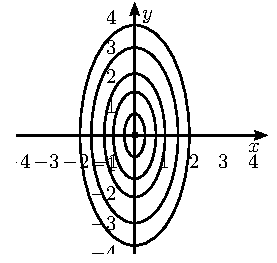
\includegraphics{figuras/fig18}
%     \label{fig18}
%   }
%   \quad
%   \subfloat[Gráfico: elips\'oide]{
%     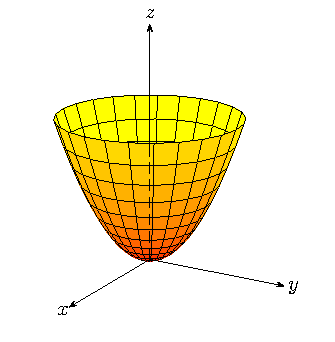
\includegraphics{figuras/fig19}
%     \label{fig19}
%   }
%   \caption{Elipse e elips\'oide}
% \end{figure}

% \end{sol}

% \begin{exem}
% Seja $f\left( {x,y} \right) = x^2 - y^2$

% Determine o domínio e a imagem, desenhe as curvas de nível e esboce o gráfico.
% \end{exem}

% \newpage 

% \begin{sol}
% \[
% \begin{gathered}
%   c < 0:f^{ - 1} \left( c \right) = \left\{ {\left( {x,y} \right) \in \R^2 :f\left( {x,y} \right) = c} \right\} \hfill \\
% \Rightarrow x^2  - y^2  = c < 0 \hfill \\
% \Rightarrow y^2  - x^2  =  - c > 0 \hfill \\
% c = 0:f\left( {x,y} \right) = 0 \hfill \\
% \Rightarrow x^2  - y^2  = 0 \hfill \\
% \Rightarrow x^2  = y^2  \hfill \\
% \Rightarrow \left| x \right| = \left| y \right| \hfill \\
% \Rightarrow y =  \pm x \hfill \\
% c > 0:x^2  - y^2  = c > 0 \hfill \\
% \end{gathered}
% \]

% Figuras (\ref{fig20}) e (\ref{fig21}).

% \begin{figure}[!h]
%   \centering
%   \subfloat[Curva de nível: hiperbol\'oide]{
%     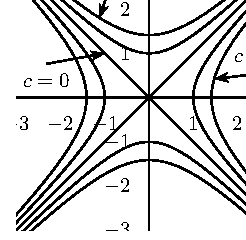
\includegraphics{figuras/fig20}
%     \label{fig20}
%   }
%   \quad
%   \subfloat[Gráfico: parabol\'oide hiperb\'olico]{
%     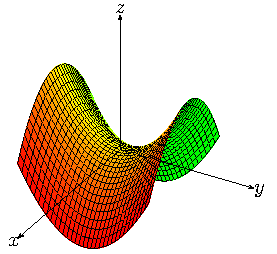
\includegraphics{figuras/fig21}
%     \label{fig21}
%   }
%   \caption{Hiperbol\'oide e parabol\'oide hiperb\'olico}
% \end{figure}

% \end{sol}

% \begin{exem}
% Seja $\displaystyle f\left( {x,y} \right) = \frac{y}{x - 1}$

% Determine o domínio e a imagem, desenhe as curvas de nível e esboce o gráfico.
% \end{exem}

% \newpage 

% \begin{sol}
% \[
% D_f  = \left\{ {x \in \R:x - 1 \ne 0} \right\}
% \]

% Fazendo

% \[
% \begin{gathered}
% \frac{y}
% {{x - 1}} = c \hfill \\
% y = c\left( {x - 1} \right) \hfill \\
% y = cx - c \hfill \\
% \end{gathered}
% \]

% % figura 22 Curva de nível: feixe de retas
% % figura 23 Gráfico

% % \begin{figure}[!h]
% %   \centering
% %   \subfloat[Curva de nível: feixe de retas]{
% %     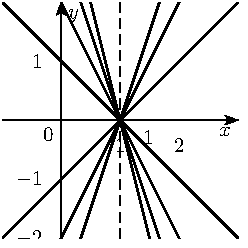
\includegraphics{figuras/fig22}
% %     \label{fig22}
% %   }
% %   \quad
% %   \subfloat[Gráfico]{
% %     \includegraphics{figuras/fig23}
% %     \label{fig23}
% %   }
% % \end{figure}

% \end{sol}

% \begin{exem}
% Seja $f\left( {x,y} \right) = \ln \left( {x - y} \right)$

% Determine o domínio e a imagem, desenhe as curvas de nível e esboce o gráfico.
% \end{exem}

% \begin{sol}
% \[
% D_f  = \left\{ {\left( {x,y} \right) \in \R^2 :x - y > 0} \right\}
% \]

% % figura 24 
% \myfig[height=3cm]{fig24}{Domínio de $f(x,y)$}

% \[
% \begin{gathered}
% \ln \left( {x - y} \right) = c \hfill \\
% \Rightarrow x - y = e^c  \hfill \\
% \Rightarrow y = x - e^c  \hfill \\
% \end{gathered}
% \]

% % figura 25 Curva de nível: feixe de retas paralelas
% % figura 26 Gráfico

% % % % % \begin{figure}[!h]
% % % % %   \centering
% % % % %   \subfloat[Curva de nível: feixe de retas paralelas]{
% % % % %     \includegraphics{figuras/fig25}
% % % % %     \label{fig25}
% % % % %   }
% % % % %   \quad
% % % % %   \subfloat[Gráfico]{
% % % % %     \includegraphics{figuras/fig26}
% % % % %     \label{fig26}
% % % % %   }
% % % % % \end{figure}

% \end{sol}

% \newpage

% \begin{exem}
% $f\left( {x,y,z} \right) = x^2  + y^2  + z^2$
% \end{exem}

% \begin{sol}
% \[
% \begin{gathered}
% c < 0:f^{ - 1} \left( c \right) = \emptyset  \hfill \\
%   c = 0:f^{ - 1} \left( 0 \right) = \left\{ {\left( {0,0,0} \right)} \right\} \hfill \\
% c > 0:x^2  + y^2  + z^2  = c > 0 \hfill \\
% \end{gathered}
% \]

% % \begin{figure}[!htb]
% %   \centering
% %   \includegraphics[width=3.5cm]{fig27}
% %   \caption{Curva de nível: conjunto de esferas.}\label{fig27a}
% % \end{figure}

% \myfig[width=3.5cm]{fig27bola}{Curva de nível: conjunto de esferas.}

% \textbf{Obs:} Impossível desenhar o gráfico de $f(x,y)$, pois está em $\R^4$.
% \end{sol}

% \begin{exem}
% $f\left( {x,y,z} \right) = x^2  + 4y^2  + z^2$
% \end{exem}

% \begin{sol}
% \[
% \begin{gathered}
% c < 0:f^{ - 1} \left( c \right) = \emptyset  \hfill \\
%   c = 0:f^{ - 1} \left( 0 \right) = \left\{ {\left( {0,0,0} \right)} \right\} \hfill \\
% c > 0:x^2  + 4y^2  + z^2  = c > 0 \hfill \\
% \end{gathered}
% \]

% % figura 28 Curva de nível: conjunto de elips\'oides

% % \myfig{fig28}{Curva de nível: conjunto de elips\'oides}
% \end{sol}

% \begin{exem}
% $f\left( {x,y,z} \right) = x^2  - y^2  - z^2$
% \end{exem}

% \section{Limite} \label{sec10}

% \begin{defi}[Ponto de acumulação]
% Seja $A \subset \R^n$ e $x_0 \in \R^n$. O ponto $x_0 \in \R^n$ é de \textit{acumulação}\index{Ponto!de acumulação} se $B_\varepsilon  \left( {x_0 } \right):\left\{ {x_0 } \right\} \cap A \ne \emptyset ,\forall \varepsilon  > 0$.
% \end{defi}

% \begin{exem}
% Seja $A = \left[ {0,1} \right]$.

% $1$ é ponto de acumulação.

% \tkzfig{fig30}{Limite}
% \end{exem}

% \begin{exem}
% Seja $A = \left[ {0,1} \right[ \cup \left\{ 2 \right\}$.

% $2$ não é ponto de acumulação.
% \end{exem}

% \begin{defi}[Limite]
%     Seja $f:A \subset \R^n  \to \R$ uma função e $x_0$ ponto de acumulação de $A$. Dizemos que $f$ tem \textit{limite}\index{Limite} $L$ em $x_0$ se dada uma bola centrada em $L$, $B_\varepsilon  \left( L \right)$, existe bola centrada em $x_0$, $B_\delta  \left( {x_0 } \right)$, tal que $f\left( {B_\delta  \left( {x_0 } \right) \cap A} \right) \subset B_\varepsilon  \left( L \right)$.

% \

% Notação: $\displaystyle \mathop {\lim }\limits_{x \to x_0 } f\left( x \right) = L$

% \

% Em outras palavras,

%     Dado $\varepsilon  > 0$, existe $\delta  > 0$ tal que $0 < \left\| {x - x_0 } \right\| < \delta  \Rightarrow \left| {f\left( x \right) - L} \right| < \varepsilon$.
% \end{defi}

% \begin{exem}
%     Seja $f:\R^2  - \left\{ {\left( {0,0} \right)} \right\} \to \R$ dado por $\displaystyle f\left( {x,y} \right) = \frac{{ - x^2  + y^2 }}{{x^2  + y^2 }}$. Calcule o limite da função quando $(x,y)$ tende a $(0,0)$.
% \end{exem}

% \begin{sol}
% Tomando duas retas que passam no ponto $(0,0)$, temos:

% $f\left( {x,0} \right) =  - 1$ e $f\left( {0,y} \right) = 1$

% Portanto, o limite não existe em $(0,0)$.
% \end{sol}

% \begin{teo}[Função Composta]\index{Função!composta}
%     Seja $A \subset \R^n$ e $x_0$ ponto de acumulação de $A$ $f:A \subset \R^n  \to \R$. Seja ainda $\gamma$ uma curva contínua tal que $\gamma \left( t \right) \in A,\forall t \ne t_0$ e $\gamma \left( {t_0 } \right) = x_0$.

%     Se $\mathop {\lim }\limits_{x \to x_0 } f\left( x \right) = L$, então $\mathop {\lim }\limits_{t \to t_0 } f\left( {\gamma \left( t \right)} \right) = L$.
% \end{teo}

% \begin{dem}
% Sejam

% \begin{eqnarray*}
% \gamma &:&\R \to \R^n  \hfill \\
% f&:&\R^n  \to \R \hfill \\
% f \circ \gamma &:&\R \to \R \hfill \\
% && t \to f\left( {\gamma \left( t \right)} \right) \hfill \\
% \end{eqnarray*}

%     Hip\'otese, $\mathop {\lim }\limits_{x \to x_0 } f\left( x \right) = L$, então, dada $B_\varepsilon  \left( L \right) \Rightarrow \exists B_\delta  \left( {x_0 } \right):f\left( {B_\delta  \left( {x_0 } \right) \cap A} \right) \subset B_\varepsilon  \left( L \right)$.

% % figura 32

%     $\gamma$ é contínua, então, dada $B_\delta  \underbrace {\left( {x_0 } \right)}_{\gamma \left( {t_0 } \right)}$, existe $B_r \left( {t_0 } \right)$ tal que $\gamma \left( {B_r \left( {t_0 } \right)} \right) \subset B_\delta  \left( {x_0 } \right)$

% \[
% \begin{gathered}
%   f\left( {\gamma \left( {B_r \left( {t_0 } \right)} \right)} \right) \subset f\left( {B_\delta  \left( {x_0 } \right) \cap A} \right) \subset B_\varepsilon  \left( L \right) \hfill \\
%    \Rightarrow \mathop {\lim }\limits_{t \to t_0 } f\left( {\gamma \left( t \right)} \right) = L \hfill \\
% \end{gathered}
% \]

% \end{dem}

% \textbf{Obs:} Se $\gamma_1$ e $\gamma_2$ são curvas como no teorema e $\mathop {\lim }\limits_{t \to t_0 } f\left( {\gamma _1 \left( t \right)} \right) \ne \mathop {\lim }\limits_{t \to t_0 } f\left( {\gamma _2 \left( t \right)} \right)$, então, $\nexists \mathop {\lim }\limits_{x \to x_0 } f\left( x \right)$.

% \begin{exem}
% No exemplo anterior usamos:
% \end{exem}

% \begin{sol}
%     $\gamma _1 \left( t \right) = \left( {t,0} \right)$ e $\gamma _2 \left( t \right) = \left( {0,t} \right)$,

%      então, $f\left( {\gamma _1 \left( t \right)} \right) = f\left( {t,0} \right) =  - 1$ e $f\left( {\gamma _2 \left( t \right)} \right) = f\left( {0,t} \right) = 1$
% \end{sol}

% \begin{teo}[do confronto]\index{Teorema!do confronto}
%     Sejam $A \subset \R^n$, $x_0$ ponto de acumulação de $A$ e $f,g,h$ funções de $A$ em $\R$ tais que $f\left( x \right) \leqslant g\left( x \right) \leqslant h\left( x \right)$ para $x \in B_r \left( {x_0 } \right) \cap A$

%     se $\mathop {\lim }\limits_{x \to x_0 } f\left( x \right) = \mathop {\lim }\limits_{x \to x_0 } h\left( x \right) = L$ então, $\mathop {\lim }\limits_{x \to x_0 } h\left( x \right) = L$.
% \end{teo}

% \begin{dem}
%     $\mathop {\lim }\limits_{x \to x_0 } f\left( x \right) = L \Rightarrow$ dada $B_\varepsilon  \left( L \right)$ existe $B_{\delta _1 } \left( {x_0 } \right)$ tal que $f\left( {B_{\delta _1 } \left( {x_0 } \right) \cap A} \right) \subset B_\varepsilon  \left( L \right)$

%     $\mathop {\lim }\limits_{x \to x_0 } h\left( x \right) = L \Rightarrow$ dada $B_\varepsilon  \left( L \right)$ existe $B_{\delta _2 } \left( {x_0 } \right)$ tal que $h\left( {B_{\delta _2 } \left( {x_0 } \right) \cap A} \right) \subset B_\varepsilon  \left( L \right)$

%     Seja $z \in B_{\delta _1 } \left( {x_0 } \right) \cap B_{\delta _2 } \left( {x_0 } \right) \cap A$, então

% \[
% \begin{gathered}
%       f\left( z \right) \leqslant g\left( z \right) \leqslant h\left( z \right) \hfill \\
%       \left| {f\left( z \right) - L} \right| < \varepsilon  \Rightarrow \underbrace { - \varepsilon  < f\left( z \right) - L}_{} < \varepsilon  \hfill \\
%       \left| {h\left( z \right) - L} \right| < \varepsilon  \Rightarrow  - \varepsilon  < \underbrace {h\left( z \right) - L < \varepsilon }_{} \hfill \\
%        - \varepsilon  < f\left( z \right) - L \leqslant g\left( x \right) - L \leqslant h\left( z \right) - L < \varepsilon  \hfill \\
% \left| {g\left( x \right) - L} \right| < \varepsilon  \hfill \\
%        \Rightarrow \mathop {\lim }\limits_{x \to x_0 } g\left( x \right) = L \hfill \\
% \end{gathered}
% \]

% \end{dem}

% \begin{cor}
%     Sejam $A \subset \R^n$, $x_0$ ponto de acumulação de $A$ e $f,g$ funções de $A$ em $\R$ com $\left| {g\left( x \right)} \right| < M$ (limitada), para $x \in B_r \left( {x_0 } \right) \cap A$ e $\mathop {\lim }\limits_{x \to x_0 } f\left( x \right) = 0$. Então, $\mathop {\lim }\limits_{x \to x_0 } f\left( x \right)g\left( x \right) = 0$.
% \end{cor}

% \begin{dem}
% \[
% \begin{gathered}
%   \left| {f\left( x \right)g\left( x \right)} \right| < \left| {f\left( x \right)} \right|M \hfill \\
%    - M\left| {f\left( x \right)} \right| < f\left( x \right)g\left( x \right) < M\left| {f\left( x \right)} \right| \hfill \\
%   \mathop {\lim }\limits_{x \to x_0 }  \pm M\left| {f\left( x \right)} \right| = 0 \hfill \\
%    \Rightarrow \mathop {\lim }\limits_{x \to x_0 } f\left( x \right)g\left( x \right) = 0 \hfill \\
% \end{gathered}
% \]

% \end{dem}

% \textbf{Exercícios}

% Prove que:

% \begin{exer}
%     $\mathop {\lim }\limits_{x \to x_0 } \left| {f\left( x \right)} \right| = 0 \Leftrightarrow \mathop {\lim }\limits_{x \to x_0 } f\left( x \right) = 0$
% \end{exer}

% \begin{exer}
%     $\mathop {\lim }\limits_{x \to x_0 } f\left( x \right) - L = 0 \Leftrightarrow \mathop {\lim }\limits_{x \to x_0 } f\left( x \right) = L$
% \end{exer}

% \begin{exer}
%     $\mathop {\lim }\limits_{x \to x_0 } f\left( x \right) = L \Leftrightarrow \mathop {\lim }\limits_{h \to 0} f\left( {x_0  + h} \right) = L,\left( {h \in \R^n } \right)$
% \end{exer}

% \begin{exer}
%     Se $\mathop {\lim }\limits_{x \to x_0 } f\left( x \right) > 0$, então, $\exists B_r \left( {x_0 } \right)$ tal que $f\left( x \right) > 0,\forall x \in B_r \left( {x_0 } \right)$.
% \end{exer}

% \textbf{Nota:} As propriedades de limite são as mesmas das funções de uma variável.

% \begin{exem}
%     Calcule $\mathop {\lim }\limits_{\left( {x,y} \right) \to \left( {0,0} \right)} \frac{{x^3 }}{{x^2  + y^2 }}$
% \end{exem}

% \begin{sol}
% \[
%     \mathop {\lim }\limits_{\left( {x,y} \right) \to \left( {0,0} \right)} \frac{{x^3 }}{{x^2  + y^2 }} = \mathop {\lim }\limits_{\left( {x,y} \right) \to \left( {0,0} \right)} x\overbrace {\frac{{x^2 }}
% {{x^2  + y^2 }}}^{{\text{limitada}}} = 0
% \]

%     Pois $0 \leqslant x^2  \leqslant x^2  + y^2  \Rightarrow 0 \leqslant \frac{{x^2 }}
% {{x^2  + y^2 }} \leqslant 1$ é limitada.
% \end{sol}

% \begin{exem}
%     Calcule $\mathop {\lim }\limits_{\left( {x,y} \right) \to \left( {0,0} \right)} \frac{{x^2 }}{{x^2  + y^2 }}$
% \end{exem}

% \begin{sol}
% Tomemos duas curvas:

% \[
% \begin{gathered}
%   \gamma _1 \left( t \right) = \left( {t,0} \right) \Rightarrow f\left( {\gamma _1 \left( t \right)} \right) = f\left( {t,0} \right) = \frac{{t^2 }}
% {{t^2  + 0}} = 1 \Rightarrow \mathop {\lim }\limits_{t \to 0} f\left( {\gamma _1 \left( t \right)} \right) = 1 \hfill \\
%   \gamma _2 \left( t \right) = \left( {0,t} \right) \Rightarrow f\left( {\gamma _2 \left( t \right)} \right) = f\left( {0,t} \right) = \frac{0}
% {{0 + t^2 }} = 0 \Rightarrow \mathop {\lim }\limits_{t \to 0} f\left( {\gamma _2 \left( t \right)} \right) = 0 \hfill \\
%   \therefore \mathop {\lim }\limits_{t \to 0} f\left( {\gamma _1 \left( t \right)} \right) \ne \mathop {\lim }\limits_{t \to 0} f\left( {\gamma _2 \left( t \right)} \right) \hfill \\
% \end{gathered}
% \]

% Portanto, o limite não existe em $(0,0)$.
% \end{sol}

% \begin{exem}
%     Calcule $\mathop {\lim }\limits_{\left( {x,y} \right) \to \left( {0,0} \right)} \frac{{x^4 \sin \left( {x^2  + y^2 } \right)}}{{x^4  + y^2 }}$
% \end{exem}

% \begin{sol}
% \[
% \mathop {\lim }\limits_{\left( {x,y} \right) \to \left( {0,0} \right)} \frac{{x^4 \sin \left( {x^2  + y^2 } \right)}}
% {{x^4  + y^2 }} = \mathop {\lim }\limits_{\left( {x,y} \right) \to \left( {0,0} \right)} \overbrace {\frac{{x^4 }}
% {{x^4  + y^2 }}}^{{\text{limitada}}}\sin \left( {x^2  + y^2 } \right) = 0
% \]

% \end{sol}

% \begin{exem}
%     Calcule $\mathop {\lim }\limits_{\left( {x,y} \right) \to \left( {0,0} \right)} \frac{{xy}}
% {{2x - y^7 }}$
% \end{exem}

% \begin{sol}
%     Se tomarmos $\gamma _1 \left( t \right) = \left( {t,0} \right)$ e $\gamma _2 \left( t \right) = \left( {0,t} \right)$

% \[
%      \Rightarrow \mathop {\lim }\limits_{t \to 0} f\left( {\gamma _1 \left( t \right)} \right) = \mathop {\lim }\limits_{t \to 0} f\left( {\gamma _2 \left( t \right)} \right) = 0
% \]

%     Mas não é suficiente, pois pode haver infinitas curvas que passem no ponto, então, vamos usar as curvas de nível para ver o comportamento da função.

% Curva de nível de $f: f(x,y)=c$

% \[
% \begin{gathered}
% \frac{{xy}}
% {{2x - y^7 }} = c \Rightarrow x = \frac{{y^7 c}}
% {{2c - y}} \hfill \\
% \gamma \left( t \right) = \left( {\frac{{t^7 c}}
% {{2c - t}},t} \right) \hfill \\
% t = 0 \Rightarrow \gamma \left( 0 \right) = \left( {0,0} \right) \hfill \\
%   f\left( {\gamma \left( t \right)} \right) = c \Rightarrow \mathop {\lim }\limits_{t \to 0} f\left( {\gamma \left( t \right)} \right) = c \hfill \\
% \end{gathered}
% \]

%     O limite de $f\left( {\gamma \left( t \right)} \right)$ pode assumir qualquer valor. Portanto, o limite de $f(x,y)$ não existe em $(0,0)$.
% \end{sol}

% \section{Continuidade} \label{sec11}

% \begin{defi}
%     Sejam $A \subset \R^n$, $x_0 \in A$ ponto de acumulação de $A$. Dizemos que $f$ é \textit{contínua}\index{Função!contínua} em $x_0$ se

% \[\boxed{
%     \mathop {\lim }\limits_{x \to x_0 } f\left( x \right) = f\left( {x_0 } \right)}
% \]

% \end{defi}

% \begin{exem}
% \begin{equation*}
% f(x,y)=\left\{ \begin{array}{cl}\displaystyle
%         \frac{{x^2  - y^2 }}{{x^2  + y^2 }} & \textrm{se }\left( {x,y} \right) \ne \left( {0,0} \right)\\
%         0 & \textrm{se }\left( {x,y} \right) = \left( {0,0} \right)\end{array}\right.
% \end{equation*}
% \end{exem}

% \begin{sol}
%     $\displaystyle \mathop {\lim }\limits_{\left( {x,y} \right) \to \left( {0,0} \right)} f\left( {x,y} \right) = \mathop {\lim }\limits_{\left( {x,y} \right) \to \left( {0,0} \right)} \frac{{x^2  - y^2 }}{{x^2  + y^2 }}$ não existe, pois, tomando $(t,0)$ e $(0,t)$ verificamos limites diferentes. Então $f$ não é contínua em $(0,0)$ mas nos outros pontos ela é.
% \end{sol}

% \begin{exem}
% \begin{equation*}
% f(x,y)=\left\{ \begin{array}{cl}\displaystyle
% \frac{{x^4 \sin \left( {x^2  + y^2 } \right)}}
%         {{x^4  + y^2 }} & \textrm{se }\left( {x,y} \right) \ne \left( {0,0} \right)\\
%         0 & \textrm{se }\left( {x,y} \right) = \left( {0,0} \right)\end{array}\right.
% \end{equation*}

% \end{exem}

% \begin{sol}
%     A função é contínua em $(0,0)$, $\mathop {\lim }\limits_{\left( {x,y} \right) \to \left( {0,0} \right)} f\left( {x,y} \right) = 0 = f\left( 0 \right)$.
% \end{sol}

% \begin{exem}
% \begin{equation*}
% f(x,y)=\left\{ \begin{array}{cl}\displaystyle
% \frac{{x^2 \sin \left( \displaystyle {\frac{{x^2 y^8 }}
%         {{y^8  + x^4 }}} \right)}}{{x^2  + y^2 }} & \textrm{se }\left( {x,y} \right) \ne \left( {0,0} \right)\\
%         0 & \textrm{se }\left( {x,y} \right) = \left( {0,0} \right)\end{array}\right.
% \end{equation*}

% \end{exem}

% \begin{sol}
%     $\displaystyle \frac{{x^2 }}{{x^2  + y^2 }}$ é limitada e $\displaystyle \sin \left( {\frac{{x^2 y^8 }}{{y^8  + x^4 }}} \right)$ também é limitada, mas não resolve a equação, mas $\displaystyle \frac{{y^8 }}{{y^8  + x^4 }}$ é limitada, então, $\mathop {\lim }\limits_{\left( {x,y} \right) \to \left( {0,0} \right)} \sin x^2  = 0$.

% \[
%     \mathop {\lim }\limits_{\left( {x,y} \right) \to \left( {0,0} \right)} f\left( {x,y} \right) = 0 \ne f\left( 0 \right) = 1
% \]

% Portanto, $f(x,y)$ não é contínua em $(0,0)$.

% \end{sol}

% \begin{teo}
%     Sejam $A \subset \R^n ,B \subset \R$ e funções $f:A \to \R$ e $g:B \to \R$ tal que $f\left( A \right) \subset B$. Se $f$ é contínua em $x_0$ e $g$ é contínua em $f\left( {x_0 } \right)$ então, $g \circ f$ é contínua em $x_0$.
% \end{teo}

% \begin{dem}
% $g$ é contínua em $f\left( {x_0 } \right)$
%     $\Rightarrow$ dado $B_\varepsilon  \left( {g\left( {f\left( {x_0 } \right)} \right)} \right)$ existe $B_{\delta _1 } \left( {f\left( {x_0 } \right)} \right)$ tal que

% \[
%     g\left( {B_{\delta _1 } \left( {f\left( {x_0 } \right)} \right) \cap A} \right) \subset B_\varepsilon  \left( {g\left( {f\left( {x_0 } \right)} \right)} \right)
% \]

%     $f$ é contínua em $x_0$ $\Rightarrow \mathop {\lim }\limits_{x \to x_0 } f\left( x \right) = f\left( {x_0 } \right)$

%     $\Rightarrow$ para $B_{\delta _1 } \left( {f\left( {x_0 } \right)} \right)$ existe $B_{\delta _2 } \left( {x_0 } \right)$ tal que

% \[
%     f\left( {B_{\delta _2 } \left( {x_0 } \right) \cap A} \right) \subset B_{\delta _1 } \left( {f\left( {x_0 } \right)} \right)
% \]

% \[
%     g\left( {f\left( {B_{\delta _2 } \left( {x_0 } \right) \cap A} \right)} \right) \subset g\left( {B_{\delta _1 } \left( {f\left( {x_0 } \right)} \right)} \right) \subset B_\varepsilon  \left( {g\left( {f\left( {x_0 } \right)} \right)} \right)
% \]

%     $\Rightarrow \mathop {\lim }\limits_{x \to x_0 } \left( {g \circ f} \right)\left( x \right) = g\left( {f\left( {x_0 } \right)} \right) \Rightarrow g \circ f$ é contínua em $x_0$.
% \end{dem}

% \begin{teo}
%     Sejam $A \subset \R^n ,I \subset \R,f:A \to \R,\gamma :I \to \R^n ,\gamma \left( I \right) \subset A$. Se $\gamma$ é contínua em $t_0 \in I$ e $f$ é contínua em $\gamma \left( {t_0 } \right) \in A$ então, $f \circ \gamma$ é contínua em $t_0$.

% \end{teo}

% \chapter{Derivadas} \label{chap03}

% \section{Derivadas Parciais} \label{sec12}

% \begin{defi}
%     Seja $A \subset \R^n$ e $x_0$ ponto interior de $A$. Definimos a \textit{derivada parcial}\index{Derivada!parcial} de $f$ em $x_0$ na direção $e_i$ (base can\^onica) por

% \[\boxed{
%     \frac{{\partial f}}{{\partial x_i }}\left( {x_0 } \right) = \mathop {\lim }\limits_{h \to 0} \frac{{f\left( {x_0  + he_i } \right) - f\left( {x_0 } \right)}}{h}}
% \]

% \end{defi}

% Na prática, basta derivar $f$ em relação \`a varíável $x_i$, considerando as outras como constantes.

% \begin{exem}
% $f\left( {x,y} \right) = \arctan \left( {x^2  + y^2 } \right)$
% \end{exem}

% \begin{sol}
% \[
% \begin{gathered}
% \frac{{\partial f}}
% {{\partial x}}\left( {x,y} \right) = \frac{1}
% {{1 + \left( {x^2  + y^2 } \right)}}2x \hfill \\
% \frac{{\partial f}}
% {{\partial y}}\left( {x,y} \right) = \frac{1}
% {{1 + \left( {x^2  + y^2 } \right)}}2y \hfill \\
% \end{gathered}
% \]
% \end{sol}

% \begin{exem}
% $z = f\left( {x,y} \right)$ é solução da equação $x^2  + y^2  + z^2  = 1$.
% \end{exem}

% \begin{sol}
% Note que $z^2 \left( {x,y} \right)$. Derivando em $x$, temos:

% \[
% \begin{gathered}
% 2x + 2z\frac{{\partial f}}{{\partial x}} = 0 \hfill \\
%       \frac{{\partial f}}{{\partial x}} =  - \frac{x}{{f\left( {x,y} \right)}} \hfill \\
% \frac{{\partial f}}{{\partial y}} =  - \frac{y}
% {{f\left( {x,y} \right)}} \hfill \\
% \end{gathered}
% \]

% \end{sol}

% \begin{exem}
%     Suponha $f$ contínua e $\frac{{\partial f}}{{\partial x}}$ existe. Então, $\frac{{\partial f}}{{\partial x}} = 0$.
% \end{exem}

% \begin{sol}
% $f$ não varia na direção do eixo $x$.
% \end{sol}

% \begin{exem}
% Seja
% \begin{equation*}
% f(x,y)=\left\{ \begin{array}{cl}\displaystyle
%         \frac{{x^3  - y^2 }}{{x^2  + y^2 }} & \textrm{se }\left( {x,y} \right) \ne \left( {0,0} \right)\\
%         0 & \textrm{se }\left( {x,y} \right) = \left( {0,0} \right)\end{array}\right.
% \end{equation*}
% \end{exem}

% \begin{sol}
%     Nos pontos $\left( {x,y} \right) \ne \left( {0,0} \right)$ podemos aplicar a regra do quociente

% \[
% \begin{gathered}
% \frac{{\partial f}}
% {{\partial x}}\left( {x,y} \right) = \frac{{3x^2 \left( {x^2  + y^2 } \right) - \left( {x^3  - y^2 } \right)2x}}
% {{\left( {x^2  + y^2 } \right)^2 }} \hfill \\
% \frac{{\partial f}}
% {{\partial x}}\left( {x,y} \right) = \frac{{x^4  + 3x^2 y^2  + 2xy^2 }}
% {{\left( {x^2  + y^2 } \right)^2 }} \hfill \\
% \frac{{\partial f}}
% {{\partial y}}\left( {x,y} \right) =  - \frac{{2x^2 y\left( {1 + x} \right)}}
% {{\left( {x^2  + y^2 } \right)^2 }} \hfill \\
% \end{gathered}
% \]

% Em $(0,0)$, temos:

% \begin{eqnarray*}
%   \frac{{\partial f}}{{\partial x}}\left( {0,0} \right) &=& \mathop {\lim }\limits_{h \to 0} \frac{{f\left( {\left( {0,0} \right) + h\left( {1,0} \right)} \right) - f\left( {0,0} \right)}}{h} \hfill \\
%    &=& \mathop {\lim }\limits_{h \to 0} \frac{{f\left( {h,0} \right) - f\left( {0,0} \right)}}{h} \hfill \\
% &=& \mathop {\lim }\limits_{h \to 0} \frac{{h - 0}}
% {h} = 1 \hfill \\
%   \frac{{\partial f}}{{\partial y}}\left( {0,0} \right) &=& \mathop {\lim }\limits_{h \to 0} \frac{{f\left( {0,h} \right) - f\left( {0,0} \right)}}{h} \hfill \\
% &=& \mathop {\lim }\limits_{h \to 0} \frac{{ - 1 - 0}}{h} \hfill \\
% \end{eqnarray*}

% que não existe.
% \end{sol}

% \textbf{Interpretação geométrica das derivadas parciais}

% % figura 33

% \section{Derivadas Direcionais} \label{sec13}

% \begin{defi}
%     Seja $f:A \subset \R^n \to \R$ e $x_0$ ponto interior de $A$ e $v$ um vetor unitário de $\R^n$. Definimos a \textit{derivada direcional}\index{Derivada!direcional} de $f$ em $x_0$ na direção de $v$ por

% \[\boxed{
%     \frac{{\partial f}}{{\partial v }}\left( {x_0 } \right) = \mathop {\lim }\limits_{h \to 0} \frac{{f\left( {x_0  + hv } \right) - f\left( {x_0 } \right)}}{h}}
% \]

% \end{defi}

% \begin{exem}
% Seja
% \begin{equation*}
% f(x,y)=\left\{ \begin{array}{cl}\displaystyle
%         \frac{{xy^3}}{{x^2  + y^6 }} & \textrm{se }\left( {x,y} \right) \ne \left( {0,0} \right)\\
%         0 & \textrm{se }\left( {x,y} \right) = \left( {0,0} \right)\end{array}\right.
% \end{equation*}

% Calcule $\frac{{\partial f}}{{\partial v}}\left( {0,0} \right)$.
% \end{exem}

% \begin{sol}
% Seja $v = \left( {a,b} \right) \in \R^2$ com $a^2 + b^2 = 1$.

% \begin{eqnarray*}\displaystyle
%   \frac{{\partial f}}{{\partial v}}\left( {0,0} \right) &=& \mathop {\lim }\limits_{h \to 0} \frac{{f\overbrace {\left( {\left( {0,0} \right) + h\left( {a,b} \right)} \right)}^{\left( {ha,hb} \right)} - f\left( {0,0} \right)}}{h} \hfill \\
%    &=& \mathop {\lim }\limits_{h \to 0} \frac{{\displaystyle  \frac{{h^4 ab^3 }}{{h^2 \left( {a^2  + h^4 b^6 } \right)}} - 0}}
% {h} = 0 \hfill \\
% \end{eqnarray*}

% Então, existe a derivada direcional e é igual a $0$ em todas as direções.

% Vamos ver agora se $f$ é contínua.

% Seja $\gamma \left( t \right) = \left( {t^3 ,t} \right)$

% \[
%     \mathop {\lim }\limits_{t \to 0} f\left( {\gamma \left( t \right)} \right) = \mathop {\lim }\limits_{t \to 0} \frac{{t^6 }}{{t^6  + t^6 }} = \frac{1}{2}\left( { \ne 0 = f\left( {0,0} \right)} \right)
% \]

% Portanto, $f$ não é contínua em $(0,0)$.
% \end{sol}

% \section{Diferenciabilidade de Funções de $\R^n$ a valores reais} \label{sec14}

% Relembrando Cálculo I, temos:

% $f$ é derivável em $x_0$ se

% \[
% \begin{gathered}
%   \mathop {\lim }\limits_{h \to 0} \frac{{f\left( {x_0  + h} \right) - f\left( {x_0 } \right)}}
% {h} = f'\left( {x_0 } \right) \hfill \\
%    \Rightarrow \mathop {\lim }\limits_{h \to 0} \frac{{f\left( {x_0  + h} \right) - f\left( {x_0 } \right) - hf'\left( {x_0 } \right)}}
% {h} = 0 \hfill \\
%    \Leftrightarrow \mathop {\lim }\limits_{h \to 0} \frac{{f\left( {x_0  + h} \right) - f\left( {x_0 } \right) - f'\left( {x_0 } \right)h}}
% {{\left| h \right|}} = 0 \hfill \\
% \end{gathered}
% \]

% Onde $f'\left( {x_0 } \right)$ é um n\'umero real que deve existir e $h$ é um vetor.

% \begin{defi}[Transformação linear]
% \begin{sloppypar}
% Uma \textit{transformação linear}\index{Transformação!linear} ${T:\R^n  \to \R^m}$ é uma função tal que
% \end{sloppypar}


% \begin{enumerate}[i)]
%       \item $T\left( {x + y} \right) = T\left( x \right) + T\left( y \right),\forall x,y \in \R^n$
%       \item $T\left( {\alpha x} \right) = \alpha T\left( x \right),\forall x \in \R^n {\text{ e }}\forall \alpha  \in \R$
% \end{enumerate}
% \end{defi}

% \begin{defi}
%     A matriz de $T$ nas bases can\^onicas de $\R^n$ e $\R^m$ é $\left[ T \right] = \left( {a_{ij} } \right)_{m \times n}$ onde $a_{ij}  = T\left( {e_j } \right)_i$ (i-ésima coordenada de $T\left( {e_j } \right)$, $e_j$ da base can\^onica de $\R^n$).

%     Usando isso, temos, $T\left( x \right) = \left[ T \right]_{m \times n} X_{n + 1}$.

%     Quando $n=1$, $f$ ser diferenciável em $x_0$ é dizer que existe $T_{x_0 } :\R \to \R$ tal que

% \[
%     \mathop {\lim }\limits_{h \to 0} \frac{{f\left( {x_0  + h} \right) - f\left( {x_0 } \right) - T_{x_0 } \left( h \right)}}{{\left| h \right|}} = 0
% \]

% e nesse caso, $\left[ T \right] = f'\left( {x_0 } \right)$.
% \end{defi}

% \begin{defi}[Função diferenciável]
%     Seja $A \subset \R^n$, $x_0$ ponto interior de $A$ e $f:A \to \R$. Dizemos que $f$ é diferenciável em $x_0$ se existir $T_{x_0 } :\R^n  \to \R$ linear tal que

% \[\boxed{
%     \mathop {\lim }\limits_{h \to 0} \frac{{f\left( {x_0  + h} \right) - f\left( {x_0 } \right) - T_{x_0 } \left( h \right)}}{{\left\| h \right\|}} = 0} \left( 1 \right)
% \]

%     Onde: $\left\| h \right\|$ é a norma do vetor devido ao $\R^n$ e $h \in \R^n$.
% \end{defi}

% \newpage 

% \begin{teo}
% Se existe ${T_{x_0 } }$ nas condições acima então ela é \'unica.
% \end{teo}

% \begin{dem}
%     Sejam ${T_{x_0 } }$ e ${L_{x_0 } }$ transformações lineares de $\R^n$ em $\R$ satisfazendo a equação $(1)$, então

% \[
%     \mathop {\lim }\limits_{h \to 0} \frac{{f\left( {x_0  + h} \right) - f\left( {x_0 } \right) - T_{x_0 } \left( h \right)}}{{\left\| h \right\|}} = 0
% \]

% e

% \[
% \begin{gathered}
%       \mathop {\lim }\limits_{h \to 0} \frac{{f\left( {x_0  + h} \right) - f\left( {x_0 } \right) - L_{x_0 } \left( h \right)}}{{\left\| h \right\|}} = 0 \hfill \\
%        \Rightarrow \mathop {\lim }\limits_{h \to 0} \frac{{T_{x_0 } \left( h \right) - L_{x_0 } \left( h \right)}}{{\left\| h \right\|}} = 0 \hfill \\
% \end{gathered}
% \]

% Escolha $h = h_i e_i$, $e_i$ é da base can\^onica de $\R^n$.

% \[
% \begin{gathered}
%       \mathop {\lim }\limits_{h \to 0} \frac{{T_{x_0 } \left( {h_i e_i } \right) - L_{x_0 } \left( {h_i e_i } \right)}}{{\left\| {h_i e_i } \right\|}} = 0 \hfill \\
%        \Rightarrow \mathop {\lim }\limits_{h \to 0} \frac{{h_i \left( {T_{x_0 } \left( {e_i } \right) - L_{x_0 } \left( {e_i } \right)} \right)}}{{\left| {h_i } \right|}} = 0 \hfill \\
% \end{gathered}
% \]

%     Como, $\mathop {\lim }\limits_{h_i  \to 0} \frac{{h_i }}{{\left| {h_i } \right|}} = \nexists$ não existe

% \[
% \begin{gathered}
%    \Rightarrow T_{x_0 } \left( {e_i } \right) - L_{x_0 } \left( {e_i } \right) = 0 \hfill \\
%    \Rightarrow T_{x_0 } \left( {e_i } \right) = L_{x_0 } \left( {e_i } \right),\forall i = 1,2,...,n \hfill \\
% \Rightarrow L_{x_0 }  = T_{x_0 }  \hfill \\
% \end{gathered}
% \]

% \end{dem}

% \begin{teo}
%     Seja $A \subset \R^n$, $f:A \to \R$, diferenciável em $x_0$, então

% \[
% \left[ {T_{x_0 } } \right] = \left[ {\begin{array}{*{20}c}\displaystyle
%     {\frac{{\partial f}}{{\partial x_1 }}\left( {x_0 } \right)} & \displaystyle {\frac{{\partial f}}{{\partial x_2 }}\left( {x_0 } \right)} &  \cdots  & \displaystyle {\frac{{\partial f}}{{\partial x_n }}\left( {x_0 } \right)}  \\
% \end{array} } \right]_{1 \times n}
% \]

% \end{teo}

% \begin{dem}
% $f$ é diferenciável em $x_0$, então

% \[
%     \mathop {\lim }\limits_{h \to 0} \frac{{f\left( {x_0  + h} \right) - f\left( {x_0 } \right) - T_{x_0 } \left( h \right)}}{{\left\| h \right\|}} = 0
% \]

% Com $h = h_i e_i$, com $h_i \to 0$, temos

% \[
% \begin{gathered}
%   \mathop {\lim }\limits_{h_i  \to 0} \frac{{f\left( {x_0  + h_i e_i } \right) - f\left( {x_0 } \right) - h_i T_{x_0 } \left( {e_i } \right)}}
% {{h_i }} = 0 \hfill \\
%    \Rightarrow \mathop {\lim }\limits_{h_i  \to 0} \frac{{f\left( {x_0  + h_i e_i } \right) - f\left( {x_0 } \right)}}
% {{h_i }} - \mathop {\lim }\limits_{h_i  \to 0} \frac{{\bcancel{h_i} T_{x_0 } \left( {e_i } \right)}}{{\bcancel{h_i} }} = 0 \hfill \\
% \Rightarrow \frac{{\partial f}}
% {{\partial x_i }}\left( {x_0 } \right) - T_{x_0 } \left( {e_i } \right) = 0 \hfill \\
% \Rightarrow T_{x_0 } \left( {e_i } \right) = \frac{{\partial f}}
% {{\partial x_i }}\left( {x_0 } \right),i = 1,2,...,n \hfill \\
% \end{gathered}
% \]

% \end{dem}

% \textbf{Nota:} $T_{x_0 }$ é a diferencial de $f$ em $x_0$.

% \begin{teo}
%     Seja $f:A \subset \R^n \to \R$ diferenciável em $x_0$. Então, $f$ é contínua em $x_0$.
% \end{teo}

% \begin{dem}
%     Seja $E\left( h \right) = f\left( {x_0  + h} \right) - f\left( {x_0 } \right) - T_{x_0} \left( h \right)$, $f$ é diferenciável em $x_0$, então

% \[
%     \mathop {\lim }\limits_{h \to 0} \frac{{E\left( h \right)}}{{\left\| h \right\|}} = 0
% \]

% $T_{x_0}$ é contínua

% \[
% \begin{gathered}
%    \Rightarrow \mathop {\lim }\limits_{h \to 0} T_{x_0 } \left( h \right) = T\left( 0 \right) = 0 \hfill \\
%   \mathop {\lim }\limits_{h \to 0} E\left( h \right) = \mathop {\lim }\limits_{h \to 0} \overbrace {\left\| h \right\|}^0\overbrace {\frac{{E\left( h \right)}}
% {{\left\| h \right\|}}}^0 = 0 \hfill \\
%   0 = \mathop {\lim }\limits_{h \to 0} E\left( h \right) = \mathop {\lim }\limits_{h \to 0} \left( {f\left( {x_0  + h} \right) - f\left( {x_0 } \right) - T_{x_0 } \left( h \right)} \right) \hfill \\
%   0 = \mathop {\lim }\limits_{h \to 0} \left( {f\left( {x_0  + h} \right) - f\left( {x_0 } \right)} \right) - \mathop {\lim }\limits_{h \to 0} \overbrace {T_{x_0 } \left( h \right)}^0 \hfill \\
%   \mathop {\lim }\limits_{h \to 0} f\left( {x_0  + h} \right) = f\left( {x_0 } \right) \hfill \\
% \end{gathered}
% \]

% Portanto, $f$ é contínua em $x_0$.
% \end{dem}

% \begin{exem}
% Seja
% \begin{equation*}
% f(x,y)=\left\{ \begin{array}{cl}\displaystyle
%         \frac{{x^3}}{{x^2 + y^2 }} & \textrm{se }\left( {x,y} \right) \ne \left( {0,0} \right)\\
%         0 & \textrm{se }\left( {x,y} \right) = \left( {0,0} \right)\end{array}\right.
% \end{equation*}

% Esta função é diferenciável em $(0,0)$?
% \end{exem}

% \begin{sol}
%     $f$ é contínua em $(0,0)$ (tem chance de ser diferenciável, mas o teorema diz o contrário.)

% Então, $f$ ser diferenciável em $(0,0)$

% $\Rightarrow \exists T_{x_0 } :\R^2  \to \R$ tal que

% \[
%     \mathop {\lim }\limits_{h \to 0} \frac{{f\left( {x_0  + h} \right) - f\left( {x_0 } \right) - T_{x_0 } \left( h \right)}}{{\left\| h \right\|}} = 0
% \]

% Melhorando, para $\R^2  \to \R$ temos

% \[
%     \mathop {\lim }\limits_{\left( {h,k} \right) \to \left( {0,0} \right)} \frac{{f\left( {\left( {0,0} \right) + \left( {h,k} \right)} \right) - f\left( {0,0} \right) - T_{\left( {0,0} \right)} \left( {h,k} \right)}}{{\left\| {\left( {h,k} \right)} \right\|}} = 0
% \]

% Se existe $T_{\left( {0,0} \right)}$, ela é \'unica e

% \[
% \left[ {T_{\left( {0,0} \right)} } \right] = \left[ {\begin{array}{*{20}c}
%     {\frac{{\partial f}}{{\partial x}}\left( {0,0} \right)} & {\frac{{\partial f}}{{\partial y}}\left( {0,0} \right)}  \\
% \end{array} } \right]
% \]

% Então,

% \[
% \begin{gathered}
% \frac{{\partial f}}
% {{\partial x}}\left( {0,0} \right) = \mathop {\lim }\limits_{h \to 0} \frac{{\overbrace {f\left( {h,0} \right)}^h - f\left( {0,0} \right)}}
% {h} = 1 \hfill \\
% \frac{{\partial f}}
% {{\partial y}}\left( {0,0} \right) = \mathop {\lim }\limits_{h \to 0} \frac{{\overbrace {f\left( {0,h} \right)}^0 - f\left( {0,0} \right)}}
% {h} = 0 \hfill \\
%    \Rightarrow T_{\left( {0,0} \right)} \left( {h,k} \right) = \left[ {T_{\left( {0,0} \right)} } \right]\left[ {\begin{array}{*{20}c}
% h  \\
% k  \\

% \end{array} } \right] = \left[ {\begin{array}{*{20}c}
% 1 & 0  \\

% \end{array} } \right]\left[ {\begin{array}{*{20}c}
% h  \\
% k  \\

% \end{array} } \right] = h \hfill \\
% \end{gathered}
% \]

% \[
% \begin{gathered}
%   \mathop {\lim }\limits_{\left( {h,k} \right) \to \left( {0,0} \right)} \frac{{f\left( {h,k} \right) - f\left( {0,0} \right) - h}}
% {{\sqrt {h^2  + k^2 } }} =  \hfill \\
%   \mathop {\lim }\limits_{\left( {h,k} \right) \to \left( {0,0} \right)} \frac{{\frac{{h^3 }}
% {{h^2  + k^2 }} - 0 - h}}
% {{\sqrt {h^2  + k^2 } }} = \mathop {\lim }\limits_{\left( {h,k} \right) \to \left( {0,0} \right)} \frac{{h^3  - h\left( {h^2  + k^2 } \right)}}
% {{\left( {h^2  + k^2 } \right)^{{\raise0.5ex\hbox{$\scriptstyle 3$}
% \kern-0.1em/\kern-0.15em
% \lower0.25ex\hbox{$\scriptstyle 2$}}} }} = \mathop {\lim }\limits_{\left( {h,k} \right) \to \left( {0,0} \right)} \frac{{ - hk^2 }}
% {{\left( {h^2  + k^2 } \right)^{{\raise0.5ex\hbox{$\scriptstyle 3$}
% \kern-0.1em/\kern-0.15em
% \lower0.25ex\hbox{$\scriptstyle 2$}}} }} \hfill \\
% \end{gathered}
% \]

% Vamos chamar $\displaystyle \frac{{ - hk^2 }}
% {{\left( {h^2  + k^2 } \right)^{{\raise0.5ex\hbox{$\scriptstyle 3$}
% \kern-0.1em/\kern-0.15em
% \lower0.25ex\hbox{$\scriptstyle 2$}}} }} = g\left( {h,k} \right)$

% Escolhendo $\gamma \left( t \right) = \left( {t,t} \right)$, temos:

% \[
% \mathop {\lim }\limits_{t \to 0} g\left( {\gamma \left( t \right)} \right) = \mathop {\lim }\limits_{t \to 0} \frac{{ - t^3 }}
% {{\left( {2t^2 } \right)^{{\raise0.5ex\hbox{$\scriptstyle 3$}
% \kern-0.1em/\kern-0.15em
% \lower0.25ex\hbox{$\scriptstyle 2$}}} }} = \mathop {\lim }\limits_{t \to 0} \frac{{ - 1}}
% {{2\sqrt 2 }}\frac{{t^3 }}
% {{\left| t \right|^3 }} = \nexists
% \]

% Logo, $f$ não é diferenciável em $(0,0)$.
% \end{sol}

% \begin{teo}
%     Seja $A \subset \R^n$, $x_0$ interior a $A$ e $f:A \to \R$. Se $\frac{{\partial f}}{{\partial x_i }}$ são contínuas em $x_0$, então $f$ é diferenciável em $x_0$.
% \end{teo}

% \begin{dem}
%     Como $A$ é aberto, existe uma bola aberta $B$ de centro $\left( {x_0 ,y_0 } \right)$, contida em $A$. Sejam $h$ e $k$ tais que $\left( {x_0  + h,y_0  + k} \right) \in B$. Temos

% \[
% \scriptstyle{f\left( {x_0  + h,y_0  + k} \right) - f\left( {x_0 ,y_0 } \right) = \underbrace {f\left( {x_0  + h,y_0  + k} \right) - f\left( {x_0 ,y_0  + k} \right)}_{\left( I \right)} + \underbrace {f\left( {x_0 ,y_0  + k} \right) - f\left( {x_0 ,y_0 } \right)}_{\left( {II} \right)}}
% \]

%     Fazendo $G\left( x \right) = f\left( {x,y_0  + k} \right)$, pelo TVM \ref{tvm} existe $\overline x$, entre $x_0$ e $x_0 + h$ tal que

% \[
% \left( I \right) = G\left( {x_0  + h} \right) - G\left( {x_0 } \right) = G'\left( {\overline x } \right)h = \frac{{\partial f}}
% {{\partial x}}\left( {\overline x ,y_0  + k} \right)h
% \]

% Do mesmo modo, existe $\overline y$, entre $y_0$ e $y_0 + k$ tal que

% \[
%     \left( {II} \right) = \frac{{\partial f}}{{\partial y}}\left( {x_0 ,\overline y } \right)k
% \]

% Assim,

% \[
% f\left( {x_0  + h,y_0  + k} \right) - f\left( {x_0 ,y_0 } \right) = \frac{{\partial f}}
% {{\partial x}}\left( {\overline x ,y_0  + k} \right)h + \frac{{\partial f}}
% {{\partial y}}\left( {x_0 ,\overline y } \right)k
% \]

%     Subtraindo a ambos os membros da igualdade acima $\frac{{\partial f}}{{\partial x}}\left( {x_0 ,y_0 } \right)h + \frac{{\partial f}}{{\partial y}}\left( {x_0 ,y_0 } \right)k$ obtemos:

% \[
% \begin{gathered}
%   f\left( {x_0  + h,y_0  + k} \right) - f\left( {x_0 ,y_0 } \right) - \frac{{\partial f}}
% {{\partial x}}\left( {x_0 ,y_0 } \right)h - \frac{{\partial f}}
% {{\partial y}}\left( {x_0 ,y_0 } \right)k =  \hfill \\
% = \left[ {\frac{{\partial f}}
% {{\partial x}}\left( {\overline x ,y_0  + k} \right) - \frac{{\partial f}}
% {{\partial x}}\left( {x_0 ,y_0 } \right)} \right]h + \left[ {\frac{{\partial f}}
% {{\partial y}}\left( {x_0 ,\overline y } \right) - \frac{{\partial f}}
% {{\partial y}}\left( {x_0 ,y_0 } \right)} \right]k \hfill \\
% \end{gathered}
% \]

% Segue que

% \[
% \begin{gathered}
%   \left| {\frac{{f\left( {x_0  + h,y_0  + k} \right) - f\left( {x_0 ,y_0 } \right) - \frac{{\partial f}}
% {{\partial x}}\left( {x_0 ,y_0 } \right)h - \frac{{\partial f}}
% {{\partial y}}\left( {x_0 ,y_0 } \right)k}}
% {{\left\| {\left( {h,k} \right)} \right\|}}} \right| \leqslant  \hfill \\
% \underbrace { \leqslant \left| {\frac{{\partial f}}
% {{\partial x}}\left( {\overline x ,y_0  + k} \right) - \frac{{\partial f}}
% {{\partial x}}\left( {x_0 ,y_0 } \right)} \right|}_{\left( {III} \right)}\overbrace {\frac{{\left| h \right|}}
% {{\sqrt {h^2  + k^2 } }}}^{{\text{limitada}}} +  \hfill \\
% + \underbrace {\left| {\frac{{\partial f}}
% {{\partial y}}\left( {x_0 ,\overline y } \right) - \frac{{\partial f}}
% {{\partial y}}\left( {x_0 ,y_0 } \right)} \right|}_{\left( {IV} \right)}\frac{{\left| h \right|}}
% {{\sqrt {h^2  + k^2 } }} \hfill \\
% \end{gathered}
% \]

%     Pela continuidade de $\frac{{\partial f}}{{\partial x}}$ e $\frac{{\partial f}}{{\partial y}}$ em $\left( {x_0 ,y_0 } \right)$, as expressões $(III)$ e $(IV)$ tendem a zero, quando $\left( {h,k} \right) \to \left( {0,0} \right)$, e, portanto,

% \[
% \mathop {\lim }\limits_{\left( {h,k} \right) \to \left( {0,0} \right)} \frac{{f\left( {x_0  + h,y_0  + k} \right) - f\left( {x_0 ,y_0 } \right) - \frac{{\partial f}}
% {{\partial x}}\left( {x_0 ,y_0 } \right)h - \frac{{\partial f}}
% {{\partial y}}\left( {x_0 ,y_0 } \right)k}}
% {{\left\| {\left( {h,k} \right)} \right\|}} = 0
% \]

% logo, $f$ é diferenciável em $\left( {x_0 ,y_0 } \right)$.

% \end{dem}

% \section{Espaço Tangente} \label{sec15}

% \begin{defi}
% Seja $f:A \subset \R^n \to \R$ diferenciável em $x_0$:

% \[
% \begin{gathered}
%   \mathop {\lim }\limits_{h \to 0} \frac{{f\left( {x_0  + h} \right) - f\left( {x_0 } \right) - T_{x_0 } \left( h \right)}}
% {{\left\| h \right\|}} = 0 \hfill \\
%    \Rightarrow \mathop {\lim }\limits_{x \to x_0 } \frac{{f\left( x \right) - f\left( {x_0 } \right) - T_{x_0 } \left( {x - x_0 } \right)}}
% {{\left\| {x - x_0 } \right\|}} = 0 \hfill \\
%    \Rightarrow \mathop {\lim }\limits_{x \to x_0 } \frac{{f\left( x \right) - f\left( {x_0 } \right) - \sum\limits_{i = 1}^n {\frac{{\partial f}}
% {{\partial x_i }}\left( {x_0 } \right)\left( {x_i  - x_{0_i } } \right)} }}
% {{\left\| {x - x_0 } \right\|}} = 0 \hfill \\
% \end{gathered}
% \]

% \textbf{Nota:} Pode-se escrever, $\frac{{\partial f}}{{\partial x}} = f_x$.

%     Então, seja, $T\left( x \right) = f\left( {x_0 } \right) + \sum\limits_{i = 1}^n {f_{x_i } \left( {x_0 } \right)\left( {x_i  - x_{0_i } } \right)}$

% Temos,  $E\left( x \right) = f\left( x \right) - T\left( x \right)$

%     Portanto, $\displaystyle \mathop {\lim }\limits_{x \to x_0 } \frac{{E\left( x \right)}}{{\left\| {x - x_0 } \right\|}} = 0$

%     Então, $T:A \to \R$ é a "melhor" aproximação afim de $f$ em torno de $x_0$.
% \end{defi}

% \begin{defi}
%     Seja $A \subset \R^n$ e $f:A \to \R$ diferenciável em $x_0$. O subespaço afim de $\R^{n + 1}$ dado por

% \[
% \begin{gathered}
%   x_{n + 1}  - f\left( {x_0 } \right) = \sum\limits_{i = 1}^n {f_{x_i } \left( {x_0 } \right)\left( {x_i  - x_{0_i } } \right)}  \hfill \\
% \boxed{x_{n + 1}  - f\left( {x_0 } \right) = \frac{{\partial f}}
% {{\partial x_1 }}\left( {x_0 } \right)\left( {x_1  - x_{0_1 } } \right) + ... + \frac{{\partial f}}
% {{\partial x_n }}\left( {x_0 } \right)\left( {x_n  - x_{0_n } } \right) \hfill }\\
% \end{gathered}
% \]

%     é chamado \textit{espaço tangente} ao gráfico de $f$ em $\left( {x_0 ,f\left( {x_0 } \right)} \right),T_{\left( {x_0 ,f\left( {x_0 } \right)} \right)} {\text{graf }}f$.

%     \textbf{Obs:} $\dim T_{\left( {x_0 ,f\left( {x_0 } \right)} \right)} {\text{graf }}f = n$.

% A equação para o plano tangente de $\R^2$ em $\R$ é

% \[\boxed{
% z - f\left( {x_0 ,y_0 } \right) = \frac{{\partial f}}
%     {{\partial x}}\left( {x_0 ,y_0 } \right)\left( {x - x_0 } \right) + \frac{{\partial f}}
% {{\partial y}}\left( {x_0 ,y_0 } \right)\left( {y - y_0 } \right)}
% \]

%     Existe uma direção em $\R^{n + 1}$ ortogonal a $T_{\left( {x_0 ,f\left( {x_0 } \right)} \right)} {\text{graf }}f$, também chamado de \textit{vetor normal}\index{Vetor normal}. Sua direção é dada por

% \[
%     \overrightarrow n  = \left( {f_{x_1 } \left( {x_0 } \right),f_{x_2 } \left( {x_0 } \right),...,f_{x_n } \left( {x_0 } \right), - 1} \right) = \left( {\nabla f\left( {x_0 } \right), - 1} \right)
% \]

% Em $\R^2$ o vetor normal é

% \[
% \overrightarrow n  = \left( {\frac{{\partial f}}
% {{\partial x}},\frac{{\partial f}}
%     {{\partial y}}, - 1} \right) = \left( {\nabla f\left( {x_0 ,y_0 } \right), - 1} \right)
% \]

%     A \textit{reta normal}\index{Reta normal} ao gráfico de $f$ em $\left( {x_0 ,f\left( {x_0 } \right)} \right)$ ($\R^2$) é

% \[
% \begin{gathered}
%       v = v_0  + t\left( {\nabla f\left( {x_0 ,y_0 } \right), - 1} \right) \hfill \\
%       \boxed{r: \left( {x,y,z} \right) = \left( {x_0 ,y_0 ,f\left( {x_0 ,y_0 } \right)} \right) + t\left( {\frac{{\partial f}}
% {{\partial x}}\left( {x_0 ,y_0 } \right),\frac{{\partial f}}
% {{\partial y}}\left( {x_0 ,y_0 } \right), - 1} \right) \hfill} \\
% \end{gathered}
% \]

% \end{defi}

% \begin{exem}
% Seja $f\left( {x,y} \right) = 3xy^2  - y$. Determine as equações do plano tangente e da reta normal no ponto $(2,1)$.
% \end{exem}

% \newpage 

% \begin{sol}
% Plano tangente

% \[
% \begin{gathered}
% z - f\left( {2,1} \right) = \frac{{\partial f}}
% {{\partial x}}\left( {2,1} \right)\left( {x - 2} \right) + \frac{{\partial f}}
% {{\partial y}}\left( {2,1} \right)\left( {y - 1} \right) \hfill \\
%   \frac{{\partial f}}{{\partial x}}\left( {x,y} \right) = 3y^2 \Rightarrow \frac{{\partial f}}
% {{\partial x}}\left( {2,1} \right) = 3 \hfill \\
% \frac{{\partial f}}
% {{\partial y}}\left( {x,y} \right) = 6xy - 1   \Rightarrow \frac{{\partial f}}
% {{\partial y}}\left( {2,1} \right) = 11 \hfill \\
% f\left( {2,1} \right) = 5 \hfill \\
% \end{gathered}
% \]

% A equação do plano tangente é

% \[
% z - 5 = 3\left( {x - 2} \right) + 11\left( {y - 1} \right)
% \]

% Reta normal

% \[
% r: \left( {x,y,z} \right) = \left( {2,1,f\left( {2,1} \right)} \right) + t\left( {\frac{{\partial f}}
% {{\partial x}}\left( {2,1} \right),\frac{{\partial f}}
% {{\partial y}}\left( {2,1} \right), - 1} \right),t \in \R
% \]

% ou seja

% \[
%     r:\left( {x,y,z} \right) = \left( {2,1,5} \right) + t\left( {3,11, - 1} \right)
% \]

% \end{sol}

% \begin{exem}
% Seja
% \begin{equation*}
% f(x,y)=\left\{ \begin{array}{cl}\displaystyle
%         \frac{{xy^2}}{{x^2 + y^2 }} & \textrm{se }\left( {x,y} \right) \ne \left( {0,0} \right)\\
%         0 & \textrm{se }\left( {x,y} \right) = \left( {0,0} \right)\end{array}\right.
% \end{equation*}

%     Mostre que o gráfico de $f$ não admite plano tangente em $\left( {0,0,f\left( {0,0} \right)} \right)$.
% \end{exem}

% \begin{sol}
%     $f$ não é contínua, pois $f$ não é diferenciável em $\left( {0,0,f\left( {0,0} \right)} \right)$.

% \[
% \begin{gathered}
% \frac{{\partial f}}
% {{\partial x}}\left( {0,0} \right) = \mathop {\lim }\limits_{h \to 0} \frac{{f\left( {x,0} \right)h - f\left( {0,0} \right)}}
% {h} = 0 \hfill \\
% \frac{{\partial f}}
% {{\partial y}}\left( {0,0} \right) = 0 \hfill \\
% \end{gathered}
% \]

% Equação do plano tangente

% \[
% \begin{gathered}
% z - 0 = 0\left( {x - 0} \right) + 0\left( {y - 0} \right) \hfill \\
% z = 0 \hfill \\
% \end{gathered}
% \]

%     A curva $\gamma \left( t \right) = \left( {t,t,f\left( {t,t} \right)} \right)$ tem imagem em ${\text{graf}}\left( f \right)$ e

% \[
% \gamma '\left( t \right) = \left( {1,1,\frac{d}
% {{dt}}f\left( {t,t} \right)} \right) = \left( {1,1,\frac{d}
% {{dt}}\left( {\frac{{t^3 }}
% {{2t^2 }}} \right)} \right) = \left( {1,1,{\raise0.5ex\hbox{$\scriptstyle 1$}
% \kern-0.1em/\kern-0.15em
% \lower0.25ex\hbox{$\scriptstyle 2$}}} \right)
% \]

%     em particular, $\gamma '\left( 0 \right) = \left( {1,1,{\raise0.5ex\hbox{$\scriptstyle 1$}
% \kern-0.1em/\kern-0.15em
% \lower0.25ex\hbox{$\scriptstyle 2$}}} \right) \notin \pi :z = 0$
% \end{sol}

% \section{Regra da Cadeia}
% \label{sec16}
% \index{Regra da cadeia}

% Dois casos:

% \begin{enumerate}
% \item $\left. \begin{gathered}
% f:A \subset \R^n  \to \R \hfill \\
% \gamma :I \subset \R \to A \hfill \\
% \end{gathered}  \right\}\left( {f \circ \gamma } \right):I \to \R$
% \item $\left. \begin{gathered}
% f:A \subset \R^n  \to \R \hfill \\
% g:B \subset \R^n  \to A \hfill \\
% \end{gathered}  \right\}\left( {f \circ g} \right):B \to \R$
% \end{enumerate}

% \textit{\textbf{Caso 1}}

% \begin{lem} \label{lem01}
%     Seja $f:A \subset \R^n  \to \R$ e $f$ diferenciável em $x_0$. Existe $\varphi :A \to \R$ contínua em $x_0$ tal que

% \[
% f\left( x \right) - f\left( {x_0 } \right) = \left\langle {\nabla f\left( {x_0 } \right),\left( {x - x_0 } \right)} \right\rangle  + \varphi \left( x \right).\left\| {x - x_0 } \right\|
% \]
% \end{lem}

% \begin{dem}
% $f$ é diferenciável em $x_0$, então

% \[
% f\left( x \right) - f\left( {x_0 } \right) = T_{x_0 } \left( {x - x_0 } \right) + E\left( x \right) = \left\langle {\nabla f\left( {x_0 } \right),\left( {x - x_0 } \right)} \right\rangle  + E\left( x \right)
% \]

% Defina

% \begin{equation*}
% \varphi(x)=\left\{ \begin{array}{cl}\displaystyle
% \frac{{E(x)}}{{\left\| {x - x_0 } \right\|}} & \textrm{se }x \ne x_0\\
% 0 & \textrm{se }x=x_0\end{array}\right.
% \end{equation*}

% $\varphi$ é contínua, pois

% \[
% \mathop {\lim }\limits_{x \to x_0 } \varphi \left( x \right) = \mathop {\lim }\limits_{x \to x_0 } \frac{{E\left( x \right)}}
% {{\left\| {x - x_0 } \right\|}} = 0
% \]

% \end{dem}

% \begin{teo}
%     Sejam $f:A \subset \R^n \to \R$, $A$ aberto, $x_0 \in A$ e $\gamma: I \subset \R \to \R^n$ tais que $\gamma \left( I \right) \subset A$ e $\gamma \left( {t_0 } \right) = x_0$. Se $\gamma$ é diferenciável em $t_0$ e $f$ é diferenciável em $x_0  = \gamma \left( {t_0 } \right)$, temos:

% \[
% \left. {\frac{d}
% {{dt}}f \circ \gamma } \right|_{t = t_0 }  = \left\langle {\nabla f\left( {x_0 } \right),\gamma '\left( {t_0 } \right)} \right\rangle
% \]

% \end{teo}

% \begin{dem}
% \[
% f\left( x \right) - f\left( {x_0 } \right) = \left\langle {\nabla f\left( {x_0 } \right),x - x_0 } \right\rangle  + \varphi \left( x \right)\left\| {x - x_0 } \right\|
% \]

% Fazendo $x = \gamma \left( t \right)$, temos

% \[
% f\left( {\gamma \left( t \right)} \right) - f\left( {\gamma \left( {t_0 } \right)} \right) = \left\langle {\nabla f\left( {\gamma \left( {t_0 } \right)} \right),\gamma \left( t \right) - \gamma \left( {t_0 } \right)} \right\rangle  + \varphi \left( {\gamma \left( {t} \right)} \right)\left\| {\gamma \left( t \right) - \gamma \left( {t_0 } \right)} \right\|
% \]

% dividindo ambos os membros por $t - t_0$ e derivando, temos:

% \[
% \scriptstyle{
% \left. {\mathop {\lim }\limits_{t \to t_0 } \frac{d}
% {{dt}}f \circ \gamma } \right|_{t = t_0 }  = \left\langle {\nabla f\left( {x_0 } \right),\mathop {\lim }\limits_{t \to t_0 } \frac{{\gamma \left( t \right) - \gamma \left( {t_0 } \right)}}
% {{t - t_0 }}} \right\rangle  + \mathop {\lim }\limits_{t \to t_0 } \varphi \left( {\gamma \left( t \right)} \right)\overbrace {\frac{{\left\| {\gamma \left( t \right) - \gamma \left( {t_0 } \right)} \right\|}}
% {{t - t_0 }}}^0 = \left\langle {\nabla f\left( {x_0 } \right),\gamma '\left( {t_0 } \right)} \right\rangle
% }
% \]

% \end{dem}

% \begin{itemize}
% \item Se $\gamma$ é curva de nível $c$ de $f$

% \[
% \begin{gathered}
% \Rightarrow f\left( {\gamma \left( t \right)} \right) = c \hfill \\
% \Rightarrow \frac{d}
% {{dt}}f \circ \gamma  = 0 \hfill \\
%    \Rightarrow \left\langle {\nabla f\left( {\gamma \left( t \right)} \right),\gamma '\left( t \right)} \right\rangle  = 0 \hfill \\
% \end{gathered}
% \]

% \item Seja $u$ unitário e $f$ diferenciável

% \[
% \gamma \left( t \right) = x_0  + tu
% \]

% \[
% \begin{gathered}
% \left. {\frac{d}
% {{dt}}f\left( {\gamma \left( t \right)} \right)} \right|_{t = 0}  = \left\langle {\nabla f\left( {x_0 } \right),u} \right\rangle  \hfill \\
% \frac{{\partial f}}
% {{\partial u}}\left( {x_0 } \right) = \left\langle {\nabla f\left( {x_0 } \right),u} \right\rangle  = \left\| {\nabla f\left( {x_0 } \right)} \right\|\cos \theta  \hfill \\
% \end{gathered}
% \]

%     Lembrando a definição de derivada direcional na seção \ref{sec13} pág. \pageref{sec13}.

% \end{itemize}

% $f:A \subset \R^2  \to \R$ diferenciável
% $\gamma :I \subset \R \to A$ curva de nível (diferenciável)

% Defina

% \[
% \begin{gathered}
% \left( {f \circ \gamma } \right)\left( t \right) = c \hfill \\
% \frac{d}
% {{dt}}\left( {f \circ \gamma } \right)\left( t \right) = \frac{d}
% {{dt}}c \hfill \\
%   \left\langle {\nabla f\left( {\gamma \left( t \right)} \right),\gamma '\left( t \right)} \right\rangle  = 0 \hfill \\
%    \Rightarrow \nabla f\left( {\gamma \left( t \right)} \right) \bot \gamma '\left( t \right) \hfill \\
% \end{gathered}
% \]


% \textit{\textbf{Caso 2}}

% Seja $f: \R^n \to \R$ e $g: \R^n \to \R^n$ se $\operatorname{Im} g \subset D_f$, temos, $f \circ g:\R^n  \to \R$

% \[
% C^k \left( A \right) = \left\{ {f:A \to \R^n :\frac{{\partial ^{\left| \alpha  \right|} f}}
% {{\partial x^\alpha  }}{\text{ é contínua}}} \right\}
% \]

% $\alpha$ é multi-índice de ordem $k$.

% $\alpha  \in \mathbb{Z}_ + ^n ,\alpha  = \left( {\alpha _1 ,\alpha _2 ,...,\alpha _n } \right)$ é multi-índice de ordem $k$ se $\sum\limits_{i = 1}^n {\alpha _i }  = k$

% \begin{exem}
% $\alpha  \in \mathbb{Z}_ + ^3$ e $f:\R^3 \to \R$

% \[
% \begin{gathered}
% \alpha  = \left( {1,0,2} \right) \hfill \\
% \frac{{\partial ^{\left| \alpha  \right|} f}}
% {{\partial x^\alpha  }} = \frac{{\partial ^3 f}}
% {{\partial x\partial z^2 }} \hfill \\
% \end{gathered}
% \]

% \end{exem}

% \begin{exem}
% $c^0  = \left\{ {f:A \to \R^n :f{\text{ é  contínua}}} \right\}$

% \end{exem}

% \begin{teo}
%     Sejam $f:A \subset \R^2 \to \R$ e $g:B \subset \R^2 \to \R^2$ funções com $A$ e $B$ abertos e $g(B) \subset A$.

%     Se $g\left( {u,v} \right) = \left( {g_1 \left( {u,v} \right),g_2 \left( {u,v} \right)} \right)$ e $f(x,y)$ são de classe $C^1$, então, $\left( {f \circ g} \right)\left( {u,v} \right)$ é de classe $C^1$.

% \[
% \begin{gathered}
% \frac{\partial }
% {{\partial u}}\left( {f \circ g} \right)\left( {u,v} \right) = \frac{{\partial f}}
% {{\partial x}}\left( {g\left( {u,v} \right)} \right)\frac{{\partial g_1 }}
% {{\partial u}}\left( {u,v} \right) + \frac{{\partial f}}
% {{\partial y}}\left( {g\left( {u,v} \right)} \right)\frac{{\partial g_2 }}
% {{\partial u}}\left( {u,v} \right) \hfill \\
% \frac{\partial }
% {{\partial v}}\left( {f \circ g} \right)\left( {u,v} \right) = \frac{{\partial f}}
% {{\partial x}}\left( {g\left( {u,v} \right)} \right)\frac{{\partial g_1 }}
% {{\partial v}}\left( {u,v} \right) + \frac{{\partial f}}
% {{\partial y}}\left( {g\left( {u,v} \right)} \right)\frac{{\partial g_2 }}
% {{\partial v}}\left( {u,v} \right) \hfill \\
% \end{gathered}
% \]

% Lembrando que,

% \[
% \left[ {\begin{array}{*{20}c}
% {f_u } & {f_v }  \\

%  \end{array} } \right] = \nabla f.dg = \left( {f_x ,f_y } \right)\left[ {\begin{array}{*{20}c}
% {g_1 u} & {g_1 v}  \\
% {g_2 u} & {g_2 v}  \\

% \end{array} } \right]
% \]

% \end{teo}

% \begin{dem}

% % figura 34

% $\frac{{\partial f}}{{\partial u}}$ basta "congelar" $v$.

% Seja $v$ constante, então, $g\left( {u,v_0 } \right)$ dá uma curva em $A$.

% \begin{eqnarray*}
% \frac{\partial }
% {{\partial u}}\left( {f \circ g} \right)\left( {u,v_0 } \right) &=& \left\langle {\nabla f\left( {g\left( {u,v_0 } \right)} \right),\left( {\frac{{\partial g_1 }}
% {{\partial u}},\frac{{\partial g_2 }}
% {{\partial u}}} \right)} \right\rangle  \hfill \\
% &=& \frac{{\partial f}}
% {{\partial x}}\left( {g\left( {u,v_0 } \right)} \right)\frac{{\partial g_1 }}
% {{\partial u}}\left( {u,v_0 } \right) + \frac{{\partial f}}
% {{\partial y}}\left( {g\left( {u,v_0 } \right)} \right)\frac{{\partial g_2 }}
% {{\partial u}}\left( {u,v_0 } \right) \hfill \\
% \frac{\partial }
% {{\partial v}}\left( {f \circ g} \right)\left( {u_0 ,v} \right) &=& \left\langle {\nabla f\left( {g\left( {u_0 ,v} \right)} \right),\left( {\frac{{\partial g_1 }}
% {{\partial v}},\frac{{\partial g_2 }}
% {{\partial v}}} \right)} \right\rangle  \hfill \\
% &=& \frac{{\partial f}}
% {{\partial x}}\left( {g\left( {u_0 ,v} \right)} \right)\frac{{\partial g_1 }}
% {{\partial v}}\left( {u_0 ,v} \right) + \frac{{\partial f}}
% {{\partial y}}\left( {g\left( {u_0 ,v} \right)} \right)\frac{{\partial g_2 }}
% {{\partial v}}\left( {u_0 ,v} \right) \hfill \\
% \end{eqnarray*}

% \end{dem}

% \textbf{Exercício}

% \begin{exer}
% Escreva essas f\'ormulas para $A,B \subset \R^n$.
% \end{exer}

% \begin{exem}
% Seja $f$ de classe $C^1$. Defina $z\left( {u,v} \right) = f\left( {\underbrace {u^2  + v^2 }_x,\underbrace {uv}_y} \right)$.

% Calcule $\frac{{\partial z}}{{\partial u}}$ e $\frac{{\partial z}}{{\partial v}}$.
% \end{exem}

% \begin{sol}
%     Note que $g\left( {u,v} \right) = \left( {u^2  + v^2 ,uv} \right)$ e $z = \left( {f \circ g} \right)\left( {u,v} \right)$.

% \[
% \begin{gathered}
% \frac{{\partial z}}
% {{\partial u}} = \frac{\partial }
% {{\partial u}}f \circ g = f_x \left( {u^2  + v^2 ,uv} \right)2u + f_y \left( {u^2  + v^2 ,uv} \right)v \hfill \\
% \frac{{\partial z}}
% {{\partial v}} = \frac{\partial }
% {{\partial v}}f \circ g = f_x \left( {u^2  + v^2 ,uv} \right)2v + f_y \left( {u^2  + v^2 ,uv} \right)u \hfill \\
% \end{gathered}
% \]

% \end{sol}

% \begin{exem}
%     Sejam $f:\R^3  \to \R$ e $g:\R^3  \to \R$ funções diferenciáveis. Como achar o vetor tangente a interseccção de duas superfícies de nível de $f$ e $g$?
% \end{exem}

% \begin{sol}
% % figura 35

%     $\gamma ' \bot \nabla f$ e $\gamma ' \bot \nabla g \Rightarrow \gamma '\parallel \nabla f \times \nabla g$

% $\gamma '$ é paralelo ao produto vetorial entre $\nabla f$ e $\nabla g$.

% Por exemplo, seja

% $f\left( {x,y,z} \right) = x^2  + y^2  + z^2$ (nível 2)
% $g\left( {x,y,z} \right) = x^2  + y^2  - z^2$ (nível 0)

% % figura 36

% \[
% \begin{gathered}
% \gamma \left( t \right) = \left( {\cos t,\sin t, \pm 1} \right) \hfill \\
% \gamma '\left( t \right) = \left( { - \sin t,\cos t,0} \right) \hfill \\
% \gamma ' = \nabla f \times \nabla g \hfill \\
%   \gamma ' = \left( {2x,2y,2z} \right) \times \left( {2x,2y, - 2z} \right) \hfill \\
% \gamma ' = \left| {\begin{array}{*{20}c}
% i & j & k  \\
% {2x} & {2y} & {2z}  \\
% {2x} & {2y} & { - 2z}  \\

% \end{array} } \right| = \left( { - 8yz,8xz,0} \right) \hfill \\
% \Rightarrow \gamma '\parallel \left( { - yz,xz,0} \right) \hfill \\
% \end{gathered}
% \]

% \end{sol}

% \begin{teo}[de Schwarz] \label{t5}
%     Seja $F: A \to \R,A \subset \R^n$ aberto. Se $f$ é de classe $C^2$, então,

% \[
% \frac{{\partial ^2 f}}
% {{\partial x_i \partial x_j }} = \frac{{\partial ^2 f}}
% {{\partial x_j \partial x_i }}
% \]

% \end{teo}

% \section{Teorema da Função Implícita} \label{sec17}
% \index{Teorema!da função implícita}

% \begin{defi}
% Seja $F:\R^{n + 1}  \to \R$ uma função. Dizemos que $g:\R^n  \to \R$ é dada implicitamente por $F$ se

% \[
% F\left( {x,g\left( x \right)} \right) = 0,\forall x \in D_g
% \]
% \end{defi}

% Suponha $g:\R^n  \to \R$ dada implicitamente por $F:\R^{n + 1}  \to \R$ e $g$ e $F$ são diferenciáveis.

% \[
% \begin{gathered}
%    \Rightarrow F\underbrace {\left( {x,g\left( x \right)} \right)}_{\left( {x_1 ,...,x_{n + 1} } \right)} = 0 \hfill \\
% x = \left( {x_1 ,...,x_n } \right) \hfill \\
% \end{gathered}
% \]

% Obtemos $\frac{{\partial g}}{{\partial x_i }}$ da seguinte forma:

% \[
% F\left( {x_1 ,x_2 ,...,x_n ,g\left( {x_1 ,...,x_n } \right)} \right) = 0
% \]

% Aplicando $\frac{\partial}{{\partial x_i }}$ dos dois lados.

% \[
% \begin{gathered}
% \frac{{\partial F}}
% {{\partial x_i }}\left( {x,g\left( x \right)} \right) = \frac{\partial }
% {{\partial x_i }}.0 = 0 \hfill \\
% \sum\limits_{j = 1}^n {\frac{{\partial F}}
% {{\partial x_j }}\overbrace {\frac{{\partial x_j }}
% {{\partial x_i }}}^0 + \frac{{\partial F}}
% {{\partial x_n }}\frac{{\partial g}}
% {{\partial x_i }}}  = 0 \hfill \\
% \frac{{\partial F}}
% {{\partial x_i }} + \frac{{\partial F}}
% {{\partial x_n }}\frac{{\partial g}}
% {{\partial x_i }} = 0 \hfill \\
% \boxed{\displaystyle \frac{{\partial g}}
% {{\partial x_i }} = \displaystyle \frac{{\displaystyle - \frac{{\partial F}}
% {{\partial x_i }}}}
% {{\displaystyle \frac{{\partial F}}
% {{\partial x_n }}}} \hfill} \\
% \end{gathered}
% \]

% \begin{exem}
% Seja

% \[
% \begin{gathered}
% F:\R^2  \to \R \hfill \\
% F\left( {x,y} \right) = y^3  + xy + x^3  - 3 \hfill \\
% \end{gathered}
% \]

%     supõe que $g(x)$ tal que $F\left( {x,\underbrace {g\left( x \right)}_y} \right) = 0$ é diferenciável. Calcule $g'\left( x \right)$.
% \end{exem}

% \begin{sol}
% \[
% \begin{gathered}
% g'\left( x \right) = \frac{{ - F_x }}
% {{F_y }} \hfill \\
% \left\{ \begin{gathered}
% F_x  = y + 3x^2  \hfill \\
% F_y  = 3y^2  + x \hfill \\
% \end{gathered}  \right. \hfill \\
% \Rightarrow g'\left( x \right) = \frac{{ - \left( {y + 3x^2 } \right)}}
% {{3y^2  + x}} = \frac{{ - \left( {g\left( x \right) + 3x^2 } \right)}}
% {{3g^2 \left( x \right) + x}} \hfill \\
% \end{gathered}
% \]

% \end{sol}

% \begin{exem}
%     Seja $F:\R^3  \to \R$ e $z:\R^2  \to \R$ tal que $F\left( {x,y,z\left( {x,y} \right)} \right) = 0$. Calcule $\frac{{\partial z}}{{\partial x}}$ e $\frac{{\partial z}}{{\partial y}}$.
% \end{exem}

% \begin{sol}
% \[
% \begin{array}{*{20}c}
% {\frac{{\partial z}}
% {{\partial x}} = \frac{{ - F_x }}
% {{F_z }}} & {\frac{{\partial z}}
% {{\partial y}} = \frac{{ - F_y }}
% {{F_z }}}  \\

% \end{array}
% \]

% \end{sol}

% \begin{exem}
%     Sejam $F,G:\R^3  \to \R$ e $y,z:\R \to \R$ dadas implicitamente por:

% \[
% \left\{ \begin{gathered}
% F\left( {x,y\left( x \right),z\left( x \right)} \right) = 0 \hfill \\
% F\left( {x,y\left( x \right),z\left( x \right)} \right) = 0 \hfill \\
% \end{gathered}  \right.
% \]

% Calcule $y'$ e $z'$.
% \end{exem}

% \begin{sol}
% \[
% \begin{gathered}
% \left\{ \begin{gathered}
% F_x  + F_y .y' + F_z .z' = 0 \hfill \\
% G_x  + G_y .y' + G_z .z' = 0 \hfill \\
% \end{gathered}  \right. \hfill \\
% \left\{ \begin{gathered}
% F_y .y' + F_z .z' =  - F_x  \hfill \\
% G_y .y' + G_z .z' =  - G_x  \hfill \\
% \end{gathered}  \right. \hfill \\
% \end{gathered}
% \]

% tem solução \'unica se, e somente se,

% \[
% \det \left( {\begin{array}{*{20}c}
% {F_y } & {F_z }  \\
% {G_y } & {G_z }  \\

% \end{array} } \right) \ne 0
% \]

% se vale isso, então, por Cramer, temos:

% \[
% \begin{array}{*{20}c}
% {y' = \frac{{\left| {\begin{array}{*{20}c}
% { - F_x } & {F_z }  \\
% { - G_x } & {G_z }  \\

% \end{array} } \right|}}
% {{\left| {\begin{array}{*{20}c}
% {F_y } & {F_z }  \\
% {G_y } & {G_z }  \\

% \end{array} } \right|}}} & {z' = \frac{{\left| {\begin{array}{*{20}c}
% {F_y } & { - F_x }  \\
% {G_y } & { - G_x }  \\

% \end{array} } \right|}}
% {{\left| {\begin{array}{*{20}c}
% {F_y } & {F_z }  \\
% {G_y } & {G_z }  \\

% \end{array} } \right|}}}  \\

% \end{array}
% \]

% \end{sol}

% \begin{teo}
%     Seja $F:\R^{n - 1}  \times \R \to \R$ de classe $C^1$ e seja $x_0  = \left( {x_{0_1 } ,x_{0_2 } ,...,x_{0_{n - 1} } } \right) \in \R^{n - 1}$ e $y_0 \in \R$ tal que $F\left( {x_0 ,y_0 } \right) = 0$. Se $\frac{{\partial F}}{{\partial x_n }}\left( {x_0 ,y_0 } \right) \ne 0$ então existe abertos $A \subset \R^{n - 1}$ e $B \subset \R$ com $x_0 \in A$ e $y_0 \in B$ tais que para cada $x \in A$ existe um \'unico $y = g(x)$ tal que $F\left( {x,y} \right) = 0$ em $A \times B$.

% A função $g(x)$ é diferenciável em $A$ e

% \[\displaystyle
% \frac{{\partial g}}{{\partial x_i }}\left( x \right) = \displaystyle \frac{{\displaystyle - \frac{{\partial F}}{{\partial x_i }}\left( {x,y} \right)}}
% {{\displaystyle \frac{{\partial F}}{{\partial x_n }}\left( {x,y} \right)}}
% \]

% onde, $y = g\left( x \right)$.
% \end{teo}

% \begin{dem}
% Sem perda de generalidade, façamos $n = 2$.

% Suponhamos $\frac{{\partial F}}{{\partial y}}\left( {x_0 ,y_0 } \right) > 0$.

%     $F$ de classe $C^1$: $\frac{{\partial F}}{{\partial x}}$ e $\frac{{\partial F}}{{\partial y}}$ são contínuas, então, $F$ é diferenciável, portanto, $F$ é contínua.

% $\frac{{\partial F}}
% {{\partial y}}\left( {x_0 ,y_0 } \right) > 0 \Rightarrow \exists D = B_\varepsilon  \left( {x_0 ,y_0 } \right) \subset \R^2$ tal que $\frac{{\partial F}}
% {{\partial y}}\left( {x,y} \right) > 0,\forall \left( {x,y} \right) \in D$.

% Para $y_1$ e $y_2$ tal que $y_1 < y_0 < y_2$ temos,

% \[
% F\left( {x_0 ,y_1 } \right) < 0{\text{ e }}F\left( {x_0 ,y_2 } \right) > 0\left( 1 \right)
% \]

% onde $\left( {x_0 ,y_1 } \right){\text{e}}\left( {x_0 ,y_2 } \right) \in D$

% $F\left( {x_0 ,y} \right)$ é crescente em $\left[ {y_1 ,y_2 } \right]$.

% Seja $B = \left] {y_1 ,y_2 } \right[$. Note que $y_0$ é o \'unico ponto onde $F\left( {x_0 ,y} \right)$ se anula.

% De $(1)$ e da continuidade de $F$ temos que, existe $A$ (aberto) $\subset \R$, $x_0 \in A$ tal que para $x \in A$ e $\left( {x,y_1 } \right),\left( {x,y_2 } \right) \in D$ temos $F\left( {x,y_1 } \right) < 0$ e $F\left( {x,y_2 } \right) > 0$.

% $F$ contínua em $D$ implica $\exists y \in B$ tal que $F\left( {x,y} \right) = 0$, tal $y$ é \'unico, pois $\frac{{\partial f}}
% {{\partial y}} > 0$ em $D$, implica que, $F\left( {x,y} \right)$ é crescente para cada $x \in A$ fixado.

% Logo, $x \mapsto y$. Defina $y = g\left( x \right),g:A \to B$.

% \

% Continuidade de $g$.

% \

% Para cada par $\left( {x,g\left( x \right)} \right)$ em $A \times B$, temos $F\left( {x,g\left( x \right)} \right) = 0$ e $\frac{{\partial f}}
% {{\partial y}}\left( {x,g\left( x \right)} \right) > 0$, então dados $\overline {y_1}$ e $\overline {y_2}$ com $y_1  < \overline {y_1 }  < g\left( x \right) < \overline {y_2 }  < y_2$ temos, repetindo o argumento, fazendo $x = x_0$ e $g(x) = y_0$, temos que existe $A_1 \subset A, x \in A$, tal que $\overline x  \in A$, temos, $g\left( {\overline x } \right) \in \left] {\overline {y_1 } ,\overline {y_2 } } \right[ \Rightarrow g\left( {A_1 } \right) \subset \left] {\overline {y_1 } ,\overline {y_2 } } \right[$, isto implica que $g$ é contínua $\forall x \in A$.

% \

% Por hip\'otese, $F$ é diferenciável, pelo Lema \ref{lem01} pág. \pageref{lem01}, temos,

% \[
% F\left( {x,y} \right) = F\left( {x_0 ,y_0 } \right) + \left\langle {\nabla F\left( {x_0 ,y_0 } \right),\left( {x - x_0 ,y - y_0 } \right)} \right\rangle  + \varphi \left( {x,y} \right)\left\| {\left( {x,y} \right) - \left( {x_0 ,y_0 } \right)} \right\|
% \]

% $\varphi$ contínua em $\left( {x_0 ,y_0 } \right) = \left( {x_0 ,g\left( {x_0 } \right)} \right)$

% multiplicando $\varphi \left( {x,y} \right)\left\| {\left( {x,y} \right) - \left( {x_0 ,y_0 } \right)} \right\|$ por $\frac{{\left\| {\left( {x,y} \right) - \left( {x_0 ,y_0 } \right)} \right\|}}
% {{\left\| {\left( {x,y} \right) - \left( {x_0 ,y_0 } \right)} \right\|}}$, obtemos

% \[
% \scriptstyle{
% \varphi \left( {x,y} \right)\left\| {\left( {x,y} \right) - \left( {x_0 ,y_0 } \right)} \right\| =
% \scriptstyle{\underbrace {\scriptstyle{\varphi \left( {x,y} \right)\frac{{\left( {x - x_0 } \right)}}
% {{\left\| {\left( {x,y} \right) - \left( {x_0 ,y_0 } \right)} \right\|}}\left( {x - x_0 } \right)}}_{\varphi _1 \left( {x,y} \right)}} + 
% \scriptstyle{\underbrace {\scriptstyle{\varphi \left( {x,y} \right)\frac{{\left( {y - y_0 } \right)}}
% {{\left\| {\left( {x,y} \right) - \left( {x_0 ,y_0 } \right)} \right\|}}\left( {y - y_0 } \right)}}_{\varphi _2 \left( {x,y} \right)}}
% }
% \]

% Então,

% \[
% \scriptstyle{
% F\left( {x,y} \right) = F\left( {x_0 ,y_0 } \right) + F_x \left( {x_0 ,y_0 } \right)\left( {x - x_0 } \right) + F_y \left( {x_0 ,y_0 } \right)\left( {y - y_0 } \right) + \varphi _1 \left( {x,y} \right)\left( {x - x_0 } \right) + \varphi _2 \left( {x,y} \right)\left( {y - y_0 } \right)
% }
% \]

% onde, $y = g\left( {x} \right)$, $y_0  = g\left( {x_0 } \right)$, $F_x  = \frac{{\partial F}}{{\partial x}}$ e $F_y  = \frac{{\partial F}}{{\partial y}}$.

% Então,

% \[
% \scriptstyle{
% 0 = 0 + F_x \left( {x_0 ,g\left( {x_0 } \right)} \right)\left( {x - x_0 } \right) + F_y \left( {x_0 ,g\left( {x_0 } \right)} \right)\left( {g\left( x \right) - g\left( {x_0 } \right)} \right) + \varphi _1 \left( {x,g\left( x \right)} \right)\left( {x - x_0 } \right) + \varphi _2 \left( {x,g\left( x \right)} \right)\left( {g\left( x \right) - g\left( {x_0 } \right)} \right)
% }
% \]

% Fazendo $x \to x_0 ,\varphi _1  \to 0,\varphi _2  \to 0$

% \[
% \frac{{dg}}
% {{dx}}\left( {x_0 } \right) = g'\left( {x_0 } \right) = \frac{{ - \frac{{\partial F}}
% {{\partial x}}\left( {x_0 ,g\left( {x_0 } \right)} \right)}}
% {{\frac{{\partial F}}
% {{\partial y}}\left( {x_0 ,g\left( {x_0 } \right)} \right)}},\forall x_0  \in A
% \]

% \end{dem}

% \begin{exem}
%     A equação $y^3  + xy + x^3  = 4$ define uma função diferenciável $y(x)$? Se sim, quem é $y'(x)$?
% \end{exem}

% \begin{sol}
% \[
% \begin{gathered}
% F\left( {x,y} \right) = y^3  + xy + x^3  - 4 = 0 \hfill \\
% x_0  = 0 \Rightarrow F\left( {0,y_0 } \right) = y_0^3  - 4 = 0 \hfill \\
% \Rightarrow y_0  = \sqrt[3]{4} \hfill \\
% \end{gathered}
% \]

% $\left( {x_0 ,y_0 } \right) = \left( {0,\sqrt[3]{4}} \right)$ é solução de $F\left( {x,y} \right) = 0$.

% \[
% \begin{gathered}
% \frac{{\partial F}}
% {{\partial y}}\left( {x,y} \right) = 3y^2  + x \hfill \\
% \frac{{\partial F}}
% {{\partial y}}\left( {0,\sqrt[3]{4}} \right) \ne 0 \Rightarrow \exists A \subset \R \hfill \\
% \end{gathered}
% \]

% $0 \in A$ e $B \subset \R,\sqrt[3]{4} \in B$ e $g:A \to B$ diferenciável tais que $g\left( 0 \right) = \sqrt[3]{4}$ e

% \[
% g'\left( x \right) = \frac{{ - F_x \left( {x,g\left( x \right)} \right)}}
% {{F_y \left( {x,g\left( x \right)} \right)}} = \frac{{ - \left( {3x^2  + g\left( x \right)} \right)}}
% {{x + 3g^2 \left( x \right)}}
% \]

% \end{sol}

% \begin{exem}
% Seja $x^2  + y^2  = 1$
% \end{exem}

% \begin{sol}
% O ponto $(1,0)$ resolve

% \[
% \begin{gathered}
% F\left( {x,y} \right) = x^2  + y^2  - 1 \hfill \\
% F_x  = 2x \Rightarrow F_x \left( {1,0} \right) = 2 \ne 0 \hfill \\
% F_y  = 2y \Rightarrow F_y \left( {1,0} \right) = 0 \hfill \\
% \end{gathered}
% \]

% % figura 37

% \[
% \begin{gathered}
% x\left( y \right) = \sqrt {1 - y^2 }  \hfill \\
% \frac{{dx}}
% {{dy}} = \frac{{ - y}}
% {{\sqrt {1 - y^2 } }} \hfill \\
% \frac{{dx}}
% {{dy}} = \frac{{ - F_y }}
% {{F_x }} = \frac{{ - 2y}}
% {{2x}} = \frac{{ - y}}
% {{\sqrt {1 - y^2 } }} \hfill \\
% \end{gathered}
% \]

% \end{sol}

% \begin{defi}[Jacobiano]
% Sejam $f_1 ,f_2 ,...,f_n :\R^m  \to \R$ de classe $C^1$. Definimos o \textit{Jacobiano}\index{Jacobiano} de $f_1 ,f_2 ,...,f_n$ em relação \`as variáveis $\left( {x_{i1 } ,x_{i2 } ,...,x_{in } } \right),$\\
% $i = 1,2,...,n$ por

% \[
% \frac{{\partial \left( {f_1 ,f_2 ,...,f_n } \right)}}
% {{\partial \left( {x_{i_1 } ,x_{i_2 } ,...,x_{i_n } } \right)}} = \det \left( {\begin{array}{*{20}c}
%    \displaystyle {\frac{{\partial f_1 }}{{\partial x_{i1} }}} & \displaystyle {\frac{{\partial f_1 }}{{\partial x_{i2} }}} &  \cdots  & \displaystyle {\frac{{\partial f_1 }}{{\partial x_{in} }}}  \\
%    \displaystyle {\frac{{\partial f_2 }}{{\partial x_{i1} }}} & \displaystyle {\frac{{\partial f_2 }}{{\partial x_{i2} }}} &  \cdots  & \displaystyle {\frac{{\partial f_2 }}{{\partial x_{in} }}}  \\
% \vdots  &  \vdots  &  \ddots  &  \vdots   \\
%    \displaystyle {\frac{{\partial f_n }}{{\partial x_{i1} }}} & \displaystyle {\frac{{\partial f_n }}{{\partial x_{i2} }}} &  \cdots  & \displaystyle {\frac{{\partial f_n }}{{\partial x_{in} }}}  \\

% \end{array} } \right)
% \]

% \end{defi}

% \begin{teo} \label{t4}
%     Sejam $F,G:\R^3 \to \R$ de classe $C^1$ e $\left( {x_0 ,y_0 ,z_0 } \right) \in \R^3$ tal que $F\left( {x_0 ,y_0 ,z_0 } \right) = G\left( {x_0 ,y_0 ,z_0 } \right) = 0$. Nessas condições se $\frac{{\partial \left( {F,G} \right)}}
% {{\partial \left( {y,z} \right)}}\left( {x_0 ,y_0 ,z_0 } \right) \ne 0$ existe $I \subset \R$, intervalo aberto com $x_0 \in I$ e $y,z: I \to \R$ de classe $C^1$ tais que $F\left( {x,y\left( x \right),z\left( x \right)} \right) = 0 = G\left( {x,y\left( x \right),z\left( x \right)} \right)$ com $y\left( {x_0 } \right) = y_0$ e $z\left( {x_0 } \right) = z_0$. Além disso

% \[
% \begin{array}{*{20}c}
%    {y'\left( x \right) = \frac{{\displaystyle - \frac{{\partial \left( {F,G} \right)}}
% {{\partial \left( {x,z} \right)}}}}
% {{\displaystyle \frac{{\partial \left( {F,G} \right)}}
% {{\partial \left( {y,z} \right)}}}}} & {z'\left( x \right) = \frac{{\displaystyle - \frac{{\partial \left( {F,G} \right)}}
% {{\partial \left( {x,y} \right)}}}}
% {{\displaystyle \frac{{\partial \left( {F,G} \right)}}
% {{\partial \left( {y,z} \right)}}}}}  \\

% \end{array}
% \]

% \end{teo}

% \begin{dem}
% Como $F,G$ são de classe $C^1$, então,

% \[
% \frac{{\partial \left( {F,G} \right)}}
% {{\partial \left( {y,z} \right)}} = \left| {\begin{array}{*{20}c}
% {F_y } & {F_z }  \\
% {G_y } & {G_z }  \\

% \end{array} } \right|
% \]

% é contínua.

% Como $\frac{{\partial \left( {F,G} \right)}}
% {{\partial \left( {y,z} \right)}}\left( {x_0 ,y_0 ,z_0 } \right) \ne 0$ existe $A \subset \R^3$ aberto, $\left( {x_0 ,y_0 ,z_0 } \right) \in A$ tal que

% \[
% \begin{gathered}
% \frac{{\partial \left( {F,G} \right)}}
% {{\partial \left( {y,z} \right)}}\left( {x,y,z} \right) \ne 0,\forall \left( {x,y,z} \right) \in A \hfill \\
% \frac{{\partial \left( {F,G} \right)}}
% {{\partial \left( {y,z} \right)}}\left( {x_0 ,y_0 ,z_0 } \right) \ne 0 \hfill \\
%    \Rightarrow F_y \left( {x_0 ,y_0 ,z_0 } \right) \ne 0{\text{ ou }}F_z \left( {x_0 ,y_0 ,z_0 } \right) \ne 0 \hfill \\
% \end{gathered}
% \]

%     Suponhamos $F_z \left( {x_0 ,y_0 ,z_0 } \right) \ne 0$, pelo Teorema \ref{t4}, existem $B \subset \R^2$ aberto e $g:B \to \R$ de classe $C^1$ tal que $F\left( {x,y,g\left( {x,y} \right)} \right) = 0,\forall \left( {x,y} \right) \in B$.

%     Seja $H\left( {x,y} \right) = G\left( {x,y,g\left( {x,y} \right)} \right)$, $H$ é de classe $C^1$.

% \[
% \begin{gathered}
%   H\left( {x_0 ,y_0 } \right) = G\left( {x_0 ,y_0 ,g\left( {x_0 ,y_0 } \right)} \right) = 0 \hfill \\
% H_y  = G_y  + G_z \frac{{\partial g}}
% {{\partial y}} \hfill \\
%   H_y \left( {x_0 ,y_0 } \right) = G_y \left( {x_0 ,y_0 ,z_0 } \right) + G_z \left( {x_0 ,y_0 ,z_0 } \right)\frac{{\partial g}}
% {{\partial y}}\left( {x_0 ,y_0 } \right) \ne 0 \hfill \\
%   H_y \left( {x_0 ,y_0 } \right) = G_y \left( {x_0 ,y_0 ,z_0 } \right) + G_z \left( {x_0 ,y_0 ,z_0 } \right)\left( {\frac{{ - \frac{{\partial F}}
% {{\partial y}}\left( {x_0 ,y_0 ,z_0 } \right)}}
% {{\frac{{\partial F}}
% {{\partial z}}\left( {x_0 ,y_0 ,z_0 } \right)}}} \right) \hfill \\
% \end{gathered}
% \]

%     O Teorema da Função Implícita para $H$ diz, $\exists I \subset \R, x_0 \in I$ e $k: I \to \R$ de classe $C^1$ tal que $H\left( {x,h\left( x \right)} \right) = 0,\forall x \in I$.

%     Então, $y\left( x \right) = h\left( x \right)$ e $z\left( x \right) = g\left( {x,h\left( x \right)} \right)$ são definidas em $I$ implicitamente por

% \[
% \left\{ \begin{gathered}
% F\left( {x,y,z} \right) = 0 \hfill \\
% G\left( {x,y,z} \right) = 0 \hfill \\
% \end{gathered}  \right.
% \]

% As expressões das derivadas são

% \[
% \begin{gathered}
% \left\{ \begin{gathered}
% F_x  + F_y .y' + F_z .z' = 0 \hfill \\
% G_x  + G_y .y' + G_z .z' = 0 \hfill \\
% \end{gathered}  \right. \hfill \\
% \left\{ \begin{gathered}
% F_y .y' + F_z .z' =  - F_x  \hfill \\
% G_y .y' + G_z .z' =  - G_x  \hfill \\
% \end{gathered}  \right. \hfill \\
% \begin{array}{*{20}c}
% {y' = \frac{{\left| {\begin{array}{*{20}c}
% { - F_x } & {F_z }  \\
% { - G_x } & {G_z }  \\

% \end{array} } \right|}}
% {{\left| {\begin{array}{*{20}c}
% {F_y } & {F_z }  \\
% {G_y } & {G_z }  \\

% \end{array} } \right|}}} & {z' = \frac{{\left| {\begin{array}{*{20}c}
% {F_y } & { - F_x }  \\
% {G_y } & { - G_x }  \\

% \end{array} } \right|}}
% {{\left| {\begin{array}{*{20}c}
% {F_y } & {F_z }  \\
% {G_y } & {G_z }  \\

% \end{array} } \right|}}}  \\

% \end{array}  \hfill \\
% \end{gathered}
% \]

% \end{dem}

% \section{Teorema do Valor Médio} \label{sec18}

% \begin{lem}[TVM de Cauchy] \label{lem02}
% \index{Teorema!do valor médio!de Cauchy}
% Sejam $f,g$ deriváveis e contínuas em $\left] {a,b} \right[$, onde $g$ não constante e $g\left( b \right) \ne g\left( a \right)$. Então, existe $c \in \left] {a,b} \right[$ tal que

% \[
% \frac{{f\left( b \right) - f\left( a \right)}}
% {{g\left( b \right) - g\left( a \right)}} = \frac{{f'\left( c \right)}}
% {{g'\left( c \right)}}
% \]

% \end{lem}

% \begin{dem}
% Pelo Teorema de Rolle \ref{tr}, temos:

% \[
% \begin{gathered}
% h\left( x \right) = f\left( x \right) - mg\left( x \right) \hfill \\
% h\left( a \right) = h\left( b \right) \hfill \\
% \Rightarrow m = \frac{{f\left( b \right) - f\left( a \right)}}
% {{g\left( b \right) - g\left( a \right)}} \hfill \\
% \end{gathered}
% \]

% Novamente, pelo Teorema de Rolle, $\exists c \in \left] {a,b} \right[$ tal que $h'\left( c \right) = 0$

% \[
% \begin{gathered}
%   h'\left( x \right) = f'\left( x \right) - \left( {\frac{{f\left( b \right) - f\left( a \right)}}
% {{g\left( b \right) - g\left( a \right)}}} \right)g'\left( x \right) \hfill \\
%   0 = h'\left( c \right) = f'\left( c \right) - \left( {\frac{{f\left( b \right) - f\left( a \right)}}
% {{g\left( b \right) - g\left( a \right)}}} \right)g'\left( c \right) \hfill \\
% \end{gathered}
% \]

% \end{dem}

% \begin{prop}
% Se $f:I \to \R$ duas vezes derivável e $x,x_0 \in I$. Então, existe $\overline x$ entre $x$ e $x_0$ tal que

% \[
% f\left( x \right) = f\left( {x_0 } \right) + f'\left( {x_0 } \right)\left( {x - x_0 } \right) + \frac{{f''\left( {\overline x } \right)}}
% {2}\left( {x - x_0 } \right)^2
% \]

% \end{prop}

% \begin{dem}
% Seja $E\left( x \right) = f\left( x \right) - f\left( {x_0 } \right) - f'\left( {x_0 } \right)\left( {x - x_0 } \right)$

% Então, $E\left( {x_0 } \right) = 0$ e $E'\left( {x_0 } \right) = 0$.

% Seja, $h\left( x \right) = \left( {x - x_0 } \right)^2$

% Então, $h\left( {x_0 } \right) = 0$ e $h'\left( {x_0 } \right) = 0$.

% \[
% \frac{{E\left( x \right)}}
% {{h\left( x \right)}} = \frac{{E\left( x \right) - E\left( {x_0 } \right)}}
% {{h\left( x \right) - h\left( {x_0 } \right)}}
% \]

% Usando o Lema anterior \ref{lem02}, temos:

% \[
% \frac{{E\left( x \right) - E\left( {x_0 } \right)}}
% {{h\left( x \right) - h\left( {x_0 } \right)}} = \frac{{E'\left( {x_1 } \right)}}
% {{h'\left( {x_1 } \right)}} = \frac{{E'\left( {x_1 } \right) - E'\left( {x_0 } \right)}}
% {{h'\left( {x_1 } \right) - h\left( {x_0 } \right)}}
% \]

% Novamente,

% \[
% \frac{{E'\left( {x_1 } \right) - E'\left( {x_0 } \right)}}
% {{h'\left( {x_1 } \right) - h\left( {x_0 } \right)}} = \frac{{E''\left( {\overline x } \right)}}
% {{h''\left( {\overline x } \right)}}
% \]

% Portanto, $E''\left( {\overline x } \right) = f''\left( {\overline x } \right)$ e $h''\left( {\overline x } \right) = 2$

% Então,

% \[
% \begin{gathered}
% \frac{{E''\left( {\overline x } \right)}}
% {{h''\left( {\overline x } \right)}} = \frac{{f''\left( {\overline x } \right)}}
% {2} \hfill \\
% \Rightarrow \frac{{E\left( x \right)}}
% {{h\left( x \right)}} = \frac{{f''\left( {\overline x } \right)}}
% {2} \hfill \\
% \Rightarrow E\left( x \right) = \frac{{f''\left( {\overline x } \right)}}
% {2}\left( {x - x_0 } \right)^2  \hfill \\
%    \Rightarrow f\left( x \right) = f\left( {x_0 } \right) + f'\left( {x_0 } \right)\left( {x - x_0 } \right) + \frac{{f''\left( {\overline x } \right)}}
% {2}\left( {x - x_0 } \right)^2  \hfill \\
% \end{gathered}
% \]

% \end{dem}

% Em geral se $f$ é de classe $C^{n+1}$ e $x,x_0 \in I$. Então, existe $\overline x$ entre $x$ e $x_0$ tal que

% \[
% \begin{gathered}
%   f\left( x \right) = \underbrace {f\left( {x_0 } \right) + f'\left( {x_0 } \right)\left( {x - x_0 } \right) + \frac{{f''\left( {x_0 } \right)}}
% {2}\left( {x - x_0 } \right)^2  + \frac{{f'''\left( {x_0 } \right)}}
% {{3!}}\left( {x - x_0 } \right)^3 }_{\left( I \right)} + \ldots + \hfill \\
%   + \underbrace {\frac{{f^{n + 1} \left( {\overline x } \right)}}{{\left( {n + 1} \right)!}}\left( {x - x_0 } \right)^{n + 1} }_{\left( {II} \right)} \hfill \\ 
% \end{gathered} 
% \]

% Onde: $(I)$ é o Polin\^omio de Taylor de ordem $n$ em volta de $x_0$.

% $(II)$ é o resto $E(x)$ de ordem $n+1$.

% \begin{teo}[Teorema do Valor Médio] \label{tvm2}
% \index{Teorema!do valor médio}
% \begin{sloppypar}
% Seja $A \subset \R^n$ aberto convexo e ${F:A \to \R}$ uma função diferenciável. Sejam $x,x_0 \in A$. Então, existe $\overline x$ no segmento $\overline {xx_0}$ tal que
% \end{sloppypar}

% \[
% f\left( x \right) - f\left( {x_0 } \right) = \left\langle {\nabla f\left( {\overline x } \right),x - x_0 } \right\rangle
% \]

% \end{teo}

% \begin{dem}
%     Seja $g:\left[ {0,1} \right] \to \R$ dada por $g\left( t \right) = f\left( {x_0  + t\left( {x - x_0 } \right)} \right)$

%     $g\left( 0 \right) = f\left( {x_0 } \right)$ e $g\left( 1 \right) = f\left( x \right)$

% $g$ é diferenciável em $\left] {0,1} \right[$, aplicando TVM para $g$, temos

% \[
% \begin{gathered}
% \frac{{g\left( 1 \right) - g\left( 0 \right)}}
% {{1 - 0}} = g'\left( {\overline t } \right),\overline t  \in \left] {0,1} \right[ \hfill \\
%    \Rightarrow f\left( x \right) - f\left( {x_0 } \right) = g'\left( {\overline t } \right) = \left\langle {\nabla f\left( {x_0  + \overline t \left( {x - x_0 } \right)} \right),x - x_0 } \right\rangle  \hfill \\
% \end{gathered}
% \]

%     Onde, $x_0  + \overline t \left( {x - x_0 } \right) = \overline x$ entre $x$ e $x_0$.
% \end{dem}

% \begin{cor}
% Nas mesmas condições com $u = \frac{{x - x_0 }}
% {{\left\| {x - x_0 } \right\|}}$, temos

% \[
% \frac{{f\left( x \right) - f\left( {x_0 } \right)}}
% {{\left\| {x - x_0 } \right\|}} = \frac{{\partial f}}
% {{\partial u}}\left( {\overline x } \right)
% \]

% \end{cor}

% \section{F\'ormula de Taylor com Resto de Lagrange}\label{sec18a}

% \subsection{Polin\^omio de Taylor de Ordem 1}

% Seja $f:A \subset \R^2 \to \R$, $A$ aberto convexo e $f$ de classe $C^2$. Sejam ainda $\left( {x_0 ,y_0 } \right) \in A$ e $\left( {h,k} \right) \in \R^2 ,\left( {h,k} \right) \ne \left( {0,0} \right)$ tal que $\left( {x_0  + h,y_0  + k} \right) \in A$.

% Considere $g:\left[ {0,1} \right] \to \R,g\left( t \right) = f\left( {\left( {x_0 ,y_0 } \right) + t\left( {h,k} \right)} \right),t \in \left[ {0,1} \right]$

% O \textit{Polin\^omio de Taylor}\index{Polin\^omio de Taylor} de ordem 1 para $g$ em volta de $0$:

% \[
% \begin{gathered}
%   P_1 \left( t \right) = g\left( 0 \right) + g'\left( 0 \right)\left( {t - 0} \right) \hfill \\
% E\left( t \right) = \frac{{g''\left( {\overline t } \right)}}
% {2}\left( {t - 0} \right)^2 ,\overline t  \in \left] {0,t} \right[ \hfill \\
%    \Rightarrow g\left( 1 \right) = g\left( 0 \right) + g'\left( 0 \right)t + E\left( 1 \right) \hfill \\
%   g\left( 1 \right) = g\left( 0 \right) + g'\left( 0 \right)t + \frac{{g''\left( {\overline t } \right)}}
% {2}1^2  \hfill \\
%    \Rightarrow f\left( {x_0  + h,y_0  + k} \right) = f\left( {x_0 ,y_0 } \right) + \left\langle {\nabla f\left( {x_0 ,y_0 } \right),\left( {h,k} \right)} \right\rangle  + \frac{{g''\left( {\overline t } \right)}}
% {2} \hfill \\
% \end{gathered}
% \]

% Onde, $\left\langle {\nabla f\left( {x_0 ,y_0 } \right),\left( {h,k} \right)} \right\rangle  = \frac{{\partial f}}
% {{\partial x}}\left( {x_0 ,y_0 } \right)h + \frac{{\partial f}}
% {{\partial y}}\left( {x_0 ,y_0 } \right)k$

% \[
% \begin{gathered}
% g''\left( {\overline t } \right) = \frac{d}
% {{dt}}g'\left( {\overline t } \right) \hfill \\
% = \frac{d}
% {{dt}}\left( {\frac{{\partial f}}
% {{\partial x}}\left( {x_0  + \overline t h,y_0  + \overline t k} \right)h + \frac{{\partial f}}
% {{\partial y}}\left( {x_0  + \overline t h,y_0  + \overline t k} \right)k} \right) \hfill \\
%    = \scriptstyle{f_{xx} \left( {x_0  + \overline t h,y_0  + \overline t k} \right)h^2  + f_{xy} \left( {x_0  + \overline t h,y_0  + \overline t k} \right)hk + f_{yx} \left( {x_0  + \overline t h,y_0  + \overline t k} \right)hk + f_{yy} \left( {x_0  + \overline t h,y_0  + \overline t k} \right)k^2}  \hfill \\
% = f_{xx} h^2  + 2f_{xy} hk + f_{yy} k^2  \hfill \\
% \end{gathered}
% \]

% Onde, $f_{xx}  = \frac{{\partial ^2 f}}{{\partial x^2 }}$ e $f_{xy}  = \frac{{\partial ^2 f}}{{\partial x\partial y}}$.

% Fazendo $\left( {x,y} \right) = \left( {x_0  + h,y_0  + k} \right)$ e $\left( {\overline x ,\overline y } \right) = \left( {x_0  + \overline t h,y_0  + \overline t k} \right)$, temos

% \[\boxed{
% \begin{gathered}
%   f\left( {x,y} \right) = \underbrace {f\left( {x_0 ,y_0 } \right) + f_x \left( {x_0 ,y_0 } \right)\left( {x - x_0 } \right) + f_y \left( {x_0 ,y_0 } \right)\left( {y - y_0 } \right)}_{P_1 {\text{ de Taylor}}} +  \hfill \\
% + \frac{1}
% {2}\underbrace {\left[ {f_{xx} \left( {\overline x ,\overline y } \right)\left( {x - x_0 } \right)^2  + 2f_{xy} \left( {\overline x ,\overline y } \right)\left( {x - x_0 } \right)\left( {y - y_0 } \right) + f_{yy} \left( {\overline x ,\overline y } \right)\left( {y - y_0 } \right)^2 } \right]}_{E\left( {x,y} \right)} \hfill \\
% \end{gathered}
% }\]

% \begin{exem}
%     Seja $f\left( {x,y} \right) = \ln \left( {x + y} \right)$. Determine o polin\^omio de Taylor de ordem 1 de $f$ em volta de $\left( {{\raise0.5ex\hbox{$\scriptstyle 1$}
% \kern-0.1em/\kern-0.15em
% \lower0.25ex\hbox{$\scriptstyle 2$}},{\raise0.5ex\hbox{$\scriptstyle 1$}
% \kern-0.1em/\kern-0.15em
% \lower0.25ex\hbox{$\scriptstyle 2$}}} \right)$.
% \end{exem}

% \begin{sol}
% \[
% \begin{gathered}
% P_1 \left( {x,y} \right) = f\left( {{\raise0.5ex\hbox{$\scriptstyle 1$}
% \kern-0.1em/\kern-0.15em
% \lower0.25ex\hbox{$\scriptstyle 2$}},{\raise0.5ex\hbox{$\scriptstyle 1$}
% \kern-0.1em/\kern-0.15em
% \lower0.25ex\hbox{$\scriptstyle 2$}}} \right) + f_x \left( {{\raise0.5ex\hbox{$\scriptstyle 1$}
% \kern-0.1em/\kern-0.15em
% \lower0.25ex\hbox{$\scriptstyle 2$}},{\raise0.5ex\hbox{$\scriptstyle 1$}
% \kern-0.1em/\kern-0.15em
% \lower0.25ex\hbox{$\scriptstyle 2$}}} \right)\left( {x - {\raise0.5ex\hbox{$\scriptstyle 1$}
% \kern-0.1em/\kern-0.15em
% \lower0.25ex\hbox{$\scriptstyle 2$}}} \right) + f_y \left( {{\raise0.5ex\hbox{$\scriptstyle 1$}
% \kern-0.1em/\kern-0.15em
% \lower0.25ex\hbox{$\scriptstyle 2$}},{\raise0.5ex\hbox{$\scriptstyle 1$}
% \kern-0.1em/\kern-0.15em
% \lower0.25ex\hbox{$\scriptstyle 2$}}} \right)\left( {y - {\raise0.5ex\hbox{$\scriptstyle 1$}
% \kern-0.1em/\kern-0.15em
% \lower0.25ex\hbox{$\scriptstyle 2$}}} \right) \hfill \\
% = 0 + 1\left( {x - {\raise0.5ex\hbox{$\scriptstyle 1$}
% \kern-0.1em/\kern-0.15em
% \lower0.25ex\hbox{$\scriptstyle 2$}}} \right) + 1\left( {y - {\raise0.5ex\hbox{$\scriptstyle 1$}
% \kern-0.1em/\kern-0.15em
% \lower0.25ex\hbox{$\scriptstyle 2$}}} \right) \hfill \\
% = x + y - 1 \hfill \\
% \end{gathered}
% \]

% \[
% \begin{gathered}
% f_x  = \frac{1}
% {{x + y}} = f_y  \hfill \\
% f_{xx}  = \frac{{ - 1}}
% {{\left( {x + y} \right)^2 }} = f_{yy}  = f_{xy}  \hfill \\
% E\left( {x,y} \right) = \frac{{ - 1}}
% {{2\left( {x + y} \right)^2 }}\left( {\left( {x - x_0 } \right)^2  + 2\left( {x - x_0 } \right)\left( {y - y_0 } \right) + \left( {y - y_0 } \right)^2 } \right) \hfill \\
% \end{gathered}
% \]

% Se $x + y > 1$, então

% \[
% \left| {E\left( {x,y} \right)} \right| \leqslant \frac{1}
% {2}\left( {\left( {x - {\raise0.5ex\hbox{$\scriptstyle 1$}
% \kern-0.1em/\kern-0.15em
% \lower0.25ex\hbox{$\scriptstyle 2$}}} \right)^2  + 2\left( {x - {\raise0.5ex\hbox{$\scriptstyle 1$}
% \kern-0.1em/\kern-0.15em
% \lower0.25ex\hbox{$\scriptstyle 2$}}} \right)\left( {y - {\raise0.5ex\hbox{$\scriptstyle 1$}
% \kern-0.1em/\kern-0.15em
% \lower0.25ex\hbox{$\scriptstyle 2$}}} \right) + \left( {y - {\raise0.5ex\hbox{$\scriptstyle 1$}
% \kern-0.1em/\kern-0.15em
% \lower0.25ex\hbox{$\scriptstyle 2$}}} \right)^2 } \right)
% \]

% Repetindo o argumento acima e calculando o Polin\^omio de Taylor de ordem 2 para $g(t)$ em volta de $t=0$ no ponto $t=1$. ($f$ de classe $C^3$)

% \[
% \begin{gathered}
%   g\left( t \right) = g\left( 0 \right) + g'\left( 0 \right) + \frac{{g''\left( 0 \right)t^2 }}
% {2} + \frac{{g'''\left( {\overline t } \right)t^3 }}
% {{3!}} \hfill \\
%   g\left( 1 \right) = g\left( 0 \right) + g'\left( 0 \right) + \frac{{g''\left( 0 \right)}}
% {2} + \frac{{g'''\left( {\overline t } \right)}}
% {{3!}} \hfill \\
%   f\left( {x,y} \right) = f\left( {x_0 ,y_0 } \right) + f_x \left( {x_0 ,y_0 } \right)\left( {x - x_0 } \right) + f_y \left( {x_0 ,y_0 } \right)\left( {y - y_0 } \right) +  \hfill \\
%  + \frac{1}{2}\left[ {f_{xx} \left( {x_0 ,y_0 } \right)\left( {x - x_0 } \right)^2  + 2f_{xy} \left( {x_0 ,y_0 } \right)\left( {x - x_0 } \right)\left( {y - y_0 } \right) + f_{yy} \left( {x_0 ,y_0 } \right)\left( {y - y_0 } \right)^2 } \right] \hfill \\
% \end{gathered}
% \]

% Denomina-se Polin\^omio de Taylor de ordem 2.

% \[
% E\left( {x,y} \right) = \frac{1}
% {{3!}}\left[ {\sum\limits_{k = 0}^3 {\left( {\begin{array}{*{20}c}
% 3  \\
% k  \\

% \end{array} } \right)\frac{{\partial ^3 f}}
% {{\partial x^{3 - k} \partial y^k }}\left( {\overline x ,\overline y } \right)\left( {x - x_0 } \right)^{3 - k} \left( {y - y_0 } \right)^k } } \right]
% \]

% \end{sol}

% Em geral se $f$ é de classe $C^{n+1}$, $A$ aberto convexo de $\R^2, \left( {x_0 ,y_0 } \right) \in A$ e $\left( {\overline x ,\overline y } \right)$ entre $\left( {x,y} \right) \in A$ e $\left( {x_0 ,y_0 } \right)$, temos:

% \[\boxed{
% \begin{gathered}
%   f\left( {x,y} \right) = f\left( {x_0 ,y_0 } \right) + \sum\limits_{j = 1}^n {\frac{1}
% {{j!}}\left( {\sum\limits_{k = 0}^j {\left( {\begin{array}{*{20}c}
% j  \\
% k  \\

% \end{array} } \right)\frac{{\partial ^j f}}
% {{\partial x^{j - k} \partial y^k }}\left( {x_0 ,y_0 } \right)\left( {x - x_0 } \right)^{j - k} \left( {y - y_0 } \right)^k } } \right)}  +  \hfill \\
% + \frac{1}
% {{\left( {n + 1} \right)!}}\sum\limits_{k = 0}^{n + 1} {\left( {\left( {\begin{array}{*{20}c}
% {n + 1}  \\
% k  \\

% \end{array} } \right)\frac{{\partial ^{n + 1} f}}
% {{\partial x^{n + 1 - k} \partial y^k }}\left( {\overline x ,\overline y } \right)\left( {x - x_0 } \right)^{n + 1 - k} \left( {y - y_0 } \right)^k } \right)}  \hfill \\
% \end{gathered}
% }\]


% \chapter{Máximos e Mínimos} \label{chap04}

% \section{Pontos de Máximo e Pontos de Mínimo} \label{sec20}

% Seja $f:A \subset \R^n \to \R$, $A$ aberto. $f$ é constante, então, $\nabla f = \left( {0,...,0} \right)$

% Se $\nabla f(x) = 0, \forall x \in A$, então, $f$ é constante?

% Falso: $f:A \to \R, A = \left\{ {\left( {x,y} \right) \in \R^2 :x \ne 0} \right\}$

% \begin{equation*}
% f(x,y)=\left\{ \begin{array}{cl}\displaystyle
% 1 & \textrm{se } x > 0\\
% 0 & \textrm{se } x< 0 \end{array}\right.
% \end{equation*}

% $\nabla f\left( {x,y} \right) = \left( {0,0} \right)$ e $f$ não é constante.

% \begin{teo}
%     Seja $A \subset \R^n$ aberto conexo por caminhos e $f:A \to \R$ tal que $\left. {\nabla f} \right|_A  \equiv 0$. Então, $f$ é constante em $A$.
% \end{teo}

% \begin{dem}
%     $A$ conexo por caminhos, implica que dados $x,y \in A$ existe uma poligonal $\gamma$ que une $x$ a $y$, $\operatorname{Im} \gamma  \subset A$. Tal poligonal pode ser escrita como união de segmentos $\overline {x_{i - 1} x_i } ,i = 1,2,...,n$ com $x_0 = x$ e $x_n = y$. Em cada segmento $\overline {x_{i - 1} x_i }$ temos o TVM:

% \[
% \begin{gathered}
%   f\left( {x_i } \right) - f\left( {x_{i - 1} } \right) = \left\langle {\nabla f\left( {\overline x } \right),x_i  - x_{i - 1} } \right\rangle  = 0 \hfill \\
%    \Rightarrow f\left( {x_i } \right) = f\left( {x_{i - 1} } \right),i = 1,2,...,n \hfill \\
%   f\left( x \right) = f\left( {x_0 } \right) = f\left( {x_1 } \right) = f\left( {x_2 } \right) = ... = f\left( {x_n } \right) = f\left( y \right) \hfill \\
% \Rightarrow f\left( x \right) = f\left( y \right),\forall x,y \in A \hfill \\
% \end{gathered}
% \]

% $\Rightarrow f$ é constante em $A$.

% % figura 38
% \end{dem}

% \begin{cor}
%     Sejam $A \subset \R^n$ aberto, conexo por caminho e $f,g:A \to \R$ tal que $\nabla f\left( x \right) = \nabla g\left( x \right),\forall x \in A$. Então, existe $k \in \R$ tal que $f(x) = g(x) + k$.
% \end{cor}

% \begin{dem}
% Considere a função

% \[
% \begin{gathered}
% h\left( x \right) = f\left( x \right) - g\left( x \right) \hfill \\
%    \Rightarrow \nabla h\left( x \right) = \nabla \left( {f - g} \right)\left( x \right) \hfill \\
%    \Rightarrow \nabla h\left( x \right) = \nabla f\left( x \right) - \nabla g\left( x \right) = 0 \hfill \\
% \Rightarrow h\left( x \right) = k \hfill \\
% \Rightarrow f\left( x \right) = g\left( x \right) + k \hfill \\
% \end{gathered}
% \]

% \end{dem}

% \begin{exem}
%     Ache $f:\R^2 \to \R$ tal que $\nabla f\left( {x,y} \right) = \left( {3x^2 y^2  + 4,2x^3 y + y^2 } \right)$.
% \end{exem}

% \begin{sol}
% \[
% \begin{gathered}
% \frac{{\partial f}}
% {{\partial x}} = 3x^2 y^2  + 4 \Rightarrow f\left( {x,y} \right) = x^3 y^2  + 4x + g\left( y \right)\left( 1 \right) \hfill \\
% \frac{{\partial f}}
% {{\partial y}} = 2x^3 y + y^2  \hfill \\
% \end{gathered}
% \]

%     Derivando $\overbrace {f\left( {x,y} \right)}^{\left( 1 \right)}$ em relação a $y$, temos:

% \[
% \begin{gathered}
% \frac{{\partial f}}
% {{\partial y}} = 2x^3 y + g'\left( y \right) \hfill \\
% \Rightarrow 2x^3 y + y^2  = 2x^3 y + g'\left( y \right) \hfill \\
% \Rightarrow g'\left( y \right) = y^2  \hfill \\
% \Rightarrow g\left( y \right) = \frac{{y^3 }}
% {3} + k \hfill \\
% \Rightarrow f\left( {x,y} \right) = x^3 y^2  + 4x + \frac{{y^3 }}
% {3} + k \hfill \\
% \end{gathered}
% \]

% \end{sol}

% Será que sempre existe $f$ dado tal que $\nabla f = \left( {P\left( {x,y} \right),Q\left( {x,y} \right)} \right)$?

% \begin{prop}
%     Sejam $A \subset \R^2$ aberto e $P,Q:A \to \R$ de classe $C^1$. Para que exista $f:A \to \R$ tal que $\nabla f = \left( {P,Q} \right)$ é necessário que $\frac{{\partial P}}{{\partial y}} = \frac{{\partial Q}}{{\partial x}}$.
% \end{prop}

% \begin{dem}
% Se existe $f$ tal que $\nabla f = \left( {P,Q} \right)$, então,

% \[
% \begin{array}{*{20}c}
% {\frac{{\partial f}}
% {{\partial x}} = P} & {\frac{{\partial f}}
% {{\partial y}} = Q}  \\

% \end{array}
% \]

% $P,Q$ são de classe $C^1$, então,

% \[
% \begin{array}{*{20}c}
% {\frac{{\partial P}}
% {{\partial y}} = \frac{{\partial ^2 f}}
% {{\partial y\partial x}}} & {\frac{{\partial ^2 f}}
% {{\partial x\partial y}} = \frac{{\partial Q}}
% {{\partial x}}}  \\

% \end{array}
% \]

%     ambas são contínuas, então, como $f$ é de classe $C^2$, pelo Teorema de Schwarz \ref{t5}, temos,

% \[
% \frac{{\partial ^2 f}}
% {{\partial x\partial y}} = \frac{{\partial ^2 f}}
% {{\partial y\partial x}}
% \]

% \end{dem}

% \begin{exem}
%     Existe $f:\R^2 \to \R$ tal que $\nabla f = \left( {\underbrace {xy}_P,\underbrace y_Q} \right)$?
% \end{exem}

% \begin{sol}
% \[
% \frac{{\partial P}}
% {{\partial y}} = x \ne 0 = \frac{{\partial Q}}
% {{\partial x}}
% \]

%     Então, não existe $f:\R^2 \to \R$ tal que $\nabla f = \left( {xy,y} \right)$.
% \end{sol}

% \begin{exem}
%     Existe $f:\R^2 \backslash \left\{ {\left( {0,0} \right)} \right\}$ tal que $\nabla f = \left( {\underbrace {\frac{x}
% {{x^2  + y^2 }}}_P,\underbrace {\frac{y}
% {{x^2  + y^2 }} - e^{ - y} }_Q} \right)$?
% \end{exem}

% \begin{sol}
% \[
% \left\{ \begin{gathered}
% \frac{{\partial P}}
% {{\partial y}} = \frac{{ - 2xy}}
% {{\left( {x^2  + y^2 } \right)^2 }} \hfill \\
% \frac{{\partial Q}}
% {{\partial x}} = \frac{{ - 2xy}}
% {{\left( {x^2  + y^2 } \right)^2 }} \hfill \\
% \end{gathered}  \right. \Rightarrow P_y  = Q_x
% \]

% tem chance de existir $f$.

% \[
% \begin{gathered}
% f_x  = \frac{x}
% {{x^2  + y^2 }} \Rightarrow f\left( {x,y} \right) = \frac{1}
% {2}\ln \left( {x^2  + y^2 } \right) + g\left( y \right) \hfill \\
% \Rightarrow \frac{y}
% {{x^2  + y^2 }} - e^{ - y}  = f_y  = \frac{y}
% {{x^2  + y^2 }} + g'\left( y \right) \hfill \\
% \Rightarrow g'\left( y \right) =  - e^{ - y}  \hfill \\
% \Rightarrow g\left( y \right) = e^{ - y}  + k \hfill \\
% \Rightarrow f\left( {x,y} \right) = \frac{1}
% {2}\ln \left( {x^2  + y^2 } \right) + e^{ - y}  + k \hfill \\
% \end{gathered}
% \]

% \end{sol}

% Será que a condição da proposição é suficiente?

% Isso depende "mais do domínio" do que das expressões de $P$ e $Q$.

% \begin{exem}
% Considere o campo $\left( {P,Q} \right) = \left( {\frac{{ - y}}
% {{x^2  + y^2 }},\frac{x}
% {{x^2  + y^2 }}} \right)$ em $\R^2 \backslash \left\{ {\left( {0,0} \right)} \right\}$.
% \end{exem}

% \begin{sol}
% \[
% \frac{{\partial P}}
% {{\partial y}} = \frac{{ - \left( {x^2  + y^2 } \right) + 2y^2 }}
% {{\left( {x^2  + y^2 } \right)^2 }} = \frac{{\partial Q}}
% {{\partial x}}
% \]

%     Porém, não existe $f:\R^2 \backslash \left\{ {\left( {0,0} \right)} \right\} \to \R$ tal que $\nabla f = \left( {P,Q} \right)$.

% \

% Uma justificativa para tal fato é:

% Se $f$ é potencial de $(P,Q)$, então,

% \[
%     \int\limits_a^b {\left\langle {\left( {P,Q} \right),\gamma '\left( t \right)} \right\rangle dt}  = 0
% \]

%     para toda curva fechada $\gamma$ de classe $C^1$. Ser fechada significa que a curva tem $\gamma \left( a \right) = \gamma \left( b \right)$.

% \[
% \begin{gathered}
%   \int\limits_a^b {\left\langle {\left( {P,Q} \right),\gamma '\left( t \right)} \right\rangle dt}  = \int\limits_a^b {\left\langle {\nabla f\left( {\gamma \left( t \right)} \right),\gamma '\left( t \right)} \right\rangle dt}  =  \hfill \\
% \int\limits_a^b {\frac{d}
% {{dt}}\left( {f \circ \gamma } \right)\left( t \right)dt}  = \left. {\left( {f \circ \gamma } \right)} \right|_a^b  = f\left( {\gamma \left( b \right)} \right) - f\left( {\gamma \left( a \right)} \right) = 0 \hfill \\
% \end{gathered}
% \]

% Então, continuando a resolução do exemplo, temos:

%     Escolhendo $\gamma \left( t \right) = \left( {\cos t,\sin t} \right),t = \left[ {0,2\pi } \right]$

% \[
% \int\limits_0^{2\pi } {\left\langle {\left( {\frac{{ - \sin t}}
% {{\cos ^2 t + \sin ^2 t}},\frac{{\cos t}}
% {{\cos ^2 t + \sin ^2 t}}} \right),\left( { - \sin t,\cos t} \right)} \right\rangle dt}  = \int\limits_0^{2\pi } {1dt}  = 2\pi  \ne 0
% \]

% Portanto, não existe potencial para $(P,Q)$.

% \end{sol}

% \begin{defi} [Ponto de Máximo e de Mínimo]
%   \begin{sloppypar}
%     Seja $A \subset \R^n$ e $f:A \to \R$ função. $x_0 \in A$ é \textit{ponto de máximo local}\index{Ponto!de máximo local} de $f$ se existe $B_\delta  \left( {x_0 } \right)$ tal que ${f\left( x \right) \leqslant f\left( {x_0 } \right),\forall x \in B_\delta  \left( {x_0 } \right)}$ e \textit{máximo global} se $f\left( x \right) \leqslant f\left( {x_0 } \right),\forall x \in A$. Analogamente definimos mínimo local e mínimo global.
%   \end{sloppypar}
% \end{defi}

% \begin{exem}
% Seja $f\left( {x,y} \right) = x^2  + y^2$
% \end{exem}

% \begin{sol}
% $f\left( {x,y} \right) \geqslant 0 = f\left( {0,0} \right)$, então, $\left( {0,0} \right)$ é mínimo global de $f$.
% \end{sol}

% \begin{exem}
% Seja $f\left( {x,y} \right) = 2x - y$ definida em $A \subset \R^2$ dada por \\
% $x \geqslant 0,y \geqslant 0,x + y \leqslant 3$.
% \end{exem}

% \begin{sol}
% Temos que, $y \geqslant x$ e $y \leqslant 3 - x$

% Fazendo as curvas de nível de $f$, temos:

% \[
% \begin{gathered}
% 2x - y = c \hfill \\
% y = 2x - c \hfill \\
% \end{gathered}
% \]

% % figura 39

% \end{sol}

% \begin{exem}
% \begin{equation*}
% f(x,y)=\left\{ \begin{array}{cl}\displaystyle
% x^2 + y^2 & \textrm{se }x^2 + y^2 \leqslant 4\\
%         1 - \left( {x - 3} \right)^2  - y^2& \textrm{se } x^2 + y^2 > 4 \end{array}\right.
% \end{equation*}

% \end{exem}

% \begin{sol}
% $(0,0)$ é mínimo local (não global)

% $3,0)$ é máximo local (não global)

% Os pontos onde $x^2 + y^2 = 4$ são máximo global.

% % figura 40

% \end{sol}

% \newpage 

% \begin{teo}
% Seja $x_0 \in A, A \subset \R^n$ aberto. Se $x_0$ é \textit{ponto extremo} de $f:A \to \R$, $f$ diferenciável, então, $\nabla f\left( {x_0 } \right) = 0$.
% \end{teo}

% \begin{dem}
%     Suponha que $x_0$ é máximo local de $f$, isto é, existe $B_\delta  \left( {x_0 } \right)$ tal que $f\left( x \right) \leqslant f\left( {x_0 } \right),\forall x \in B_\delta  \left( {x_0 } \right)$.

%     Considere $x = \left( {x_1 ,...,x_n } \right)$ e $x_0  = \left( {x_{01} ,...,x_{0n} } \right)$

% \[
%     g\left( {x_i } \right) = f\left( {x_{01} ,x_{02} ,...,x_i ,...,x_{0n} } \right)
% \]

% $g$ é uma função real diferenciável, com máximo em $x_{0i}$, logo

% \[
% \begin{gathered}
% 0 = g'\left( {x_{0i} } \right) = \frac{{\partial f}}
% {{\partial x_i }}\left( {x_0 } \right),i = 1,2,...,n \hfill \\
% \Rightarrow \nabla f\left( {x_0 } \right) = 0 \hfill \\
% \end{gathered}
% \]

% \end{dem}

% \begin{defi}
%     Sejam $f:A \subset \R^n \to \R$, $A$ aberto e $x_0 \in A$. Dizemos que $x_0$ é \textit{ponto crítico}\index{Ponto!crítico} de $f$ se $\nabla f\left( {x_0 } \right) = 0$.

% Os candidatos a máximo e mínimo de $f$ são pontos críticos.
% \end{defi}

% \begin{exem}
% Seja $f\left( {x,y} \right) = x^2  + y^2$
% \end{exem}

% \begin{sol}
%     $\nabla f = \left( {2x,2y} \right) = \left( {0,0} \right) \Leftrightarrow \left( {x,y} \right) = \left( {0,0} \right)$

% e $\left( {0,0} \right)$ é mínimo global.
% \end{sol}

% \begin{exem}
% Seja $f\left( {x,y} \right) = x^2  - y^2$
% \end{exem}

% \begin{sol}
%     $\nabla f = \left( {2x, - 2y} \right) = \left( {0,0} \right) \Leftrightarrow \left( {x,y} \right) = \left( {0,0} \right)$

%     $\left( {0,0} \right)$ não é máximo, pois $f\left( {x,0} \right) > f\left( {0,0} \right),x \ne 0$.

%     $\left( {0,0} \right)$ não é mínimo, pois $f\left( {0,y} \right) < f\left( {0,0} \right),y \ne 0$.

% $\left( {0,0} \right)$ é chamado ponto de "sela".
% \end{sol}

% \begin{exem}
%     Seja $f\left( {x,y} \right) = x^2  + y^2$ em $A = \left\{ {x \in \R^2 :\left\| x \right\| < 2} \right\}$
% \end{exem}

% \begin{sol}
%     $\nabla f = \left( {0,0} \right) \Leftrightarrow \left( {x,y} \right) = \left( {0,0} \right)$

% $\left( {0,0} \right)$ é mínimo global de $f$.

% $\nabla f\left( {2,0} \right) = \left( {4,0} \right) \ne \left( {0,0} \right)$

% $\left( {2,0} \right)$ é ponto de máximo de $f$.

%     Todos os pontos de máximo são $\max  = \left\{ {\left( {x,y} \right) \in \R^2 :x^2  + y^2  = 4} \right\}$.
% \end{sol}

% \begin{teo}
%     Seja $f:A \subset \R^n \to \R$ de classe $C^2$, $A$ aberto e $x_0 \in A$. Se $f$ tem máximo em $x_0$, então, $\nabla f\left( {x_0 } \right) = 0$ e $\displaystyle \frac{{\partial ^2 f}}{{\partial x_i^2 }}\left( {x_0 } \right) \leqslant 0$.
% \end{teo}

% \begin{dem}
%     Se $x = \left( {x_1 ,...,x_n } \right)$ e $x_0  = \left( {x_{01} ,...,x_{0n} } \right)$ considere

% \[
%     g\left( {x_i } \right) = f\left( {x_{01} ,x_{02} ,...,x_i ,...,x_{0n} } \right)
% \]

%     $x_{0i}$ é máximo de $g$, então, $g'\left( {x_{0i} } \right) = 0$ e $g''\left( {x_{0i} } \right) \leqslant 0$

% \[
% \begin{gathered}
% 0 = g'\left( {x_{0i} } \right) = \frac{{\partial f}}
% {{\partial x_i }}\left( {x_0 } \right) \hfill \\
% g'\left( {x_i } \right) = \frac{{\partial f}}
% {{\partial x_i }}\left( {x_{01} ,...,x_i ,...,x_{0n} } \right) \hfill \\
% g''\left( {x_i } \right) = \frac{{\partial ^2 f}}
% {{\partial x_i^2 }}\left( {x_{01} ,...,x_i ,...,x_{0n} } \right) \hfill \\
% 0 \leqslant g''\left( {x_{0i} } \right) = \frac{{\partial ^2 f}}
% {{\partial x_i^2 }}\left( {x_0 } \right) \hfill \\
% \end{gathered}
% \]

% \end{dem}

% \begin{exem}
%     Seja $f\left( {x,y} \right) = x^3  + y^3  - 3x - 3y + 4$. Calcule os máximos e mínimos locais de $f$ em $\R^2$.
% \end{exem}

% \begin{sol}
% \[
% \begin{gathered}
% \nabla f = \left( {0,0} \right) \hfill \\
%    \Rightarrow \left( {3x^2  - 3,3y^2  - 3} \right) = \left( {0,0} \right) \hfill \\
% \Rightarrow \left( {x,y} \right) = \left\{ \begin{gathered}
% \left( {1,1} \right) \hfill \\
% \left( {1, - 1} \right) \hfill \\
% \left( { - 1,1} \right) \hfill \\
% \left( { - 1, - 1} \right) \hfill \\
% \end{gathered}  \right.{\text{ pontos críticos}} \hfill \\
% \left. \begin{gathered}
% \frac{{\partial ^2 f}}
% {{\partial x^2 }} = 6x \hfill \\
% \frac{{\partial ^2 f}}
% {{\partial y^2 }} = 6y \hfill \\
% \end{gathered}  \right\}\left\{ \begin{gathered}
% \left( {1,1} \right) \to {\text{ min local}} \hfill \\
% \left( {1, - 1} \right) \to {\text{ pto de sela}} \hfill \\
% \left( { - 1,1} \right) \to {\text{ pto de sela}} \hfill \\
% \left( { - 1, - 1} \right) \to {\text{ max local}} \hfill \\
% \end{gathered}  \right. \hfill \\
% \end{gathered}
% \]

% \end{sol}

% \section{Formas Quadráticas em $\R^2$} \label{sec21}

% \begin{defi}
% \begin{sloppypar}
% Uma \textit{forma quadrática}\index{Formas quadráticas} em $\R^2$ é uma função do tipo ${Q\left( {x,y} \right) = ax^2  + 2bxy + cy^2 ,a,b,c \in \R}$.
% Associamos a $Q$ a matriz simétrica
% \end{sloppypar}

% \[
% \begin{gathered}
% A = \left( {\begin{array}{*{20}c}
% a & b  \\
% b & c  \\

% \end{array} } \right) \hfill \\
% Q\left( {x,y} \right) = \left( {\begin{array}{*{20}c}
% x & y  \\

% \end{array} } \right)\left( {\begin{array}{*{20}c}
% a & b  \\
% b & c  \\

% \end{array} } \right)\left( {\begin{array}{*{20}c}
% x  \\
% y  \\

% \end{array} } \right) \hfill \\
% = \left( {\begin{array}{*{20}c}
% x & y  \\

% \end{array} } \right)\left( {\begin{array}{*{20}c}
% {ax} & {by}  \\
% {bx} & {cy}  \\

% \end{array} } \right) \hfill \\
% = ax^2  + bxy + bxy + cy^2  \hfill \\
% \end{gathered}
% \]

% \end{defi}

% A matriz $A$ simétrica, então, $A$ é diagonalizável, ou seja, existe uma base ortonormal $\left\{ {v_1 ,v_2 } \right\}$ de $\R^2$ na qual $A$ é diagonal.

% \textit{Auto valores} de $A$ são $\det \left( {A - xI} \right) = 0$

% \[
% \begin{gathered}
% \det \left( {\begin{array}{*{20}c}
% {a - x} & b  \\
% b & {c - x}  \\

% \end{array} } \right) = 0 \hfill \\
% \Rightarrow x^2  - \left( {a + c} \right)x - b^2  + ac = 0 \hfill \\
%    \Rightarrow x = \frac{{\left( {a + c} \right) \pm \sqrt {\left( {a + c} \right)^2  + 4\left( {b^2  - ac} \right)} }}
% {2} \hfill \\
% \end{gathered}
% \]

% \textit{Auto vetores} de $A$ são $v_i$ tal que $Av_i  = \lambda _i v_i$.

% Seja $B = \left\{ {v_1 ,v_2 } \right\}$ a base de auto vetores de $A$.

% Nesta base, $A$ é diagonal

% \[
% A = \left( {\begin{array}{*{20}c}
% {\lambda _1 } & 0  \\
% 0 & {\lambda _2 }  \\

% \end{array} } \right)
% \]

% e, portanto,

% \[
% \begin{gathered}
% Q\left( {u,v} \right) = \left( {\begin{array}{*{20}c}
% u & v  \\

% \end{array} } \right)\left( {\begin{array}{*{20}c}
% {\lambda _1 } & 0  \\
% 0 & {\lambda _2 }  \\

% \end{array} } \right)\left( {\begin{array}{*{20}c}
% u  \\
% v  \\

% \end{array} } \right) \hfill \\
% Q\left( {u,v} \right) = u^2 \lambda _1  + v^2 \lambda _2  \hfill \\
% \end{gathered}
% \]

% \

% \begin{itemize}
%   \item Se $\lambda _1$ e $\lambda _2$ são positivos, então, $Q\left( {u,v} \right) > 0,\forall \left( {u,v} \right) \in \R^2$
%   \item Se $\lambda _1$ e $\lambda _2$ são negativos, então, $Q\left( {u,v} \right) \leqslant 0,\forall \left( {u,v} \right) \in \R^2$
%   \item Se $\lambda _1 > 0$ e $\lambda _2 < 0$, existem direções no plano ao longo das quais $Q$ é positiva ou negativa, respectivamente.

% Sabemos o sinal de $Q$ para todo vetor $\left( {x,y} \right) \in \R^2$.
%   \item Se $\lambda _1 > \lambda _2$, $Q$ assume valor máximo (restrito ao círculo unitário) em \\
% $v_1 ,Q\left( {1,0} \right) = \lambda _1$ e mínimo em $v_2 ,Q\left( {0,1} \right) = \lambda _2$.
% \end{itemize}

% % figura 41

% \begin{defi}[Hessiano]
%     Se $f:A \subset \R^2 \to \R$ é de classe $C^2$ definimos o \textit{Hessiano}\index{Hessiano} de $f$ em $\left( {x_0 ,y_0 } \right)$ por

% \[
% H_f \left( {x_0 ,y_0 } \right) = \left( {\begin{array}{*{20}c}
% {f_{xx} \left( {x_0 ,y_0 } \right)} & {f_{xy} \left( {x_0 ,y_0 } \right)}  \\
% {f_{xy} \left( {x_0 ,y_0 } \right)} & {f_{yy} \left( {x_0 ,y_0 } \right)}  \\

% \end{array} } \right)
% \]

% \end{defi}

% Ele define uma forma quadrática em $\R^2$

% \[
% \begin{gathered}
% Q_f \left( {x,y} \right) = \left( {\begin{array}{*{20}c}
% x & y  \\

% \end{array} } \right)H_f \left( {x_0 ,y_0 } \right)\left( {\begin{array}{*{20}c}
% x  \\
% y  \\

% \end{array} } \right) \hfill \\
%   Q_f \left( {x,y} \right) = f_{xx} \left( {x_0 ,y_0 } \right)x^2  + 2f_{xy} \left( {x_0 ,y_0 } \right)xy + f_{yy} \left( {x_0 ,y_0 } \right)y^2  \hfill \\
% \end{gathered}
% \]

% Existe base $B = \left\{ {v_1 ,v_2 } \right\}$ de $\R^2$ que diagonaliza $Q_f$.

% \[
% Q_f \left( {u,v} \right) = \lambda _1 u^2  + \lambda _2 v^2
% \]

% Nesta base, temos

% \[
% H_f \left( {x_0 ,y_0 } \right) = \left( {\begin{array}{*{20}c}
% {\lambda _1 \left( {x_0 ,y_0 } \right)} & 0  \\
% 0 & {\lambda _2 \left( {x_0 ,y_0 } \right)}  \\

% \end{array} } \right)
% \]

% $\lambda_1 > \lambda_2$

% $Q_f$ é máxima na direção $v_1$ e mínima na direção $v_2$.

% % figura 42

% Se $\left( {x_0 ,y_0 } \right)$ é ponto crítico de $f$, o polin\^omio de Taylor de ordem 1 em volta de $\left( {x_0 ,y_0 } \right)$ é

% \[
% \begin{gathered}
%   f\left( {x,y} \right) = f\left( {x_0 ,y_0 } \right) + \overbrace {f_x \left( {x_0 ,y_0 } \right)\left( {x - x_0 } \right)}^0 + \overbrace {f_y \left( {x_0 ,y_0 } \right)\left( {y - y_0 } \right)}^0 +  \hfill \\
% + \frac{1}
% {2}\left( {f_{xx} \left( {\overline x ,\overline y } \right)\left( {x - x_0 } \right)^2  + 2f_{xy} \left( {\overline x ,\overline y } \right)\left( {x - x_0 } \right)\left( {y - y_0 } \right) + f_{yy} \left( {\overline x ,\overline y } \right)\left( {y - y_0 } \right)^2 } \right) \hfill \\ 
% \scriptstyle{ \Rightarrow f\left( {x,y} \right) = f\left( {x_0 ,y_0 } \right) + \frac{1}
% {2}\left( {f_{xx} \left( {\overline x ,\overline y } \right)\left( {x - x_0 } \right)^2  + 2f_{xy} \left( {\overline x ,\overline y } \right)\left( {x - x_0 } \right)\left( {y - y_0 } \right) + f_{yy} \left( {\overline x ,\overline y } \right)\left( {y - y_0 } \right)^2 } \right)} \hfill \\
% \end{gathered}
% \]

% Façamos $\left( {x_0  + h,y_0  + k} \right) = \left( {x,y} \right)$, $\left( {x - x_0 } \right)^2  = h^2$ e $\left( {y - y_0 } \right)^2  = k^2$.

% Então, considere

% \[
% \begin{gathered}
%   Q_f \left( {h,k} \right) = f_{xx} \left( {\overline x ,\overline y } \right)h^2  + 2f_{xy} \left( {\overline x ,\overline y } \right)hk + f_{yy} \left( {\overline x ,\overline y } \right)k^2  \hfill \\
%   \widetilde Q_f \left( {h,k} \right) = f_{xx} \left( {x_0 ,y_0 } \right)h^2  + 2f_{xy} \left( {x_0 ,y_0 } \right)hk + f_{yy} \left( {x_0 ,y_0 } \right)k^2  \hfill \\
% \end{gathered}
% \]

% O sinal de $Q_f$ é determinado pelos auto valores ou pelos sinais de $\lambda_1$ e $\lambda_1\lambda_2$, que são o primeiro elemento e o determinante de $H_f \left( {\overline x ,\overline y } \right)$, respectivamente, nesta base.

% O sinal de $\widetilde Q_f$ s\'o depende do sinal de $f_{xx} \left( {x_0 ,y_0 } \right)$ e $\det H_f \left( {x_0 ,y_0 } \right)$, e ambas são contínuas, isto implica que $\exists B_\varepsilon  \left( {x_0 ,y_0 } \right)$ tal que $f_{xx} \left( {x,y} \right)$ e $\det H_f \left( {x,y} \right)$ conservam sinal para $\left( {x,y} \right) \in B_\varepsilon  \left( {x_0 ,y_0 } \right)$.

% \

% \begin{itemize}
%   \item Se $\left( {h,k} \right)$ é tal que $\left( {x_0  + h,y_0  + k} \right) \in B_\varepsilon  \left( {x_0 ,y_0 } \right)$ o sinal de $\widetilde Q_f \left( {h,k} \right)$ e $Q_f \left( {h,k} \right)$ são iguais.

%       Logo, se $\widetilde Q_f \left( {h,k} \right) > 0$, ou seja, $f_{xx} \left( {x_0 ,y_0 } \right) > 0$ e $\det H_f \left( {x_0 ,y_0 } \right) > 0$, temos

% \[
%         f\left( {x_0  + h,y_0  + k} \right) = f\left( {x_0 ,y_0 } \right) + \frac{1}{2}\overbrace {Q_f \left( {h,k} \right)}^{ > 0} \geqslant f\left( {x_0 ,y_0 } \right)
% \]

% Então, $f\left( {x_0 ,y_0 } \right)$ é mínimo local.

%   \item Se $\widetilde Q_f \left( {h,k} \right) < 0$, ou seja, $f_{xx} \left( {x_0 ,y_0 } \right) < 0$ e $\det H_f \left( {x_0 ,y_0 } \right) > 0$

% \[
% \det H_f \left( {x_0 ,y_0 } \right) > 0
% \]

% Então, $f\left( {x_0 ,y_0 } \right)$ é máximo local.

%   \item Se $\widetilde Q_f \left( {h,k} \right)$ não tem sinal definido, $\det H_f \left( {x_0 ,y_0 } \right) < 0$.

% Então, $\left( {x_0 ,y_0 } \right)$ é ponto de sela.
% \item Se $\det H_f \left( {x_0 ,y_0 } \right) = 0$, nada a afirmar.
% \end{itemize}

% \begin{exem}
% $f\left( {x,y} \right) = x^3  + y^3  - 3x - 3y + 4$
% \end{exem}

% \begin{sol}
%     Pontos críticos: $\left( {1,1} \right);\left( {1, - 1} \right);\left( { - 1,1} \right);\left( { - 1, - 1} \right)$

% \[
% \begin{gathered}
% \left. \begin{gathered}
% f_{xx}  = 6x \hfill \\
% f_{xy}  = 0 \hfill \\
% f_{yy}  = 6y \hfill \\
% \end{gathered}  \right\} \Rightarrow \det H_f \left( {x,y} \right) = \left| {\begin{array}{*{20}c}
% {6x} & 0  \\
% 0 & {6y}  \\

% \end{array} } \right| = 36xy \hfill \\
%   \left( {1,1} \right):f_{xx}  > 0;\det H_f  = 36 > 0 \Rightarrow {\text{min local}} \hfill \\
%   \left( {1, - 1} \right):f_{xx}  > 0;\det H_f  =  - 36 < 0 \Rightarrow {\text{ponto de sela}} \hfill \\
%   \left( { - 1,1} \right):f_{xx}  < 0;\det H_f  =  - 36 > 0 \Rightarrow {\text{ponto de sela}} \hfill \\
%   \left( { - 1, - 1} \right):f_{xx}  < 0;\det H_f  = 36 > 0 \Rightarrow {\text{max local}} \hfill \\
% \end{gathered}
% \]

% \end{sol}

% \newpage 

% \begin{exem}
% $f\left( {x,y} \right) = 3x^4  + 2y^4$
% \end{exem}

% \begin{sol}
% \[
% \begin{gathered}
%   \nabla f = \left( {0,0} \right) \Leftrightarrow \left( {x,y} \right) = \left( {0,0} \right) \hfill \\
% H_f \left( {0,0} \right) = \left( {\begin{array}{*{20}c}
% 0 & 0  \\
% 0 & 0  \\

% \end{array} } \right) \hfill \\
% \end{gathered}
% \]

%     O critério não se aplica, mas $f\left( {x,y} \right) \geqslant 0 = f\left( {0,0} \right)$, portanto, $\left( {0,0} \right)$ é mínimo local.
% \end{sol}

% \begin{exem}
% $f\left( {x,y} \right) = x^5  + 2y^5$
% \end{exem}

% \begin{exem}
%     Construa uma caixa sem tampa com volume $1$, de custo mínimo sabendo que o material das paredes custa o triplo do usado no fundo.
% \end{exem}

% \begin{sol}
% % figura 43

% Volume:

% \[
% \begin{gathered}
% v = abc = 1 \Rightarrow c = \frac{1}
% {{ab}} \hfill \\
% f\left( {a,b} \right) = 3\left( {2bc + 2ac} \right) + ab \hfill \\
% \end{gathered}
% \]

% Custo total:

% \[
% \begin{gathered}
% f\left( {a,b} \right) = 3\left( {\frac{2}
% a + \frac{2}
% {b}} \right) + ab \hfill \\
% \nabla f = \left( { - \frac{6}
% {{a^2 }} + b, - \frac{6}
% {{b^2 }} + a} \right) = 0 \hfill \\
% \Rightarrow \left\{ \begin{gathered}
% a^2 b = 6 \hfill \\
% ab^2  = 6 \hfill \\
% \end{gathered}  \right. \Rightarrow a = b = \sqrt[3]{6} \hfill \\
% \end{gathered}
% \]

% $\sqrt[3]{6}$ é ponto crítico de $f$.

% \[
% H_f  = \left( {\begin{array}{*{20}c}
% {f_{aa} } & {f_{ab} }  \\
% {f_{ab} } & {f_{bb} }  \\

% \end{array} } \right) = \left( {\begin{array}{*{20}c}
% {\tfrac{{12}}
% {{a^3 }}} & 1  \\
% 1 & {\tfrac{{12}}
% {{b^3 }}}  \\

% \end{array} } \right)
% \]

% em $\left( {\sqrt[3]{6},\sqrt[3]{6}} \right)$, temos

% \[
% \begin{gathered}
% H_f \left( {\sqrt[3]{6},\sqrt[3]{6}} \right) = \left( {\begin{array}{*{20}c}
% 2 & 1  \\
% 1 & 2  \\

% \end{array} } \right) \hfill \\
% \det H_f \left( {\sqrt[3]{6},\sqrt[3]{6}} \right) = 3 > 0 \hfill \\
% f_{aa} \left( {\sqrt[3]{6},\sqrt[3]{6}} \right) = 2 > 0 \hfill \\
% \end{gathered}
% \]

% Portanto, $\left( {\sqrt[3]{6},\sqrt[3]{6}} \right)$ é mínimo de $f$.

%     Portanto, as dimensões são $\left( {\sqrt[3]{6},\sqrt[3]{6},6^{{\raise0.5ex\hbox{$\scriptstyle { - 2}$}
% \kern-0.1em/\kern-0.15em
% \lower0.25ex\hbox{$\scriptstyle 3$}}} } \right)$.
% \end{sol}

% \section{Máximos e Mínimos sobre Conjunto Compacto} \label{sec22}

% \begin{defi}
%     $A \subset \R^n$ é \textit{limitado}\index{Conjunto!limitado} se existe bola $B_\varepsilon  \left( {x_0 } \right)$ de $\R^n$ tal que $A \subset B_\varepsilon  \left( {x_0 } \right)$.
% \end{defi}

% \begin{defi}
% $A \subset \R^n$ é \textit{fechado} se o seu complementar é aberto.
% \end{defi}

% \begin{defi}
% $A \subset \R^n$ é \textit{compacto}\index{Conjunto!compacto} se for fechado e limitado.
% \end{defi}

% \begin{teo}
%     Sejam $A \subset \R^n$ compacto e $f:A \to \R$ função contínua. Então existem $x_1$ e $x_2$ em $A$ tais que

% \[
%     f\left( {x_1 } \right) \leqslant f\left( x \right) \leqslant f\left( {x_2 } \right),\forall x \in A
% \]

% \end{teo}

% \begin{dem}
% \begin{enumerate}[(i)]
%       \item $A \subset \R^n$ é fechado e $x_0$ é acumulação de $A$, então, $x_0 \in A$;
%       \item Se $f$ é contínua em $x_0$, existe $B_\varepsilon  \left( {x_0 } \right)$ tal que $f\left( {B_\varepsilon  \left( {x_0 } \right)} \right)$ é limitado;
%       \item Se $R_i ,i \in \mathbb{N}$ é sequ\^encia de ret\^angulos encaixantes em $\R^n$, isto é, $R_1  \supset R_2  \supset ...$ e volume $R_i  \to 0$ se $i \to \infty$, então, $\bigcap\limits_{i = 1}^\infty  {R_i }  = \left\{ {x_0 } \right\}$, isto é, $x_0$ é o \'unico ponto em todos $R_i$.
%       \item Sejam $A \subset \R^n$ compacto e $f:A \to \R$ contínua. Então, $f$ é limitada em $A$;

% (Dica: Suponha $f$ não limitada em $A \cap R_i$)
% \item Conclua o Teorema.
% \end{enumerate}
% \end{dem}

% \begin{exem}
% $f\left( {x,y,z} \right) = x^3  + y^3  - 3x - 3y$ definida em \\
% $A = \left\{ {\left( {x,y} \right) \in \R^2 :0 \leqslant x \leqslant 2{\text{ e }}\left| y \right| \leqslant 2} \right\}$.
% \end{exem}

% \begin{sol}
% $A$ compacto e $f$ contínua, implica que $f$ assume máximo e mínimo (globais) em $A$.

% Pontos críticos de $f$ no interior:

% \[
%     \nabla f = \left( {0,0} \right) \Rightarrow x =  \pm 1,y =  \pm 1,x =  - 1 \notin A
% \]

% Portanto, pontos $\left( {1,1} \right);\left( {1, - 1} \right)$ em $A$.

% \[
% \begin{gathered}
% f\left( {1,1} \right) =  - 4{\text{ min local}} \hfill \\
% f\left( {1, - 1} \right) = 0{\text{ ponto de sela}} \hfill \\
% \end{gathered}
% \]

% Na fronteira de $A$:

% \[
% \begin{gathered}
%       A_1  = \left\{ {\left( {x,2} \right):0 \leqslant x \leqslant 2} \right\} \cup  \hfill \\
%       A_2  = \left\{ {\left( {x, - 2} \right):0 \leqslant x \leqslant 2} \right\} \cup  \hfill \\
%       A_3  = \left\{ {\left( {0,y} \right): - 2 \leqslant y \leqslant 2} \right\} \cup  \hfill \\
%       A_4  = \left\{ {\left( {2,y} \right): - 2 \leqslant y \leqslant 2} \right\} \hfill \\
% \end{gathered}
% \]

% Em $A_1$:

% \[
% \begin{gathered}
%       g\left( x \right) = f\left( {x,2} \right),x \in \left[ {0,2} \right] \hfill \\
% g\left( x \right) = x^3  - 3x + 2 \hfill \\
%       g'\left( x \right) = 3x^2  - 3 = 0 \Leftrightarrow x =  \pm 1 \Rightarrow x = 1{\text{ é ponto crítico}} \hfill \\
%       g''\left( x \right) = 6x \Rightarrow g''\left( 1 \right) = 6 > 0 \Rightarrow 1{\text{ é min local de $g$}} \hfill \\
% \end{gathered}
% \]

% \[
% \begin{gathered}
% g\left( 1 \right) = 0{\text{ min local}} \hfill \\
% g\left( 0 \right) = 2 \hfill \\
% g\left( 2 \right) = 4{\text{ max local}} \hfill \\
% \end{gathered}
% \]

% Repetir para $A_2, A_3$ e $A_4$ e comparar os valores de $f$.

% \[
% \begin{gathered}
%       \left( {1,1} \right){\text{ e }}\left( {1, - 2} \right){\text{ mínimo }}\left( {f =  - 4} \right) \hfill \\
%       \left( {2, - 1} \right){\text{ e }}\left( {2,2} \right){\text{ máximo }}\left( {f = 4} \right) \hfill \\
% \end{gathered}
% \]

% \end{sol}

% \begin{exem}
%     $f\left( {x,y} \right) = xy$em $A = \left\{ {\left( {x,y} \right) \in \R^2 :x^2  + y^2  \leqslant 1} \right\}$.
% \end{exem}

% \begin{sol}
% No interior:

% \[
% \begin{gathered}
%       \nabla f = \left( {y,x} \right) = \left( {0,0} \right) \Leftrightarrow \left( {x,y} \right) = \left( {0,0} \right) \hfill \\
% f\left( {0,0} \right) = 0{\text{ sela}} \hfill \\
% \end{gathered}
% \]

% Na fronteira:

% $A_1  = \left\{ {\left( {x,y} \right):x^2  + y^2  = 1} \right\}$

%     Tome $\gamma \left( t \right) = \left( {\cos t,\sin t} \right),t \in \left[ {0,2\pi } \right]$

% Parametrize $A_1$

% \[
% \begin{gathered}
%   \left( {f \circ \gamma } \right) = f\left( {\gamma \left( t \right)} \right) = f\left( {\cos t,\sin t} \right) = \cos t.\sin t,t \in \left[ {0,2\pi } \right] \hfill \\
%   g'\left( t \right) = \cos \left( {2t} \right) = 0 \Leftrightarrow t = {\raise0.5ex\hbox{$\scriptstyle \pi $}
% \kern-0.1em/\kern-0.15em
% \lower0.25ex\hbox{$\scriptstyle 4$}}{\text{ e }}t = {\raise0.5ex\hbox{$\scriptstyle {3\pi }$}
% \kern-0.1em/\kern-0.15em
% \lower0.25ex\hbox{$\scriptstyle 4$}} \hfill \\
% g''\left( t \right) =  - 2\sin \left( {2t} \right) \hfill \\
% g''\left( {{\raise0.5ex\hbox{$\scriptstyle \pi $}
% \kern-0.1em/\kern-0.15em
% \lower0.25ex\hbox{$\scriptstyle 4$}}} \right) =  - 2 < 0 \Rightarrow {\raise0.5ex\hbox{$\scriptstyle \pi $}
% \kern-0.1em/\kern-0.15em
% \lower0.25ex\hbox{$\scriptstyle 4$}}{\text{ e max local}} \hfill \\
% g''\left( {{\raise0.5ex\hbox{$\scriptstyle {3\pi }$}
% \kern-0.1em/\kern-0.15em
% \lower0.25ex\hbox{$\scriptstyle 4$}}} \right) = 2 > 0 \Rightarrow {\raise0.5ex\hbox{$\scriptstyle {3\pi }$}
% \kern-0.1em/\kern-0.15em
% \lower0.25ex\hbox{$\scriptstyle 4$}}\;{\text{e min local}} \hfill \\
% g\left( 0 \right) = 0 = g\left( {2\pi } \right) \hfill \\
% g\left( {{\raise0.5ex\hbox{$\scriptstyle \pi $}
% \kern-0.1em/\kern-0.15em
% \lower0.25ex\hbox{$\scriptstyle 4$}}} \right) = {\raise0.5ex\hbox{$\scriptstyle 1$}
% \kern-0.1em/\kern-0.15em
% \lower0.25ex\hbox{$\scriptstyle 2$}} \hfill \\
% g\left( {{\raise0.5ex\hbox{$\scriptstyle {3\pi }$}
% \kern-0.1em/\kern-0.15em
% \lower0.25ex\hbox{$\scriptstyle 4$}}} \right) =  - {\raise0.5ex\hbox{$\scriptstyle 1$}
% \kern-0.1em/\kern-0.15em
% \lower0.25ex\hbox{$\scriptstyle 2$}} \hfill \\
% \left( {0,0} \right){\text{ sela}} \hfill \\
% \left( {\tfrac{{\sqrt 2 }}
% {2},\tfrac{{\sqrt 2 }}
% {2}} \right){\text{ max global}} \hfill \\
% \left( { - \tfrac{{\sqrt 2 }}
% {2},\tfrac{{\sqrt 2 }}
% {2}} \right){\text{ min global}} \hfill \\
% \end{gathered}
% \]

% \end{sol}

% Se a fronteira de $A$ é mais "complicada"? (Algo como a curva de nível de uma função de classe $C^1$).

% \begin{teo}[Multiplicador de Lagrange]
%     Sejam $A \subset \R^n$ aberto e $B = \left\{ {x \in A:g\left( x \right) = 0} \right\}$, onde $g:A \to \R$ é de classe $C^1$, com $\nabla g \ne 0,\forall x \in B$. Se $f:A \to \R$ é diferenciável e tem extremo em $x_0  \in B$, então existe $\lambda_0 \in \R$ tal que

% \[
% \nabla f\left( {x_0 } \right) = \lambda _0 \nabla g\left( {x_0 } \right)
% \]

% $\lambda _0$ é chamado \textit{multiplicador de Lagrange}\index{Multiplicador de Lagrange}.

%     \textbf{Obs:} $B$ é fechado, então não necessariamente $\nabla f\left( {x_0 } \right) = 0$ se $x_0$ for extremo de $f$.

% \end{teo}

% \begin{dem}
% Faremos $n = 2$.

%     Suponha que $x_0$ é máximo de $f$ sobre $B$, ou seja, existe $B_\varepsilon  \left( {x_0 } \right)$ tal que $f\left( x \right) \leqslant f\left( {x_0 } \right)$ para $x \in B_\varepsilon  \left( {x_0 } \right) \cap B$, isto é, $x \in B_\varepsilon  \left( {x_0 } \right)$ e $g(x) = 0$.

% \[
% \nabla g\left( x \right) \ne 0,\forall x \in B
% \]

%     Pelo Teorema da Função Implícita \ref{sec17}, existe $\gamma :B_{\delta _1 } \left( {t_0 } \right) \to \R^2$ com $\gamma \left( {t_0 } \right) = x_0$ e $\gamma '\left( {t_0 } \right) \ne \overrightarrow 0$ e $\gamma \left( {B_{\delta _1 } \left( {t_0 } \right)} \right) \subset B$, ou seja, $g\left( {\gamma \left( {B_{\delta _1 } \left( {t_0 } \right)} \right)} \right) = 0$.

%     $\gamma$ é contínua, isto implica que, existe $B_\delta  \left( {t_0 } \right)$ tal que $f\left( {\gamma \left( {t_0 } \right)} \right) \geqslant f\left( {\gamma \left( t \right)} \right),\forall t \in B_\delta  \left( {t_0 } \right)$.

% \[
% \begin{gathered}
% \Rightarrow \left. {\frac{d}
% {{dt}}f \circ \gamma } \right|_{t = t_0 }  = 0 \hfill \\
%    \Rightarrow \left\langle {\nabla f\left( {\underbrace {\gamma \left( {t_0 } \right)}_{x_0 }} \right),\gamma '\left( {t_0 } \right)} \right\rangle  = 0 \hfill \\
%    \Rightarrow \nabla f\left( {x_0 } \right) \bot \gamma '\left( {t_0 } \right){\text{ e }}\nabla g\left( {x_0 } \right) \bot \gamma '\left( {t_0 } \right) \hfill \\
%    \Rightarrow \nabla f\left( {x_0 } \right)\parallel \nabla g\left( {x_0 } \right) \hfill \\
%    \Rightarrow \nabla f\left( {x_0 } \right) = \lambda _0 \nabla g\left( {x_0 } \right) \hfill \\
% \end{gathered}
% \]

% \end{dem}

% % figura 45

% Então, o Teorema diz que os extremos de $f$ sobre $B$ estão entre as soluções do sistema:

% \[
% \left\{ \begin{gathered}
% \nabla f\left( x \right) = \lambda \nabla g\left( x \right) \hfill \\
% g\left( x \right) = 0 \hfill \\
% \end{gathered}  \right.
% \]

% \begin{exem}
%     Determine máximo e mínimo de $f\left( {x,y} \right) = y + x^3$ sujeito a \\ $y - x^3  = 0$.
% \end{exem}

% \begin{sol}
% Seja $g\left( {x,y} \right) = y - x^3$

% \[
% \begin{gathered}
% \nabla f = \left( {3x^2 ,1} \right) \hfill \\
% \nabla g = \left( { - 3x^2 ,1} \right) \hfill \\
% \left\{ \begin{gathered}
% \left( {3x^2 ,1} \right) = \lambda \left( { - 3x^2 ,1} \right) \hfill \\
% y - x^3  = 0 \hfill \\
% \end{gathered}  \right. \hfill \\
% \Rightarrow \left\{ \begin{gathered}
% 3x^2  =  - \lambda 3x^2  \hfill \\
% 1 = \lambda  \hfill \\
% x^3  = y \hfill \\
% \end{gathered}  \right. \Rightarrow x = y = 0 \hfill \\
% \end{gathered}
% \]

%     A solução do sistema é $\left( {x,y} \right) = \left( {0,0} \right)$, que não é máximo nem mínimo de $f$ sobre $g\left( {x,y} \right) = 0$, pois $f\left( {0,0} \right) = 0$ e $f\left( {x,x^3 } \right) = 2x^3$ pode ser maior ou menor do que $0$.
% \end{sol}

% \begin{exem}
% Determine a tangente \`a elipse $x^2  + \frac{{y^2 }}
% {4} = 1;x \geqslant 0;y \geqslant 0$ que forma um tri\^angulo com os eixos de área máxima.
% \end{exem}

% \begin{sol}
% Considere a tangente \`a elipse no ponto $(a,b)$

% % figura 46

% \[
% \begin{gathered}
% r = \left( {a,b} \right) + t\left( { - g_y ,g_x } \right) \hfill \\
% r = \left( {a,b} \right) + t\left( { - \tfrac{b}{2},2a} \right) \hfill \\
% g\left( {x,y} \right) = x^2  + \frac{{y^2 }}{4} - 1 \hfill \\
% \end{gathered}
% \]

% Área do tri\^angulo: $A\left( {a,b} \right) = \displaystyle \frac{2}{{ab}}$

% \[
% \begin{gathered}
% \left\{ \begin{gathered}
% \nabla A = \lambda \nabla g \hfill \\
% g\left( {a,b} \right) = 0 \hfill \\
% \end{gathered}  \right. \hfill \\
% \Rightarrow \left\{ \begin{gathered}
% \left( {\frac{{ - 2}}
% {{a^2 b}},\frac{{ - 2}}
% {{ab^2 }}} \right) = \lambda \left( {2a,\frac{b}
% {2}} \right) \hfill \\
% a^2  + \frac{{b^2 }}
% {4} = 1 \hfill \\
% \end{gathered}  \right. \hfill \\
% \Rightarrow \left\{ \begin{gathered}
% - 2 = 2\lambda a^3 b \hfill \\
% - 4 = \lambda ab^3  \hfill \\
% a^2  + \frac{{b^2 }}
% {4} = 1 \hfill \\
% \end{gathered}  \right. \Rightarrow a = \frac{{\sqrt 2 }}
% {2}{\text{ e }}b = \sqrt 2  \hfill \\
% \end{gathered}
% \]

% A equação da reta é $\tfrac{{\sqrt 2 }}{2}x + \tfrac{{\sqrt 2 }}{4}y = 1$.

% \end{sol}

% \begin{exem}
%     Determine o ponto do elips\'oide $x^2  + 2y^2  + 3z^2  = 1$ cuja soma das coordenadas é máxima.
% \end{exem}

% \begin{sol}
%     Queremos maximizar $f\left( {x,y,z} \right) = x + y + z$ com a restrição $x^2  + 2y^2  + 3z^2  = 1$.

% \[
% \left\{ \begin{gathered}
%   \nabla f\left( {x,y,z} \right) = \lambda \nabla g\left( {x,y,z} \right) \hfill \\
% g\left( {x,y,z} \right) = 0 \hfill \\
% \end{gathered}  \right. \Rightarrow \left\{ \begin{gathered}
% \left( {1,1,1} \right) = \lambda \left( {2x,4y,6z} \right) \hfill \\
% \underbrace {x^2  + 2y^2  + 3z^2  - 1}_{g\left( {x,y,z} \right)} = 0 \hfill \\
% \end{gathered}  \right.
% \]

%     Como $\lambda$ deve ser diferente de zero, da $1$\textordfeminine\ equação tiramos: $x = \frac{1}{{2\lambda }},y = \frac{1}{{4\lambda }}$ e $z = \frac{1}{{6\lambda }}$. Substituindo na \'ultima equação obtemos:

% \[
%     \frac{1}{{4\lambda ^2 }} + \frac{2}{{16\lambda ^2 }} + \frac{3}{{36\lambda ^2 }} = 1{\text{ ou }}\lambda  =  \pm \sqrt {\tfrac{{11}}{{24}}}
% \]

% Os candidatos a extremantes são:

% \[
% x_1  = \left( {\frac{1}
% {2}\sqrt {\frac{{11}}
% {{24}}} ,\frac{1}
% {4}\sqrt {\frac{{11}}
% {{24}}} ,\frac{1}
% {6}\sqrt {\frac{{11}}
% {{24}}} } \right){\text{ e }}x_2  = \left( { - \frac{1}
% {2}\sqrt {\frac{{11}}
% {{24}}} , - \frac{1}
% {4}\sqrt {\frac{{11}}
% {{24}}} , - \frac{1}
% {6}\sqrt {\frac{{11}}
% {{24}}} } \right)
% \]

%     Da compacidade de $B$, da continuidade de $f$ e de $f\left( {x_1 } \right) > f\left( {x_2 } \right)$ segue que o ponto procurado é

% \[
% \left( {\frac{1}
% {2}\sqrt {\frac{{11}}
% {{24}}} ,\frac{1}
% {4}\sqrt {\frac{{11}}
% {{24}}} ,\frac{1}
% {6}\sqrt {\frac{{11}}
% {{24}}} } \right)
% \]

% \end{sol}

% \begin{teo}
%     Seja $A \subset \R^3$ aberto e $B = \left\{ {\left( {x,y,z} \right) \in A:g\left( {x,y,z} \right) = 0{\text{ e }}h\left( {x,y,z} \right) = 0} \right\}$ onde $g$ e $h$ são funções de classe $C^1$ em $A$ com $\left\{ {\nabla g,\nabla h} \right\}$ linearmente independente (L.I.) para todo $x \in B$. Se $x_0 \in B$ é ponto extremo de uma função diferenciável $f:A \to \R$, restrita a $B$, então existem $\lambda _0 ,\mu _0$ reais tais que

% \[
%     \nabla f\left( {x_0 } \right) = \lambda _0 \nabla g\left( {x_0 } \right) + \mu _0 \nabla h\left( {x_0 } \right)
% \]

% \end{teo}

% \begin{dem}
% Suponhamos que $\left( {x_0 ,y_0 ,z_0 } \right)$ seja ponto de máximo local de $f$ em $B$, o que significa que existe uma bola aberta $V$ de centro $\left( {x_0 ,y_0 ,z_0 } \right)$ tal que, para todo $\left( {x,y,z} \right) \in B \cap V$,

% \[
% f\left( {x,y,z} \right) \leqslant f\left( {x_0 ,y_0 ,z_0 } \right)
% \]

% (como $A$ é aberto, podemos supor $V \subset A$). Consideremos uma curva diferenciável $\gamma :I \to \R^3$, $I$ intervalo aberto, tal que $\gamma \left( {t_0 } \right) = \left( {x_0 ,y_0 ,z_0 } \right),\gamma '\left( {t_0 } \right) \ne \overrightarrow 0$ e $\gamma \left( t \right) \in B$ para todo $t$ em $I$ (a exist\^encia de uma tal curva é garantida pelo teorema das funções implícitas). Da continuidade de $\gamma$, segue que existe $\delta > 0$ tal que

% \[
% t \in \left] {t_0  - \delta ,t_0  + \delta } \right[ \Rightarrow \gamma \left( t \right) \in B \cap V
% \]

% Assim, para todo $t \in \left] {t_0  - \delta ,t_0  + \delta } \right[$ tem-se

% \[
% f\left( {\gamma \left( t \right)} \right) \leqslant f\left( {\gamma \left( {t_0 } \right)} \right)
% \]

% Logo, $t_0$ é ponto mínimo de máximo local de $F\left( t \right) = f\left( {\gamma \left( t \right)} \right)$ e daí $F'\left( {t_0 } \right) = 0$, ou seja,

% \[
% \left( 1 \right)\nabla f\left( {\gamma \left( {t_0 } \right)} \right).\gamma '\left( {t_0 } \right) = 0
% \]

% Por outro lado, de $\gamma \left( t \right) \in B$ para todo $t \in I$ seque que

% \[
% g\left( {\gamma \left( t \right)} \right) = 0{\text{ e }}h\left( {\gamma \left( t \right)} \right) = 0
% \]

% para todo $t$ em $I$; daí

% \[
% \left( 2 \right)\nabla g\left( {\gamma \left( {t_0 } \right)} \right).\gamma '\left( {t_0 } \right) = 0{\text{ e }}\nabla h\left( {\gamma \left( {t_0 } \right)} \right).\gamma '\left( {t_0 } \right) = 0
% \]

% De $(1)$ e $(2)$, tendo em vista que $\gamma '\left( {t_0 } \right) \ne \overrightarrow 0$ e $\nabla g\left( {\gamma \left( {t_0 } \right)} \right) \wedge \nabla h\left( {\gamma \left( {t_0 } \right)} \right) \ne \overrightarrow 0$ resulta que existem reais $\lambda _0$ e $\mu _0$ tais que

% \[
% \nabla f\left( {\gamma \left( {t_0 } \right)} \right) = \lambda _0 \nabla g\left( {\gamma \left( {t_0 } \right)} \right) + \mu _0 \nabla h\left( {\gamma \left( {t_0 } \right)} \right)
% \]


% % inserir figura da pag 916 vol 2
% \end{dem}


% \chapter{Funções de Várias Variáveis Reais a Valores Vetoriais} \label{chap05}

% \section{Funções de Várias Variáveis Reais a Valores Vetoriais} \label{sec23}

% \begin{defi}
% Seja $A \subset \R^n$ uma função $f:A \subset \R^n \to \R^m$ é uma regra que associa um \'unico vetor $f(x)$ de $\R^m$ a cada vetor $x$ de $A \subset \R^n$ se $x = \left( {x_1 ,...,x_n } \right)$ escrevemos

% \[
% \begin{gathered}
%   f:A \to \R^m  \hfill \\
%   \left( {x_1 ,...,x_n } \right) \to f\left( {x_1 ,...,x_n } \right) = \left( {f^1 \left( {x_1 ,...,x_n } \right),f^2 \left( {x_1 ,...,x_n } \right),...,f^m \left( {x_1 ,...,x_n } \right)} \right) \hfill \\
% \end{gathered}
% \]

% \end{defi}

% \begin{exem}
% $f:\R^n  \to \R^m$ dada por $f\left( {x,y} \right) = \left( {x,y,x^2  + y^2 } \right)$ é uma função com domínio $\R^2$ e com valores em $\R^3$. Esta função transforma o par ordenado $(x,y)$ na terna $(x,y,x^2+y^2)$. A imagem de $f$ é o conjunto $\left\{ {\left( {x,y,x^2  + y^2 } \right):\left( {x,y} \right) \in \R^2 } \right\}$ que é igual a $\left\{ {\left( {x,y,z} \right) \in \R^3 :z = x^2  + y^2 ,\left( {x,y} \right) \in \R^2 } \right\}$. A imagem de $f$ coincide, então, com o gráfico da função dada por $z=x^2+y^2$.

% %inserir figura da pag 2 Guidorizzi vol 3.
% \end{exem}

% \begin{exem}
% \textit{(Coordenadas polares.)} Seja a função $f:\R^2  \to \R^2$ dada por $\left( {r,\theta } \right) \mapsto f\left( {r,\theta } \right) = \left( {r\cos \theta ,r\sin \theta } \right)$, onde $r\cos \theta = x$ e $r\sin \theta = y$.

% \tkzfig{fig47}{$f$ transforma a reta $r$ na circunfer\^encia $(r \cos \theta, r \sin \theta)$}
% \end{exem}

% \section{Campo Vetorial} \label{sec24}

% \begin{defi}
% Um \textit{campo vetorial}\index{Campo!vetorial} em $A \subset \R^n$ é uma função $f:A \to \R^n$.
% \end{defi}

% % figura 48 pag 7 vol 3

% \begin{exem}
% Represente geometricamente o campo vetorial dado por $f(x,y)=(x,y)$.
% \end{exem}

% \begin{sol}
% $\left\| {f\left( {x,y} \right)} \right\| = \sqrt {x^2  + y^2 }$; segue que a intensidade do campo é a mesma nos pontos de uma mesma circunfer\^encia de centro na origem. Observe que a intensidade do campo no ponto $(x,y)$ é igual ao raio da circunfer\^encia, de centro na origem, que passa por este ponto.

% % figura 49 pag 8
% \end{sol}

% \begin{defi}
% Seja $f:A \subset \R^n  \to \R^m$ é contínua em $x_0$ se dada $B_\varepsilon  \left( {f\left( {x_0 } \right)} \right)$ existe $B_g \left( {x_0 } \right)$ tal que $f\left( {B_g \left( {x_0 } \right)} \right) \subset B_\varepsilon  \left( {f\left( {x_0 } \right)} \right)$.
% \end{defi}

% \begin{teo}
% Sejam $x_0 \in A \subset \R^n$ e $f:A \to \R^m$, $f\left( x \right) = \left( {f^1 \left( x \right),...,f^m \left( x \right)} \right)$. Então, $f$ é contínua em $x_0$ se, e somente se, $f^i$ é contínua em $x_0, \forall i = 1,...,m$.
% \end{teo}

% \begin{defi}
% Seja $f:A \subset \R^n  \to \R^m$, com $A$ aberto. Dizemos que $f$ é diferenciável em $x_0 \in A$ se existe $L_{x_0 } :\R^n  \to \R^m$, aplicação linear tal que

% \[
% \mathop {\lim }\limits_{\left\| h \right\| \to 0} \frac{{f\left( {x_0  + h} \right) - f\left( {x_0 } \right) - L_{x_0 } \left( h \right)}}
% {{\left\| h \right\|}} = 0
% \]

% \end{defi}

% \begin{teo}
% Se $f$ é diferenciável em $x_0$, então, $L_{x_0}$ é \'unica e sua matriz na base can\^onica é

% \[
% \left[ {\frac{{\partial f^j }}
% {{\partial x_i }}\left( {x_0 } \right)} \right]_{m \times n}
% \]

% com $i = 1,...,n$ e $j = 1,...,m$.
% \end{teo}


% \section{Rotacional} \label{sec25}

% \begin{defi}
% \begin{sloppypar}
% Seja $A \subset \R^3$ aberto e $f:A \to \R^3$ um campo diferenciável, ${f\left( x \right) = \left( {P\left( x \right),Q\left( x \right),R\left( x \right)} \right)}$. O \textit{rotacional}\index{Rotacional} de $f$ é dado por
% \end{sloppypar}

% \[
% {\text{rot }}f = \left| {\begin{array}{*{20}c}
%    i & j & k  \\
%    {\partial x} & {\partial y} & {\partial z}  \\
%    P & Q & R  \\

%  \end{array} } \right| = \left( {R_y  - Q_z ,P_z  - R_x ,Q_x  - P_y } \right)
% \]

% \end{defi}

% \textbf{Obs:} Em $\R^2$, faça $R\left( x \right) \equiv 0$.

% \begin{exem}
% Seja $f\left( {x,y,z} \right) = \left( {xy,yz^2 ,xyz} \right)$. Calcule rot $f$.
% \end{exem}

% \begin{sol}
% \[
% {\text{rot }}f = \left| {\begin{array}{*{20}c}
%    i & j & k  \\
%    {\partial x} & {\partial y} & {\partial z}  \\
%    {xy} & {yz^2 } & {xyz}  \\

%  \end{array} } \right| = \left( {xz - 2yz,0 - yz,0 - x} \right)
% \]

% \end{sol}

% \begin{exem}
% Seja $f\left( {x,y} \right) = \left( {\cos y,\sin x} \right)$. Calcule rot $f$.
% \end{exem}

% \begin{sol}
% \[
% {\text{rot }}f = \left| {\begin{array}{*{20}c}
%    i & j & k  \\
%    {\partial x} & {\partial y} & {\partial z}  \\
%    {\cos y} & {\sin x} & 0  \\

%  \end{array} } \right| = \left( {0,0,\cos x + \sin y} \right)
% \]

% \end{sol}

% \begin{defi}
% Seja $f:A \subset \R^{2,3}  \to \R^{2,3}$ é \textit{irrotacional} se ${\text{rot }}f \equiv 0$.
% \end{defi}

% \begin{exem}
% Seja $f:\R^2  \to \R^2$ tal que $\left( {x,y} \right) \mapsto \left( {0,Q\left( {x,y} \right)} \right)$ onde $\frac{{\partial Q}}{{\partial x}} = 0$.

% Desenhe um campo satisfazendo as condições dadas e calcule rot $f$.
% \end{exem}

% \begin{sol}
% % figura 50

% \[
% {\text{rot }}f = \left| {\begin{array}{*{20}c}
%    i & j & k  \\
%    {\partial x} & {\partial y} & {\partial z}  \\
%    0 & Q & 0  \\

%  \end{array} } \right| = \left( {0,0,0} \right)
% \]

% \end{sol}

% \begin{exem}
% Se $f$ é o campo de velocidades no escoamento de um fluído em $\R^2$ para cada $y_0$ fixado e $x > x_0$ temos, $\left\| {f\left( {x_0 ,y_0 } \right)} \right\| \leqslant \left\| {f\left( {x,y_0 } \right)} \right\|$, então, um disco giraria no sentido anti-horário se $Q\left( {x,y} \right) > 0$.
% \end{exem}

% \begin{exem}
% Considere $v = \left( {P\left( {x,y} \right),Q\left( {x,y} \right)} \right)$ de classe $C^1$, velocidade de um fluído bidimensional. Sejam $A$ e $B$ partículas do fluído.
% \end{exem}

% \begin{sol}
% % figura 51

% \[
% \begin{gathered}
%   \delta \left( t \right) = \left\| {A\left( t \right) - B\left( t \right)} \right\| \Rightarrow \delta \left( 0 \right) = h \hfill \\
%   A\left( t \right) = \left( {x_1 \left( t \right),y_1 \left( t \right)} \right);B\left( t \right) = \left( {x_2 \left( t \right),y_2 \left( t \right)} \right) \hfill \\
%   y_2 \left( t \right) - y_1 \left( t \right) = \delta \left( t \right)\sin \theta _h \left( t \right) \hfill \\
%   y_2 '\left( t \right) - y_1 '\left( t \right) = \delta '\left( t \right)\sin \theta _h \left( t \right) + \delta \left( t \right)\cos \theta _h \left( t \right).\theta _h '\left( t \right) \hfill \\
% \end{gathered}
% \]

% Em $t = 0,\theta _h \left( 0 \right) = 0,\delta \left( 0 \right) = h$, temos,

% \[
% \begin{gathered}
%   y_2 '\left( 0 \right) = Q\left( {x_0  + h,y_0 } \right) \hfill \\
%   y_1 '\left( 0 \right) = Q\left( {x_0 ,y_0 } \right) \hfill \\
% \end{gathered}
% \]

% Então,

% \[
% \begin{gathered}
%   \theta _h '\left( 0 \right) = \frac{{Q\left( {x_0  + h,y_0 } \right) - Q\left( {x_0 ,y_0 } \right)}}
% {h} \hfill \\
%   \mathop {\lim }\limits_{h \to 0} \theta _h '\left( 0 \right) = \frac{{\partial Q}}
% {{\partial x}}\left( {x_0 ,y_0 } \right) \hfill \\
% \end{gathered}
% \]

% Se o movimento é rígido e com velocidade angular constante $\omega$, então,

% \[
% \omega  = \frac{{\partial Q}}{{\partial x}}\left( {x_0 ,y_0 } \right)
% \]

% Analogamente, para $c(t)$, com $c\left( 0 \right) = \left( {x_0 ,y_0  + k} \right)$, temos

% \[
% \omega  = \mathop {\lim }\limits_{k \to 0} \varphi _k '\left( 0 \right) =  - \frac{{\partial P}}
% {{\partial y}}\left( {x_0 ,y_0 } \right)
% \]

% Então,

% \[
% 2\omega  = \frac{{\partial Q}}
% {{\partial x}}\left( {x_0 ,y_0 } \right) - \frac{{\partial P}}
% {{\partial y}}\left( {x_0 ,y_0 } \right) = \left\langle {{\text{rot }}v,e_3 } \right\rangle
% \]

% é o m\'odulo do rotacional.
% \end{sol}

% \newpage 

% \begin{exem}
% $\displaystyle f\left( {x,y} \right) = \left( {\frac{{ - x}}{{x^2  + y^2 }},\frac{{ - y}}{{x^2  + y^2 }}} \right)$
% \end{exem}

% \begin{sol}
% $\left\| f \right\|^2  = \displaystyle \frac{1}{{x^2  + y^2 }}$, que é constante nos círculos.

% rot $f = 0$. Tem velocidade angular nula ao longo de retas.
% \end{sol}

% \begin{exem}
% Seja $f\left( {x,y} \right) = \left( { - y,x} \right)$. Calcule o rotacional.
% \end{exem}

% \begin{sol}
% É tangente a circunfer\^encia de raio $\sqrt {x^2  + y^2 }$. As partículas descrevem essas circunfer\^encias.

% % figura 52

% \[
% \begin{gathered}
%   {\text{rot }}f = \left| {\begin{array}{*{20}c}
%    i & j & k  \\
%    {\partial x} & {\partial y} & {\partial z}  \\
%    { - y} & x & 0  \\

%  \end{array} } \right| = \left( {0,0,2} \right) \hfill \\
%    \Rightarrow \omega  = 1 \hfill \\
% \end{gathered}
% \]

% \end{sol}

% \section{Divergente} \label{sec26}

% \begin{defi}
% Seja $f:A \subset \R^n  \to \R^n$ um campo diferenciável. O \textit{divergente}\index{Divergente} $f$ é dado por

% \[
% {\text{div }}f = \sum\limits_{i = 1}^n {\frac{{\partial f^i }}
% {{\partial x_i }}\left( x \right)}  \in \R
% \]

% \end{defi}

% \textbf{Obs:} Seja $f:A \subset \R^n  \to \R$ de classe $C^2$. $\nabla f$ é um campo diferenciável, então,

% \[
% \begin{gathered}
%   \nabla f = \left( {\frac{{\partial f}}
% {{\partial x_1 }},...,\frac{{\partial f}}
% {{\partial x_n }}} \right) \hfill \\
%   {\text{div }}\left( {\nabla f} \right) = \frac{{\partial ^2 f}}
% {{\partial x_1^2 }} + \frac{{\partial ^2 f}}
% {{\partial x_2^2 }} + ... + \frac{{\partial ^2 f}}
% {{\partial x_n^2 }} = \Delta f{\text{ }}\left( {{\text{Laplaciano}}} \right) \hfill \\
% \end{gathered}
% \]

% \begin{defi}
% Seja $f:B \to \R^m ,B \subset \R^n$ fechado é diferenciável se existem $\Omega  \subset \R^n$ aberto, $B \subset \Omega$ e $g_i :\Omega  \to \R^m$ diferenciável tal que $\left. g \right|_B  = f$ ($g$ restrito a $B$).
% \end{defi}

% \begin{exem}
% Seja $f\left( {x,y} \right) = \left( {0,Q\left( {x,y} \right)} \right),\displaystyle \frac{{\partial Q}}{{\partial y}}\left( {x,y} \right) > 0$. Calcule o rotacional e o divergente.
% \end{exem}

% \begin{sol}
% \[
% \begin{gathered}
%   {\text{rot }}f = \frac{{\partial Q}}
% {{\partial x}} \hfill \\
%   {\text{div }}f = \frac{{\partial Q}}
% {{\partial y}} > 0 \hfill \\
% \end{gathered}
% \]

% \end{sol}

% \begin{exem}
% $f\left( {x,y} \right) = \left( {P\left( {x,y} \right),Q\left( {x,y} \right)} \right)$ de classe $C^1$.
% \end{exem}

% \begin{sol}
% % figura 53 pag 25

% Seja $v\left( t \right)$ o volume da figura $A(t)B(t)C(t)D(t)$.

% \[
% \begin{gathered}
%   v\left( 0 \right) = hk \hfill \\
%   v\left( t \right) \approx \left\| {A\left( t \right) - B\left( t \right)} \right\|.\left\| {A\left( t \right) - C\left( t \right)} \right\| \hfill \\
%   A\left( t \right) \approx \left( {x_0  + tP\left( {x_0 ,y_0 } \right),y_0  + tQ\left( {x_0 ,y_0 } \right)} \right) \hfill \\
%   B\left( t \right) \approx \left( {x_0  + h + tP\left( {x_0  + h,y_0 } \right),y_0  + tQ\left( {x_0  + h,y_0 } \right)} \right) \hfill \\
%   C\left( t \right) \approx \left( {x_0  + tP\left( {x_0 ,y_0  + k} \right),y_0  + k + tQ\left( {x_0 ,y_0  + k} \right)} \right) \hfill \\
%   P\left( {x_0  + h,y_0 } \right) \approx P\left( {x_0 ,y_0 } \right) + hP_x \left( {x_0 ,y_0 } \right) \hfill \\
%   Q\left( {x_0  + h,y_0 } \right) \approx Q\left( {x_0 ,y_0 } \right) + hQ_x \left( {x_0 ,y_0 } \right) \hfill \\
%   P\left( {x_0 ,y_0  + k} \right) \approx P\left( {x_0 ,y_0 } \right) + kP_y \left( {x_0 ,y_0 } \right) \hfill \\
%   Q\left( {x_0 ,y_0  + k} \right) \approx Q\left( {x_0 ,y_0 } \right) + kQ_y \left( {x_0 ,y_0 } \right) \hfill \\
%   v\left( t \right) = \left\| {\overline {A\left( t \right)B\left( t \right)}  \wedge \overline {A\left( t \right)C\left( t \right)} } \right\| = ... =  \hfill \\
%    = hk + hktP_x \left( {x_0 ,y_0 } \right) + hktQ_y \left( {x_0 ,y_0 } \right) + hkt^2 \left( {P_x Q_y  - P_y Q_x } \right)\left( {x_0 ,y_0 } \right) \hfill \\
%   \frac{{v\left( t \right) - v\left( 0 \right)}}
% {t} = hk\left( {P_x  + Q_y  + t\left( {P_x Q_y  - P_y Q_x } \right)} \right) \hfill \\
% \end{gathered}
% \]

% fazendo $t \to 0$, temos:

% \[
% \begin{gathered}
%   v'\left( 0 \right) = hk\left( {P_x \left( {x_0 ,y_0 } \right) + Q_y \left( {x_0 ,y_0 } \right)} \right) \hfill \\
%    = hk.{\text{div }}f = v\left( 0 \right).{\text{div }}f \hfill \\
% \end{gathered}
% \]

% \end{sol}


% \chapter{Integrais Duplas} \label{chap06}

% \section{A Integral de Riemann} \label{sec27}

% \begin{defi}
% Seja $R = \left[ {a_i ,b_i } \right]^n ,i = 1,...,n$ um ret\^angulo em $\R^n$. Uma \textit{partição} $P$ de $R$ é uma escolha $x^k  = \left( {x_1^k ,...,x_n^k } \right),x_i^k  \in \left[ {a_i ,b_i } \right],x_{i - 1}^k  < x_i^k$.

% \[
% \begin{gathered}
%   \left| P \right| = \max {\text{vol }}R_i  \hfill \\
%   \left| P \right| \to 0 = {\text{vol }}R_i  \to 0,\forall i \hfill \\
% \end{gathered}
% \]

% \end{defi}

% \begin{defi}
% Seja $f:R \subset \R^n  \to \R$ limitada ($\left| {f\left( x \right)} \right| < M,\forall x \in \R$). Definimos a \textit{soma inferior} e \textit{soma de Riemann} para $f$ relativa a uma partição de $P$ de $R$ por

% inferior: $s\left( {f,P} \right) = \sum\limits_{R_i }^{} {m_i {\text{vol }}R_i } ,m_i  = \inf f\left( x \right),x \in \R_i$

% superior: $S\left( {f,P} \right) = \sum\limits_{R_i }^{} {M_i {\text{vol }}R_i } ,M_i  = \sup f\left( x \right),x \in \R_i$
% \end{defi}

% \textbf{Obs:}

% \begin{enumerate}[(i)]
%   \item $s\left( {f,P} \right) \leqslant S\left( {f,P} \right)$
%   \item se $P'$ é refinamento de $P$, então,

% \[
% s\left( {f,P} \right) \leqslant s\left( {f,P'} \right) \leqslant S\left( {f,P'} \right) \leqslant S\left( {f,P} \right)
% \]

% \end{enumerate}

% \begin{defi}
% Seja $f:R \subset \R^n \to \R$ limitada e $P$ partição de $R$. Definimos a \textit{integral inferior} e \textit{superior} de $f$ sobre $R$ por

% \[
% \int_{-R} {f(x)dx} = \sup s(f,P),\,P \text{ partição de } R
% \]

% e

% \[
% \int_{R}^- {f(x)dx} = \inf S(f,P),\,P \text{ partição de } R
% \]

% \end{defi}

% Dizemos que $f$ é integrável sobre $R$ se $\int_{-R} {f(x)dx}  = \int_R^ -  {f(x)dx}$ e escrevemos $\int_R f(x) dx$.

% \textbf{Obs}: $\int_{-R} f = \int_R^- f$ sempre existem e $\int_{-R} f \mei \int_R^- f$.

% \begin{exem}
% Seja $f:R \subset \R^n \to \R, f(x) = k$.

% Seja $P$ partição de $R$. $s(f,P) = \sum\limits_{R_i \in P}^{} {m_i {\text{vol }}R_i} = k \sum\limits_{R_i \in P}^{} {{\text{vol}}R_i} = k \text{vol } R$

% \[
% \begin{gathered}
%    \Rightarrow \int_ -  {f(x)dx}  = \sup s(f,P) = k{\text{vol}}R \hfill \\
%   S(f,P) = \sum\limits_{R_i  \in P}^{} {M_i {\text{vol}}R_i }  = k{\text{vol}}R \hfill \\
%    \Rightarrow \int_R^ -  {f(x)dx}  = \inf S(f,P) = k{\text{vol}}R \hfill \\
%    \Rightarrow \int_R {f(x)dx}  = k{\text{vol}}R \hfill \\ 
% \end{gathered} 
% \]

% \end{exem}

% \begin{exem}
% Seja $f:[0,1]^2 = R \to \R$ tal que

% \begin{equation*}
%   f(x,y) =
%   \begin{cases}
%     \hfill 0 	& \mbox{, se } (x,y) \in \Q^2 \cap R \\
%     \hfill 1 	& \mbox{, se } (x,y) \notin \Q^2 \cap R
%   \end{cases}
% \end{equation*}

% \end{exem}

% \begin{sol}
% Seja $P$ partição de $[0,1]^2$.

% \[
% \begin{gathered}
%   s(f,P) = \SomaR[R_i \in P]{\mathop {\cancelto{m_i}{0}} \text{vol}R_i} = 0 \hfill \\
%   \imp \int_{ - R} {f(x)dx}  = \sup s(f,P) = 0 \hfill \\
%   S(f,P) = \SomaR[R_i \in P]{\mathop {\cancelto{M_i}{1}} \text{vol}R_i} = \text{vol}R = 1 \hfill \\
%   \imp \int_R^ -  {f(x)dx}  = \inf S(f,P) = 1 \hfill \\
%   \imp \int_{ - R} {f(x)dx}  \ne \int_R^ -  {f(x)dx}  \hfill \\ 
% \end{gathered} 
% \]

% Portanto, $f$ não é Riemann integrável.
% \end{sol}

% \begin{exem}
% Seja $f:[0,1]^2 \to \R$ tal que

% \begin{equation*}
%   f(x,y) =
%   \begin{cases}
%     \hfill 1 	& \mbox{, se } x \ne y \\
%     \hfill 0 	& \mbox{, se } x = y
%   \end{cases}
% \end{equation*}
% \end{exem}

% \begin{sol}
% Dado $\varepsilon > 0$ considere ret\^angulos de centro $(x,x)$ e lados $\mfrac{\varepsilon}{\sqrt n}$.

% Seja $P$ uma partição de $[0,1]^2$ que contém tais ret\^angulos.

% \[
% \begin{gathered}
%   S(f,P) = \SomaR[R_j \ne R_i]{\mathop {\cancelto{M_j}{1}} \text{vol}R_j} + \SomaR[R_i]{\mathop {\cancel{M_i}}\nolimits^1 \text{vol}R_i} \hfill \\
%    = \SomaR[R_j \ne R_i]{\text{vol}R_i} + n.\frac{{\varepsilon ^2 }}
% {n} \hfill \\
%    = \SomaR[R_j \ne R_i]{\text{vol}R_i} + \varepsilon ^2  \hfill \\
%   s(f,P) = \SomaR[R_j \ne R_i]{\mathop {\cancelto{m_j}{1}} \text{vol}R_j} + \SomaR[R_i]{\mathop {\cancelto{m_i}{0}} \text{vol}R_i} = \SomaR[R_j \ne R_i]{\text{vol}R_j} \hfill \\ 
% \end{gathered} 
% \]

% Se $P'$ é refinamento de $P$, temos:

% \[
% \begin{gathered}
%   \SomaR[R_j \ne R_i]{\text{vol}R_j} \mei s(f,P') \mei S(f,P') \mei \SomaR[R_j \ne R_i]{\text{vol}R_j} + \varepsilon^2 \hfill \\
%   \imp \left| {\int_{-} f - \int^{-} f} \right| < \varepsilon^2 ,\forall \varepsilon > 0 \hfill \\
%   \imp \int_{-} f = \int^{-} f = \text{vol}R = 1 \hfill \\ 
% \end{gathered} 
% \]

% \end{sol}

% \begin{defi}
% $A \subset \R^n$ tem \textit{conte\'udo nulo} se dado $\varepsilon > 0$ existem ret\^angulos $R_1,\ldots,R_n$ tais quem

% \[
% \Soma{\text{vol}R_i} < \varepsilon \qquad \text{e} \qquad A \subset \bigcup\limits_{i=1}^n {R_i}
% \]
% \end{defi}

% \begin{teo}
% Sejam $f:R \subset \R^n \to \R$ uma função limitada $D=\{ x \in R: f \text{ é descontí?ua em $x$} \}$. Então, $f$ é Riemann integrável se, e somente se, $D$ tem conte\'udo nulo.
% \end{teo}

% \begin{prop}
% Sejam $f,g:R \subset \R^n \to \R$ funções integráveis. Então

% \begin{enumerate}[a)]
%  \item $\int_R (f + g) = \int_R f + \int_R g$
%  \item $\int_R kf = k \int_R f, k \in \R$
%  \item $f \mai 0 \imp \int_R f \mai 0$
%  \item $f \mei g \imp \int_R f \mei \int_R g$
% \end{enumerate}

% \end{prop}

% \begin{dem}
% Seja $P$ partição de $R$. $m_i (f) = \mathop {\inf}\limits_{x \in R_i} f(x), R_i \in P$ e $M_i (f) = \mathop {\sup}\limits_{x \in R_i} f(x), R_i \in P$.

% \begin{enumerate}[a)]
%  \item Temos

% \[
% \begin{gathered}
%   m_i (f) + m_i (g) \mei m_i (f + g) \mei M_i (f + g) \mei M_i (f) + M_i (g) \hfill \\
%   \imp \int_{-} f  + \int_{-} g \mei \int_{-} {(f + g)} \mei \int^{-}  {(f + g)} \mei \int^{-}  f  + \int^{-}  g  \hfill \\
%   \imp \int_{-} {(f + g)}  = \int^{-}  {(f + g)} \imp(f + g) \text{ é integrável e } \int {(f + g)} = \int f + \int g. \hfill \\ 
% \end{gathered} 
% \]

%  \item $m_i (kf) = k m_i (f)$ e $M_i (kf) = k M_i (f) \imp kf$ é integrável e $\int kf = k \int f$.

%  \item $f$ integrável $\imp \int_{-} f = \int^{-} f$

% \[
% f \mai 0 \imp m_i (f) \mai 0 \text{ e } s(f,P) \mai 0 \imp \int_{-} f = \int f \mai 0
% \]

%  \item $f \mei g \imp g - f \mai 0$

% \[
% \begin{gathered}
%   (c) \imp \int {(g - f) \mai 0}  \hfill \\
%   (a) \imp \int g  + \int { - f}  \hfill \\
%   (b) \imp \int g  - \int f \mai 0 \hfill \\
%   \imp \int f \mei \int g  \hfill \\ 
% \end{gathered} 
% \]

% \end{enumerate}

% \end{dem}

% \begin{defi}
% Sejam $B \subset \R^n$ um conjunto limitado e $f:B \to \R$ limitada. Definimos $\int_B f = \int_R f.\mathcal{X}_B$, onde $R$ é o ret\^angulo de $\R^n, B \subset R$ e

% \begin{equation*}
%   \mathcal{X}_B (x) =
%   \begin{cases}
%     \hfill 1 	& \mbox{, se } x \in B \\
%     \hfill 0 	& \mbox{, se } x \notin B
%   \end{cases}
% \end{equation*}
% \end{defi}

% \begin{prop}
% Sejam $B \subset \R^n$ tem conte\'udo nulo e $f:B \to \R$ uma função limitada. Então, $\int_B f = 0$.
% \end{prop}

% \begin{dem}
% $B$ tem conte\'udo nulo implica que dado $\varepsilon > 0, B \subset \bigcup\limits_{i = 1}^n {R_i }$, com $\Soma{\text{vol}R_i} < \varepsilon$.

% $B$ limitado implica que existe $R$ ret\^angulo de $\R^n$ tal que $B \subset R$.

% \[
% \begin{gathered}
%   \left| {\int_B f} \right| = \left| {\int_R f.\mathcal{X}_B} \right| \hfill \\
%   \left| {\int_B f} \right| \mei \int_R |f| \mei 0 + \sup f. \Soma{\text{vol}R_i} \mei \sup f. \varepsilon \hfill \\
%   \imp \int_B f = 0 \hfill
% \end{gathered} 
% \]

% \end{dem}

% \begin{cor}
% Sejam $f,g: B \subset \R^n \to \R$ e $D = \left\{ {x \in B:f(x) \ne g(x)} \right\}$. Se $D$ tem conte\'udo nulo, então $\int_B f = \int_B g$.
% \end{cor}

% \begin{dem}

% \[
% \begin{gathered}
%   \int_B (f-g) = \int_{B \setminus D} \mathop {\cancelto{\left( f-g \right)}{0}} + \int_D \mathop {\cancelto{\left( f-g \right)}{0}} = 0 \hfill \\
%   \imp \int_B f = \int_B g \hfill \\ 
% \end{gathered} 
% \]

% \end{dem}

% \begin{defi}
% Seja $A \subset \R^n$ um conjunto para o qual $\int_A 1$ exista, então definimos $\text{vol}A = \int_A 1$.
% \end{defi}

% \begin{teo}[valor intermediário para integral]\index{Teorema!do valor intermediário para integral}
% Sejam $B \subset \R^n$ compacto e conexo por caminhos e $f:B \to \R$ contínua e integrável em $B$. Então existe $x_0 \in B$ tal que $\int_B f = f(x_0)\text{vol}B$.
% \end{teo}

% \begin{dem}
% \begin{sloppypar}
% $f$ é contínua e $B$ é compacto, então existem $x_1, x_2 \in B$ tal que ${f(x_1) \mei f(x) \mei f(x_2), \forall x \in B}$.
% \end{sloppypar}

% \[
% \begin{gathered}
%   \imp \int_B {f(x_1)} \mei \int_B {f(x)} \mei \int_B {f(x_2)} \hfill \\
%   \imp f(x_1)\text{vol}B \mei \int_B {f(x)} \mei f(x_2)\text{vol}B \hfill \\ 
% \end{gathered} 
% \]

% $\text{vol}B = 0 \imp \int_B {f(x)} = 0$ e qualquer $x_0 \in B$ satisfaz o enunciado.

% \[
% \text{vol}B \ne 0 \imp f(x_1) \mei \frac{\int_B {f(x)}}{\text{vol}B} \mei f(x_2)
% \]

% $B$ conexo por caminhos implica que, $\exists \gamma:[a,b] \to B$ contínua com $\gamma(a) = x_1$ e $\gamma(b) = x_2$.

% Considere $g(t) = (f \circ \gamma)(t)$. $g:[a,b] \to \R$ é contínua.

% \[
% g(a) = f(x_1) \mei \frac{\int_B {f(x)}}{\text{vol}B} \mei f(x_2) = g(b)
% \]

% \begin{sloppypar}
% O Teorema do valor intermediário para $g$ implica que $\exists t_0 \in [a,b]$ tal que ${g(t_0) = \frac{\int_B {f(x)}}{\text{vol}B}}$.
% \end{sloppypar}

% \[
% f\underbrace {\left( {\gamma (t_0 )} \right)}_{x_0  \in B} = \frac{{\int_B f }}{\text{volB}}
% \]

% $\int_B f = f(x_0)\text{vol}B, x_0 = \gamma (t_0)$ é o ponto procurado.
% \end{dem}

% \begin{exem}
% Como calcular $\int_B {\frac{x^2}{x^2 + y^2}}$, onde $B = \left\{ (x,y) \in \R^2: 0 < x^2 + y^2 \mei 1 \right\}$?
% \end{exem}

% \begin{dem}
% Note que a integral não é limitada em $B$.

% \begin{equation*}
%   g(x,y) =
%   \begin{cases}
%     f(x,y) 	& \mbox{, se } (x,y) \in B \\
%     0 	& \mbox{, se } (x,y) = (0,0)
%   \end{cases}
% \end{equation*}

% $g:B \cup \{ 0,0 \} \to \R$ é limitada. $D = \{ (x,y) \in \R^2: f(x,y) \ne g(x,y) \}$.

% $D = \{(0,0)\}$ tem conte\'udo nulo.

% Portanto, $\int_B f = \int_B g$.
% \end{dem}


% \section{Teorema de Fubini}\label{sec28}

% \begin{teo}[Fubini]\index{Teorema!de Fubini}
% \begin{sloppypar}
% Sejam $A_1 \subset \R^m$ e $A_2 \subset \R^n$ ret\^angulos e ${f:A_1 \times A_2 \to \R}$ integrável. Sejam ainda, $f_x: A_2 \to \R$ dada por $f_x(y) = f(x,y)$ e $\varphi(x) = \int_{-A_2} f_x$ e $\Psi(x) = \int_{A_2}^{-} f_x$. (Neste caso, $f_x$ não é derivada parcial é fibra de $x$, ou seja, mantém $x$ fixo e integra $y$.) Então, $\varphi(x)$ e $\Psi(x)$ são integráveis em $A_1$ e
% \end{sloppypar}

% \[
% \int_{A_1 } {\phi (x)}  = \int {\psi (x)}  = \int\limits_{A_1  \times A_2 } {f(x,y)} 
% \]

% ou seja,

% \[
% \int\limits_{A_1  \times A_2 } f  = \int_{A_1 } {\int_{ - A_2 } {f(x,y)} }  = \int_{A_1 } {\int_{A_2 }^ -  {f(x,y)} } 
% \]
% \end{teo}

% \begin{cor}
% Se $f:A_1 \times A_2 \to \R$ é integrável, então

% \[
% \int_{A_1 } {\int_{A_2 }^ -  f }  = \int_{A_2 } {\int_{A_1 }^ -  f }  = \int\limits_{A_1  \times A_2 } f
% \]
% \end{cor}

% \begin{cor}
%   \begin{sloppypar}
%    O teorema de Fubini vale para qualquer $\xi:A_1 \to \R$ tal que ${\varphi(x) \mei \xi(x) \mei \Psi(x)}$.
%   \end{sloppypar}
% \end{cor}

% \begin{exem}
% Seja $f:[0,1]^2 \to \R$ tal que

% \begin{equation*}
%   f(x,y) =
%   \begin{cases}
%     \hfill 0 	& \mbox{, se } x \ne \mfrac{1}{2} \\
%     \hfill 1 	& \mbox{, se } x = \mfrac{1}{2} \mbox{ e } y \in \Q \cap [0,1] \\
%     \hfill 0 	& \mbox{, se } x = \mfrac{1}{2} \mbox{ e } y \in (\R \setminus \Q) \cap [0,1]
%   \end{cases}
% \end{equation*}

% Calcule $\int_{[0,1]^2} f$.
% \end{exem}

% \begin{sol}

% \tkzfigonly{figexFubini}{}

% O conjunto de descontinuidade $D = \{ (x,y) \in R: x = \mfrac{1}{2} \}$ tem conte\'udo nulo, então $f$ é integrável, logo, vale o teorema de Fubini.

% \[
% \int\limits_{[0,1]^2 } f  = \int\limits_{[0,1]} {\left( {\int\limits_{ - [0,1]} {f_x dy} } \right)} dx = 0
% \]

% \end{sol}


% \section{Integrais de Linha} \label{sec29}
% \index{Integral!de linha}
% \begin{defi}
% Sejam $f:\R^n \to \R^n$ um campo vetorial contínuo e $\gamma :\left[ {a,b} \right] \to \R^n$ uma curva de classe $C^1$ por partes. Definimos a \textit{integral de linha} de $f$ sobre $\gamma$ por

% \[
% \int_\gamma  f d\gamma  = \int\limits_a^b {\left\langle {f\left( {\gamma \left( t \right)} \right),\gamma '\left( t \right)} \right\rangle dt}
% \]
% \end{defi}

% \begin{defi}
% Seja $\gamma_1$ e $\gamma_2$ duas curvas tais que existe $g:[a,b] \to [c,d]$ de classe $C^1$ com $\gamma_2 (t) = \gamma_1 (g(t))$ e $g'(t) \ne 0$. Dizemos que $\gamma_2$ é \textit{reparametrização} de $\gamma_1$ se $u = g(t)$, então, $\frac{du}{dt} = g'(t)$

% \[
% \imp \gamma_2 ' (t) = \gamma_1 ' (g(t)).g'(t)
% \]
% \end{defi}

% Se $g'(t) > 0$ dizemos que $g$ preserva orientação e $g'(t) < 0$ troca a orientação.

% \begin{exem}
% Seja $\gamma_1 (t) = (\cos t, \sin t), t \in [0,2\pi]$.

% \[
% \begin{gathered}
%   g(s) =  - 2s,s \in [0,2\pi ] \hfill \\
%   \gamma _2 (s) = \gamma _2 (g(s)) = \left( {\cos ( - 2s),\sin ( - 2s)} \right) \hfill \\ 
% \end{gathered} 
% \]
% \end{exem}

% \begin{teo}
% Seja $F:\varOmega \subset \R^n \to \R^n$ campo contínuo e $\varOmega$ aberto, $\gamma_1: [a,b] \to \varOmega$ e $\gamma_2: [c,d] \to \varOmega$, tal que $\gamma_2$ é reparametrização de $\gamma_1$.

% \begin{enumerate}[(i)]
%  \item Se $\gamma_1$ e $\gamma_2$ tem mesma orientação, então $\int_{\gamma _1 } {Fd\gamma _1 }  = \int_{\gamma _2 } {Fd\gamma _2 }$.
%  \item Se $\gamma_1$ e $\gamma_2$ tem orientações opostas, então $\int_{\gamma _1 } {Fd\gamma _1 }  = -\int_{\gamma _2 } {Fd\gamma _2 }$.
% \end{enumerate}

% \end{teo}

% \begin{dem}
% Se $\gamma_2$ é reparametrização de $\gamma_1$, então $\exists g: [c,d] \to [a,b]$ de classe $C^1 (g'(t) > 0)$ tal que $\gamma_2 (t) = \gamma_1 (g(t))$. Fazendo $u = g(t)$, temos

% \begin{eqnarray*}
% \int\limits_{\gamma _1 } {Fd\gamma _1 } &=& \int_a^b {\left\langle {F \circ \gamma _1 ,\gamma _1 '} \right\rangle dt}  \hfill \\
% &=& \int_c^d {\left\langle {F \circ \gamma _1 (g(t)),\gamma _1 '(g(t)) \cdot g'(t)} \right\rangle dt}  \hfill \\
% &=& \int_c^d {\left\langle {F\left( {\gamma _2 (t)} \right),\gamma _2 '(t)} \right\rangle dt}  \hfill \\
% \int\limits_{\gamma _1 } {Fd\gamma _1 } &=& \int\limits_{\gamma _2 } {Fd\gamma _2 }  \hfill \\ 
% \end{eqnarray*}

% \end{dem}

% \begin{defi}
% \begin{sloppypar}
% Uma curva $\gamma: [a,b] \to \R^n$ é $C^1$ por partes se existem ${t_0 = a < t_1 < \ldots < t_n = b}$ tal que $\mathop {\left. \gamma  \right|}\nolimits_{]t_{i - 1} ,t_i [}$ é de classe $C^1$.
% \end{sloppypar}

% \tkzfigonly{fig25}

% Nesse caso, definimos $\int_\gamma F d_\gamma = \Soma{\int_I {\mathop {\left. {Fd\gamma } \right|}\nolimits_{[t_{i - 1} ,t_i ]} }}$, onde $I = \gamma_{[t_{i - 1} ,t_i ]}$.
% \end{defi}

% \begin{exem}
% Sejam $F(x,y) = (-y,x)$ e $\gamma$ um tri\^angulo de vértices $(0,0),(1,0),(1,1)$ percorrido no sentido anti-horário. Calcule $\gamma(t)$.

% \tkzfigonly{fig26}
% \end{exem}

% \begin{sol}
% \[
% \begin{gathered}
%   \gamma _1 (t) = (t,0),t \in [0,1] \hfill \\
%   \gamma _2 (t) = (1,t),t \in [0,1] \hfill \\
%   \gamma _3 (t) = (1,1) + t( - 1, - 1) = (1 - t,1 - t) \hfill \\ 
% \end{gathered} 
% \]

% \begin{eqnarray*}
%   \int_\gamma  {Fd\gamma }  &=& \int_{\gamma _1 } {Fd\gamma _1 }  + \int_{\gamma _2 } {Fd\gamma _2 }  + \int_{\gamma _3 } {Fd\gamma _3 }  \hfill \\
%    &=& \int_0^1 {\left\langle {(0,t),(1,0)} \right\rangle dt}  + \int_0^1 {\left\langle {( - t,1),(0,1)} \right\rangle dt}  + \int_0^1 {\left\langle {(t - 1,1 - t),( - 1, - 1)} \right\rangle dt}  \hfill \\
%    &=& 0 + 1 + 0 = \boxed1 \hfill \\ 
% \end{eqnarray*}

% \end{sol}

% \newpage 

% \begin{prop}
% Seja $F = (P,Q)$ campo de classe $C^1$ e $\gamma$ um ret\^angulo de lados $(0,0),(0,a),(0,b),(a,b)$. Seja $B$ o ret\^angulo fechado de lados dados por $\gamma$. Se $\gamma$ é percorrido no sentido anti-horário, então

% \[
% \int_\gamma  {Pdx + Qdy}  = \int_B {\left( {\frac{{\partial Q}}
% {{\partial x}} - \frac{{\partial P}}
% {{\partial y}}} \right)dxdy} 
% \]

% \tkzfigonly{fig27}
% \end{prop}

% \begin{dem}
% Para $y$ fixado, temos

% \[
% \int_B {\frac{{\partial Q}}
% {{\partial x}}dxdy}  = \int_0^b {\left( {\int_0^a {\frac{{\partial Q}}
% {{\partial x}}dx} } \right)dy}  = \int_0^b {Q(a,y) - Q(0,y)dy} 
% \]

% Para $y$ fixado, temos

% \[
%  - \int_B {\frac{{\partial P}}
% {{\partial y}}dxdy}  -  = \int_0^a {\left( {\int_0^b {\frac{{\partial P}}
% {{\partial y}}dy} } \right)dx}  =  - \int_0^a {P(x,b) - P(x,0)dx} 
% \]

% Por outro lado,

% \begin{eqnarray*}
%   \int_\gamma  {Qdy} &=& \cancel{\mathop {\int_{\gamma _1 } {Qdy} }\nolimits^0}  + \int_{\gamma _2 } {Qdy}  + \cancel{\mathop {\int_{\gamma _3 } {Qdy} }\nolimits^0}  + \int_{\gamma _4 } {Qdy}  \hfill \\
%    &=& \int_0^b {Q(a,t)dt}  - \int_0^b {Q(0,t)dt}  \hfill \\
%    &=& \int_0^b {\left[ {Q(a,t) - Q(0,t)} \right]dt}  \hfill \\ 
% \end{eqnarray*}

% E

% \begin{eqnarray*}
%   \int_\gamma  {Pdx} &=& \int_{\gamma _1 } {Pdx} + \cancel{\mathop {\int_{\gamma _2 } {Pdx} }\nolimits^0}  + \int_{\gamma _3 } {Pdx} + \cancel{\mathop {\int_{\gamma _4 } {Pdx} }\nolimits^0}  \hfill \\
%    &=& \int_0^a {P(t,0)dt}  - \int_0^a {P(t,b)dt}  \hfill \\
%    &=& \int_0^a {\left[ {P(t,0) - P(t,b)} \right]dt}  \hfill \\ 
% \end{eqnarray*}

% \[
% \int_B {\frac{{\partial Q}}
% {{\partial x}} - \frac{{\partial P}}
% {{\partial y}}dxdy}  = \int_\gamma  {Qdy}  + \int_\gamma  {Pdx}  = \int_B {Pdx + Qdy} 
% \]

% \end{dem}

% \section{Campos Conservativos} \label{sec30}

% \begin{defi}
% Um campo $F: \R^n \to \R^n$ é \emph{conservativo}\index{Campo!conservativo} se existe $\varphi: \R^n \to \R$ tal que $\bigtriangledown \varphi = F$.
% \end{defi}

% \begin{teo}
% Sejam $n=2,3$ e $F:\varOmega \subset \R^n \to \R^n$ um campo $C^1$. Se $F$ é conservativo, então $\rot F \equiv 0$ em $\varOmega$.
% \end{teo}

% \subsection*{1-Formas diferenciais}

% \begin{defi}
%   \begin{sloppypar}
%     Uma 1-forma diferencial em $\R^n$ é uma expressão do tipo ${\omega  = F'dx^1  + F^2 dx^2  +  \ldots  + F^n dx^n}$ é associada a um campo $F = \left( F^1, \ldots, F^n \right)$ de $\R^n$ em $\R^n$.
%   \end{sloppypar}
% \end{defi}

% \begin{defi}
% Uma 1-forma diferencial é \textit{exata} se existe $\varphi: \varOmega \subset \R^n \to \R$ tal que $\nabla \varphi = F = \left( F^1, \ldots, F^n \right)$.
% \end{defi}

% Em $\R^2$ ou $\R^3$ é necessário que $\rot F \equiv 0$ para $\omega$ ser exata.

% \begin{exem}
% $\omega = 2xdx + 2ydy$ é exata. De fato, $\varphi(x,y) = x^2 + y^2$.
% \end{exem}

% \begin{exem}
% $\omega  = \underbrace y_Pdx + \underbrace {2x}_Qdy$ não é exata. De fato, $2 = \frac{{\partial Q}}{{\partial x}} \ne \frac{{\partial P}}{{\partial y}} = 1$.
% \end{exem}

% Sejam $F:\varOmega \subset \R^n \to \R^n$ campo conservativo (ou $\omega$ exata) e $\gamma:[a,b] \to \varOmega$ curva de classe $C^1$.

% \begin{eqnarray*}
%   \int_\gamma {Fd\gamma }  &=& \int_a^b {\left\langle {F \circ \gamma ,\gamma '} \right\rangle dt}  \hfill \\
%    &=& \int_a^b {\left\langle {\nabla \varphi  \circ \gamma ,\gamma '} \right\rangle dt}  \hfill \\
%    &=& \int_a^b {\left( {\varphi  \circ \gamma } \right)'(t)dt}  \hfill \\
%    &=& \varphi  \circ \gamma (b) - \varphi  \circ \gamma (a) \hfill \\ 
% \end{eqnarray*}

% \begin{exem}
% Seja $F(x,y) = \left( {\frac{x}{{x^2  + y^2 }},\frac{y}{{x^2  + y^2 }}} \right)$. $\gamma$ fechada de classe $C^1$ em $\R^2 \setminus \{ (0,0) \}$.

% \[
% \begin{gathered}
%   \int_\gamma Fd\gamma = 0 \hfill \\
%   \varphi(x,y) = \frac{1}{2} \ln(x^2 + y^2) \hfill \\ 
% \end{gathered} 
% \]
% \end{exem}

% \begin{exem}
% Seja $F(x,y) = \left( \frac{-y}{x^2 + y^2},\frac{x}{x^2 + y^2} \right)$.

% \[
% \begin{gathered}
%   \gamma(t) = (\cos t, \sin t), t \in [0,2\pi] \hfill \\
%   \int_\gamma Fd\gamma = \int_0^{2\pi} {\underbrace {\left\langle {F \circ \gamma ,\gamma '} \right\rangle }_1dt} = 2\pi \hfill \\ 
% \end{gathered} 
% \]

% Portanto, $F$ não é conservativo.
% \end{exem}

% \begin{teo}
% Seja $\varOmega \subset \R^n$ aberto conexo por caminhos e $F:\varOmega \to \R^n$ campo contínuo tal que $\int_\gamma Fd\gamma$ não depende de $\gamma$ entre dois pontos dados. Para $a,x \in \varOmega$, $\varphi (x) = \int_{\br{ax}  = \gamma } {Fd\gamma }$ é um potencial de $F$.
% \end{teo}

% \begin{teo}
% Seja $F:\varOmega \subset \R^n \to \R^n$ um campo contínuo em $\varOmega$ aberto e conexo por caminhos. São equivalentes:

% \begin{enumerate}[(i)]
%  \item $F$ é conservativo.
%  \item $\int_\gamma Fd\gamma = 0, \forall \gamma$ de classe $C^1$ fechado.
%  \item $\int_\gamma Fd\gamma$ s\'o depende dos extremos de $\gamma$.
%  \item $\omega$ definida por $F$ é exata.
% \end{enumerate}

% \end{teo}

% \begin{defi}
% Seja $\varOmega$ conexo por caminhos. $\varOmega$ é simplesmente conexo se para toda curva $\gamma:[a,b] \to \varOmega$ contínua e fechada existe $H:[a,b] \times [0,1] \to \varOmega$ contínua tal que

% \[
% \left\{ \begin{gathered}
%   H(t,0) = \gamma (t) \hfill \\
%   H(t,1) = \gamma (a) \hfill \\ 
% \end{gathered}  \right.
% \]

% \end{defi}

% \begin{teo}
% Se $F:\varOmega \to \R^n$ tem $\rot F \equiv 0$ e $\varOmega$ é simplesmente conexo, então $F$ é conservativo.
% \end{teo}

% %*******************************************************
% \appendix
% \chapter{Avalia\c{c}ões} \label{chapAv}

% \section{Avalia\c{c}ão 01} \label{secP1}

% \textbf{Grupo 1: Cálculo em uma variável real.}

% \begin{enumerate}
%   \item Sejam $f$ uma fun\c{c}ão real derivável, com derivada contínua e $a<b$ n\'umeros reais tais que $f(a) = f(b) = 0$ e $f'(a) f'(b) > 0$. Prove que existe $c \in \left] {a,b} \right[$ tal que $f(c)=0$.

% \begin{sol}
% $f'(a)>0$ e $f'(b)>0$ existe $B_{\delta _1 }(a)$ tal que $f'\left( {B_{\delta _1 } \left( a \right)} \right) > 0$, implica que, $f\left( {B_{\delta _1 } \left( a \right) \cap \left] {a,b} \right[} \right) > 0$.

% $f'(b)>0$ existe $B_{\delta _2 }(b)$ tal que $f'\left( {B_{\delta _2 } \left( b \right)} \right) > 0$, implica que, $f\left( {B_{\delta _2 } \left( b \right) \cap \left] {a,b} \right[} \right) < 0$.

% $f$ derivável, implica que, $f$ é contínua, implica, pelo TVI, que $c \in \left] {a,b} \right[$ tal que $f(c) = 0$.
% \end{sol}

%   \item Sejam $f$ uma fun\c{c}ão real derivável em um intervalo aberto $I$ e $a<b$ n\'umeros reais tais que $f'(a) < 0$ e $f'(b) > 0$. Prove que existe $c \in \left] {a,b} \right[$ tal que $f'(c)=0$. (Note que nada se sabe a respeito da continuidade de $f'$.)

%       \textit{Dica.} No caso de $f(b) = f(a)$ o resultado segue do Teorema de Rolle. Se $f(b) \ne f(a)$ considere todas as possíveis ordens entre $0,f'(a),f'(b)$ e $\displaystyle \frac{{f\left( b \right) - f\left( a \right)}}{{b - a}}$. Em cada caso construa uma fun\c{c}ão contínua $g(x)$ relacionada com a defini\c{c}ão usual de derivada de $f$ tal que $g(a)g(b)<0$. Use o Teorema do Valor Intermediário para $g$. Agora, use o Teorema do Valor Médio para $f$ num intervalo conveniente e conclua o resultado.

%       \textbf{Obs:} O resultado acima pode ser generalizado: nas mesmas condi\c{c}ões, mas com $f'(a) \ne f'(b)$, para cada $d \in \left[ {f'\left( a \right),f'\left( b \right)} \right]$ existe $c \in \left[ {a,b} \right]$ tal que $f'(c)=d$. Admitindo essa generaliza\c{c}ão conclua que se $f'(x)$ é crescente (ou decrescente) num intervalo, então, $f'$ é contínua nesse intervalo.

% \begin{sol}
% $f$ derivável em $a$, implica que

% \[
% \begin{gathered}
% f\left( x \right) = f\left( a \right) + \left( {x - a} \right)f_1 \left( x \right) \hfill \\
% f'\left( a \right) = f_1 \left( a \right) < 0 \hfill \\
% \end{gathered}
% \]

% onde $f_1 (x)$ é contínua em $a$.

% $\Rightarrow \exists B_\delta  \left( a \right)$ tal que $f_1 \left( {B_\delta  \left( a \right)} \right) < 0$

% \[
% \begin{gathered}
% x \in B_\delta  \left( a \right) \Rightarrow f\left( x \right) < f\left( a \right) \hfill \\
% \left( {x > a} \right) \hfill \\
% \end{gathered}
% \]

% $f$ derivável em $b$

% \[
% \begin{gathered}
% f\left( x \right) = f\left( b \right) + \left( {x - b} \right)f_1 \left( x \right) \hfill \\
% f'\left( b \right) = f_1 \left( b \right) > 0 \hfill \\
% \end{gathered}
% \]

% onde $f_1 (x)$ é contínua em $b$.

% $\Rightarrow \exists B_{\delta _2 }  \left( b \right)$ tal que $f_1 \left( {B_{\delta _2 } \left( b \right)} \right) > 0$

% \[
% \begin{gathered}
% x \in B_{\delta _2 } \left( b \right) \Rightarrow f\left( x \right) < f\left( b \right) \hfill \\
% \left( {x < b} \right) \hfill \\
% \end{gathered}
% \]

% $f(a)$ e $f(b)$ não são mínimos.

% $f$ contínua em $\left[ {a,b} \right]$, implica, pelo Teorema de Fermat, que $f$ tem mínimo no interior, $c \in \left] {a,b} \right[ \Rightarrow f'\left( c \right) = 0$.

% \uline{2$^\underline{\texrm{a}}$ versão} \textit{não tenho o enunciado da questão que foi adaptada em sala de aula.}

% \begin{enumerate}[(a)]

% \item Se $f(b) \ne f(a)$, então

% \[
% \begin{gathered}
%   0,f'\left( a \right),f'\left( b \right),\frac{{f\left( b \right) - f\left( a \right)}}
% {{b - a}} \hfill \\
%   f'\left( a \right) < 0 < f'\left( b \right) < \frac{{f\left( b \right) - f\left( a \right)}}{{b - a}} \hfill \\
% \end{gathered}
% \]

% (é uma das possibilidades), analisemos dois casos:

% \begin{enumerate}[(i)]
%     \item $f'\left( a \right) < 0 < \displaystyle \frac{{f\left( b \right) - f\left( a \right)}}{{b - a}}$

%     \item $\displaystyle \frac{{f\left( b \right) - f\left( a \right)}}{{b - a}} < 0 < f'\left( b \right)$
% \end{enumerate}

% Em:

% \begin{enumerate}[(i)]
% \item Temos

% \begin{equation*}
% g(x) = \left\{ \begin{array}{cl}\displaystyle
%                         \frac{{f(x)  - f(a) }}{{x-a}} & \textrm{se } x \ne a\\
% f'(a) & \textrm{se } x=a \end{array}\right.
% \end{equation*}

% $g$ é contínua, então,

% \[
% \begin{gathered}
% g\left( a \right) = f'\left( a \right) < 0 \hfill \\
% g\left( b \right) = \frac{{f\left( b \right) - f\left( a \right)}}{{b - a}} > 0 \hfill \\
% \end{gathered}
% \]

% Então, $\exists x_1  \in \left] {a,b} \right[$ tal que $g\left( {x_1 } \right) = \displaystyle \frac{{f\left( {x_1 } \right) - f\left( a \right)}}{{x - a}} = 0$

% Pelo TVM, $c \in \left] {a,b} \right[$ tal que $\displaystyle \frac{{f\left( {x_1 } \right) - f\left( a \right)}}{{x - a}} = f'\left( c \right)$.

% \item Análogo.
% \end{enumerate}

% \item Dado $d \in \left] {f'\left( a \right),f'\left( b \right)} \right[$ existe $c \in \left] {a,b} \right[$ tal que $f'\left( c \right) = d$.

% Defina

% \[
% \begin{gathered}
% g\left( x \right) = f\left( x \right) - dx \hfill \\
% g'\left( x \right) = f'\left( x \right) - d \hfill \\
%                 g'\left( a \right) = f'\left( a \right) - d < 0\left( {d > f'\left( a \right)} \right) \hfill \\
% g'\left( b \right) = f'\left( b \right) - d > 0 \hfill \\
% \end{gathered}
% \]

% Implica que, $\exists c \in \left] {a,b} \right[$ tal que $g'\left( c \right) = 0$. Então,

% \[
% \begin{gathered}
% 0 = g'\left( c \right) = f'\left( c \right) - d \hfill \\
% \Rightarrow f'\left( c \right) = d \hfill \\
% \end{gathered}
% \]

% Ainda, $f'$ crescente, implica que, $f'$ é contínua.

% \end{enumerate}

% \end{sol}

% \newpage 

% \textbf{Grupo 2: Cálculo em várias variáveis reais.}

%   \item Justifique a exist\^encia ou não dos limites abaixo. Determine-os, se possível.

% \begin{enumerate}[(a)]
% \item $\mathop {\lim }\limits_{\left( {x,y} \right) \to \left( {0,0} \right)} \displaystyle \frac{{x^2 y}}{{x^4  + y^2 }}$

% \begin{sol}
% Seja

% \[
% \begin{gathered}
%   \gamma _1 \left( t \right) = \left( {t,0} \right) \Rightarrow \left( {f \circ \gamma _1 } \right)\left( t \right) = \frac{{t^2 0}}
% {{t^4  + 0}} = 0 \hfill \\
%   \mathop {\lim }\limits_{t \to 0} \left( {f \circ \gamma _1 } \right)\left( t \right) = 0 \hfill \\
%   \gamma _2 \left( t \right) = \left( {t,t^2 } \right) \Rightarrow \left( {f \circ \gamma _2 } \right)\left( t \right) = \frac{{t^2 t^2 }}
% {{t^4  + t^4 }} = \frac{1}
% {2} \hfill \\
%   \mathop {\lim }\limits_{t \to 0} \left( {f \circ \gamma _2 } \right)\left( t \right) = \frac{1}
% {2} \hfill \\
% \end{gathered}
% \]

% Portanto, o limite não existe.
% \end{sol}

% \item $\mathop {\lim }\limits_{\left( {x,y} \right) \to \left( {0,0} \right)} \displaystyle \frac{{x^3 + y^3}}{{x^2  + y^2 }}$

% \begin{sol}
% \[
% \begin{gathered}
%   \mathop {\lim }\limits_{\left( {x,y} \right) \to \left( {0,0} \right)} \frac{{x^3  + y^3 }}
% {{x^2  + y^2 }} \hfill \\
%   \left( {\frac{{x^3  + y^3 }}
% {{x^2  + y^2 }} = \frac{{x^3 }}
% {{x^2  + y^2 }} + \frac{{y^3 }}
% {{x^2  + y^2 }} = x\frac{{x^2 }}
% {{x^2  + y^2 }} + y\frac{{y^2 }}
% {{x^2  + y^2 }}} \right) \hfill \\
%   \mathop {\lim }\limits_{\left( {x,y} \right) \to \left( {0,0} \right)} \left( {x\underbrace {\frac{{x^2 }}
% {{x^2  + y^2 }}}_{{\text{limitada}}} + y\underbrace {\frac{{y^2 }}
% {{x^2  + y^2 }}}_{{\text{limitada}}}} \right) = 0 \hfill \\
% \end{gathered}
% \]

% \end{sol}

% \end{enumerate}

% \item Sejam $f:\R^3 \to \R$ dada por $f(x,y,z)=x^2+y^2-z$ e $\gamma$ a curva em $\R^3$ dada pela interse\c{c}ão das superfícies $x^2+y^2=4$ e $z=y^2$.

% \begin{enumerate}[(a)]
% 	\item Determine uma parametriza\c{c}ão para $\gamma$.

% 	\item Determine a derivada de $f$ ao longo do vetor tangente de $\gamma$ para um certo $t_0$, ou seja, calcule $\displaystyle \frac{{\partial f}}{{\partial y'}}\left( {\gamma \left( {t_0 } \right)} \right)$.

% 	\item Determine os pontos de máximo e mínimo de $\left( {f \circ \gamma } \right)\left( t \right)$.

% \end{enumerate}

% \begin{sol}
% \begin{enumerate}[(a)]
%   \item Note que as superfícies dadas representam um cilindro e uma parábola, respectivamente, então a parametriza\c{c}ão de $\gamma$ é dada por

% \[
% \begin{gathered}
%   \gamma \left( t \right) = \left( {x\left( t \right),y\left( t \right),z\left( t \right)} \right) \hfill \\
%   x^2 \left( t \right) + y^2 \left( t \right) = 4 \hfill \\
%   z\left( t \right) = y^2 \left( t \right) \hfill \\
%   \left\{ \begin{gathered}
%   x\left( t \right) = 2\cos t \hfill \\
%   y\left( t \right) = 2\sin t \hfill \\
%   z\left( t \right) = 4\sin ^2 t \hfill \\
% \end{gathered}  \right.t \in \left[ {0,2\pi } \right] \hfill \\
% \end{gathered}
% \]

%   \item Por defini\c{c}ão, poderiamos usar

% \[
% \frac{{\partial f}}
% {{\partial \gamma '}}\left( {\gamma \left( {t_0 } \right)} \right) = \mathop {\lim }\limits_{h \to 0} \frac{{f\left( {\gamma \left( {t_0 } \right) + h\gamma '\left( {t_0 } \right)} \right) - f\left( {\gamma \left( {t_0 } \right)} \right)}}
% {h}
% \]

% Mas também podemos usar

% \[
% \begin{gathered}
%   \frac{{\partial f}}
% {{\partial u}}\left( {x_0 } \right) = \left\langle {\nabla f\left( {x_0 } \right),u} \right\rangle  \hfill \\
%   \frac{{\partial f}}
% {{\partial \gamma '}}\left( {\gamma \left( {t_0 } \right)} \right) = \left\langle {\nabla f\left( {\gamma \left( {t_0 } \right)} \right),\gamma '\left( {t_0 } \right)} \right\rangle  \hfill \\
%   \nabla f\left( {x,y,z} \right) = \left( {2x,2y, - 1} \right) \Rightarrow \nabla f\left( {\gamma \left( {t_0 } \right)} \right) = \left( {4\cos t,4\sin t, - 1} \right) \hfill \\
%   \gamma '\left( {t_0 } \right) = \left( { - 2\sin t_0 ,2\cos t_0 ,8\sin t_0 \cos t_0 } \right) \hfill \\
%   \therefore \frac{{\partial f}}
% {{\partial \gamma '}}\left( {\gamma \left( {t_0 } \right)} \right) =  - 8\sin t_0 \cos t_0  \hfill \\
% \end{gathered}
% \]


%   \item Temos

% \[
% \begin{gathered}
%   \gamma :\left[ {0,2\pi } \right] \to \R^3  \hfill \\
%   f:\R^3  \to \R \hfill \\
%   f \circ \gamma :\left[ {0,2\pi } \right] \to \R \hfill \\
%   \frac{d}
% {{dt}}\left( {f \circ \gamma } \right)\left( t \right) = 0 \hfill \\
% \end{gathered}
% \]

% \uline{$1^\circ$ modo}

% \[
% \begin{gathered}
%   \left( {f \circ \gamma } \right)\left( t \right) = 4\cos ^2 t + 4\sin ^2 t - 4\sin ^2 t = 4\cos ^2 t \hfill \\
%   \frac{d}
% {{dt}}\left( {f \circ \gamma } \right)\left( t \right) =  - 8\cos t\sin t \hfill \\
%    \Rightarrow  - 8\cos t\sin t = 0 \hfill \\
%    \Rightarrow \cos t = 0{\text{ e }}\sin t = 0 \hfill \\
%   \therefore t = {\raise0.5ex\hbox{$\scriptstyle \pi $}
% \kern-0.1em/\kern-0.15em
% \lower0.25ex\hbox{$\scriptstyle 2$}},{\raise0.5ex\hbox{$\scriptstyle {3\pi }$}
% \kern-0.1em/\kern-0.15em
% \lower0.25ex\hbox{$\scriptstyle 2$}},0,\pi  \hfill \\
% \end{gathered}
% \]

% Por

% \[
% \frac{{d^2 }}
% {{dt^2 }}\left( {f \circ \gamma } \right)\left( t \right) = 8\sin ^2 t - 8\cos ^2 t = 8\cos 2t
% \]

% Então

% \[
% \begin{gathered}
%   t = {\raise0.5ex\hbox{$\scriptstyle \pi $}
% \kern-0.1em/\kern-0.15em
% \lower0.25ex\hbox{$\scriptstyle 2$}} \Rightarrow \left( {f \circ \gamma } \right)''\left( {{\raise0.5ex\hbox{$\scriptstyle \pi $}
% \kern-0.1em/\kern-0.15em
% \lower0.25ex\hbox{$\scriptstyle 2$}}} \right) =  - 8 \Rightarrow {\raise0.5ex\hbox{$\scriptstyle \pi $}
% \kern-0.1em/\kern-0.15em
% \lower0.25ex\hbox{$\scriptstyle 2$}}{\text{ max local}} \hfill \\
%   t = {\raise0.5ex\hbox{$\scriptstyle {3\pi }$}
% \kern-0.1em/\kern-0.15em
% \lower0.25ex\hbox{$\scriptstyle 2$}} \Rightarrow \left( {f \circ \gamma } \right)''\left( {{\raise0.5ex\hbox{$\scriptstyle {3\pi }$}
% \kern-0.1em/\kern-0.15em
% \lower0.25ex\hbox{$\scriptstyle 2$}}} \right) =  - 8 \Rightarrow {\raise0.5ex\hbox{$\scriptstyle {3\pi }$}
% \kern-0.1em/\kern-0.15em
% \lower0.25ex\hbox{$\scriptstyle 2$}}{\text{ max local}} \hfill \\
%   t = 0 \Rightarrow \left( {f \circ \gamma } \right)''\left( 0 \right) = 8 \Rightarrow 0{\text{ min local}} \hfill \\
%   t = \pi  \Rightarrow \left( {f \circ \gamma } \right)''\left( \pi  \right) = 8 \Rightarrow \pi {\text{ min local}} \hfill \\
% \end{gathered}
% \]

% \uline{$2^\circ$ modo}

% \[
% \begin{gathered}
%   \frac{d}
% {{dt}}\left( {f \circ \gamma } \right)\left( t \right) = \left\langle {\nabla f\left( {\gamma \left( t \right)} \right),\gamma '\left( t \right)} \right\rangle  =  - 8\sin t\cos t \hfill \\
%   \frac{d}
% {{dt}} = 0 \Rightarrow t = {\raise0.5ex\hbox{$\scriptstyle \pi $}
% \kern-0.1em/\kern-0.15em
% \lower0.25ex\hbox{$\scriptstyle 2$}},{\raise0.5ex\hbox{$\scriptstyle {3\pi }$}
% \kern-0.1em/\kern-0.15em
% \lower0.25ex\hbox{$\scriptstyle 2$}},0,\pi  \hfill \\
% \end{gathered}
% \]


% \end{enumerate}
% \end{sol}

% \item Mostre que

% \begin{equation*}
% f(x,y) = \left\{ \begin{array}{cl}\displaystyle
%         \frac{{x^2(y-1)}}{{x^2 + (y-1)^2}} & \textrm{se }\left( {x,y} \right) \ne \left( {0,1} \right)\\
%         0 & \textrm{se }\left( {x,y} \right) = \left( {0,1} \right)\end{array}\right.
% \end{equation*}

% é contínua em $(0,1)$ e possui todas as derivadas direcionais nesse ponto. A fun\c{c}ão $f$ é diferenciável em $(0,1)$? Justifique.

% \begin{sol}
% \[
% \scriptstyle{
% \mathop {\lim }\limits_{\left( {x,y} \right) \to \left( {0,1} \right)} f\left( {x,y} \right) = \mathop {\lim }\limits_{\left( {x,y} \right) \to \left( {0,1} \right)} \frac{{x^2 \left( {y - 1} \right)}}
% {{x^2  + \left( {y - 1} \right)^2 }} = \mathop {\lim }\limits_{\left( {x,y} \right) \to \left( {0,1} \right)} \underbrace {\scriptstyle{\frac{x^2}{x^2  + \left( {y - 1} \right)^2}}}_{{\text{limitada}}}\left( {y - 1} \right) = 0 = f\left( {0,1} \right)
% }
% \]

% Portanto, $f$ é contínua.

% Seja $u=(a,b)$ e $a^2+b^2=1$, então, calculando a derivada direcional, temos


% \begin{eqnarray*}
%   \frac{{\partial f}}{{\partial u}}\left( {0,1} \right) &=& \mathop {\lim }\limits_{h \to 0} \frac{{f\left( {\left( {0,1} \right) + h\left( {a,b} \right)} \right) - f\left( {0,1} \right)}}{h} \hfill \\
%    &=& \mathop {\lim }\limits_{h \to 0} \frac{{f\left( {\left( {ha,1 + hb} \right)} \right) - f\left( {0,1} \right)}}{h} \hfill \\
%    &=& \mathop {\lim }\limits_{h \to 0} \frac{{\frac{{h^2 a^2 hb}}{{h^2 a^2  + h^2 b^2 }} - 0}}{h} = \mathop {\lim }\limits_{h \to 0} \frac{{\frac{{h^3 a^2 b}}{{h^2 }}}}{h} = a^2 b \hfill \\
% \end{eqnarray*}

% Para verificar se $f$ é diferenciável em $(0,1)$, fa\c{c}amos

% \[
% \begin{gathered}
%   \mathop {\lim }\limits_{\left( {h,k} \right) \to \left( {0,0} \right)} \frac{{f\left( {\left( {0,1} \right) + \left( {h,k} \right)} \right) - f\left( {0,1} \right) - f_x \left( {0,1} \right)h - f_y \left( {0,1} \right)k}}
% {{\left\| {\left( {h,k} \right)} \right\|}} =  \hfill \\
%    = \mathop {\lim }\limits_{\left( {h,k} \right) \to \left( {0,0} \right)} \frac{{\frac{{h^2 k}}
% {{h^2  + k^2 }} - 0 - 0h - 0k}}
% {{\sqrt {h^2  + k^2 } }} =  \hfill \\
%    = \mathop {\lim }\limits_{\left( {h,k} \right) \to \left( {0,0} \right)} \frac{{h^2 k}}
% {{\left( {h^2  + k^2 } \right)\sqrt {h^2  + k^2 } }} \hfill \\
% \end{gathered}
% \]

% Seja

% \[
% g\left( {h,k} \right) = \frac{{h^2 k}}
% {{\left( {h^2  + k^2 } \right)\sqrt {h^2  + k^2 } }}
% \]

% então

% \[
% \begin{gathered}
%   \gamma _1 \left( t \right) = \left( {t,t} \right) \hfill \\
%   \mathop {\lim }\limits_{t \to 0} \left( {g \circ \gamma } \right)\left( t \right) = \mathop {\lim }\limits_{t \to 0} \frac{{t^3 }}
% {{2t^2 \left( {2t^2 } \right)^{{\raise0.5ex\hbox{$\scriptstyle 1$}
% \kern-0.1em/\kern-0.15em
% \lower0.25ex\hbox{$\scriptstyle 2$}}} }} = \mathop {\lim }\limits_{t \to 0} \frac{t}
% {{2\sqrt 2 \left| t \right|}} \hfill \\
%   \therefore \lim \nexists  \hfill \\
% \end{gathered}
% \]

% \end{sol}

%   \item Admita que $T(x,y) = 16-2x^2-y^2$ representa uma distribui\c{c}ão de temperatura no plano $xy$. Determine uma parametriza\c{c}ão da trajet\'oria descrita por um ponto $P$ que se desloca a partir do ponto $(1,2)$ sempre na dire\c{c}ão e sentido de máximo crescimento da temperatura.

% \begin{sol}
% Seja $\gamma \left( t \right) = \left( {x\left( t \right),y\left( t \right)} \right),t \geqslant 0$

% $T$ cresce mais rápido na dire\c{c}ão do vetor gradiente $\nabla T$. Então,

% \[
% \begin{gathered}
%   \gamma '\left( t \right) = \nabla T\left( {\gamma \left( t \right)} \right) \hfill \\
%   \left( {x'\left( t \right),y'\left( t \right)} \right) = \left( { - 4x\left( t \right), - 2y\left( t \right)} \right) \hfill \\
%   \left\{ \begin{gathered}
%   x'\left( t \right) =  - 4x\left( t \right) \hfill \\
%   y'\left( t \right) =  - 2y\left( t \right) \hfill \\
% \end{gathered}  \right. \hfill \\
% \end{gathered}
% \]

% O ponto inicial é $x(0)=1$ e $y(0)=2$, então

% \[
% \begin{gathered}
%   x' =  - 4x \hfill \\
%    \Rightarrow \frac{{x'}}
% {x} =  - 4 \Rightarrow \int {\frac{{x'}}
% {x}dt = \int { - 4dt} }  \hfill \\
%    \Rightarrow \ln \left| {x\left( t \right)} \right| =  - 4t + c_1  \hfill \\
%    \Rightarrow \left| {x\left( t \right)} \right| = e^{ - 4t} e^{c_1 } {\text{ e }}\left| {y\left( t \right)} \right| = e^{ - 2t} e^{c_2 }  \hfill \\
% \end{gathered}
% \]

% Quando $t=0$, $x(0)=1$ e $y(0)=2$, então,

% \[
% \begin{gathered}
%   1 = x\left( 0 \right) = e^{ - 4.0} e^{c_1 }  \Rightarrow e^{c_1 }  = 1 \Rightarrow \left| {x\left( t \right)} \right| = e^{ - 4t}  \hfill \\
%   2 = y\left( 0 \right) = e^{ - 2.0} e^{c_2 }  \Rightarrow e^{c_2 }  = 2 \Rightarrow \left| {y\left( t \right)} \right| = 2e^{ - 2t}  \hfill \\
% \end{gathered}
% \]

% Então, $\gamma \left( t \right) = \left( {e^{ - 4t} ,2e^{ - 2t} } \right),t \geqslant 0$

% Note que $x\left( t \right) = \frac{{y^2 \left( t \right)}}{4}$, então, a imagem é


% \end{sol}

% \end{enumerate}


% \newpage

% \section{Avalia\c{c}ão 02} \label{secP2}

% \textbf{Grupo 1: Regra da cadeia.}

% \begin{enumerate}
%   \item Seja $f:\R^2 \to \R$ uma fun\c{c}ão harm\^onica, isto é

% \[
% \Delta f = \frac{{\partial ^2 f}}
% {{\partial x^2 }} + \frac{{\partial ^2 f}}
% {{\partial y^2 }} \equiv 0
% \]

% Mostre que $g\left( {u,v} \right) = f\left( {u^2  - v^2 ,2uv} \right)$ é harm\^onica nas variáveis $u$ e $v$.

% \begin{sol}
% Exercício
% \end{sol}

%   \item Suponha que $f(x,t)$, definida em $\R^2$, é uma fun\c{c}ão real de classe $C^2$ que satisfaz \`a equa\c{c}ão $f_{xx} = f_{tt}$ para todo $(x,t) \in \R^2$.

%   \begin{enumerate}[(a)]
%     \item Mostre que $g\left( {u,v} \right) = f\left( {u + v,u - v} \right)$ satisfaz $g_{uv} = 0$;
%     \item Usando o item anterior determine funções $f(x,t)$ tais que $f_{xx} = f_{tt}$. (Dica: se $g_{uv} = 0$ o que podemos dizer sobre $g_v$? A partir disso o que podemos concluir sobre $g$?)
%   \end{enumerate}

% \begin{sol}
%   \begin{enumerate}[(a)]
%     \item $g\left( {u,v} \right) = f\left( {u + v,u - v} \right)$ satisfaz $g_{uv} = 0$, então,

% \[
% \begin{gathered}
%   g_u  = f_x .1 + f_t .1 \hfill \\
%   g_{uv}  = f_{xx} .1 + \cancel{f_{xt} \left( { - 1} \right)} + \cancel{f_{tx} .1} + f_{tt} \left( { - 1} \right) \hfill \\
%   g_{uv}  = f_{xx}  - f_{tt}  = 0 \hfill \\
% \end{gathered}
% \]


%     \item $g_{uv} = 0$, então

% \[
% \begin{gathered}
%   g_v  = f_1 \left( v \right) \hfill \\
%   g = \int {f_1 \left( v \right)dv}  + f_2 \left( u \right) \hfill \\
%   g\left( {u,v} \right) = \int {f_1 \left( v \right)dv}  + f_2 \left( u \right) \hfill \\
%   g\left( {u,v} \right) = f\left( {u + v,u - v} \right) \hfill \\
%   \left\{ \begin{gathered}
%   x = u + v \hfill \\
%   t = u - v \hfill \\
% \end{gathered}  \right. \Rightarrow \left\{ \begin{gathered}
%   u = \frac{{x + t}}
% {2} \hfill \\
%   v = \frac{{x - t}}
% {2} \hfill \\
% \end{gathered}  \right. \hfill \\
%    \Rightarrow f\left( {x,t} \right) = \int {f_1 \left( {\tfrac{{x - t}}
% {2}} \right)\tfrac{{dx - dt}}
% {2}}  + f_2 \left( {\tfrac{{x + t}}
% {2}} \right) \hfill \\
% \end{gathered}
% \]

%   \end{enumerate}
% \end{sol}

%   \item Seja $f:\R^n \to \R$ uma função diferenciável e $\gamma :I \subset \R \to \R^{n + 1}$ tal que a imagem de $\gamma$ esteja contida no gráfico de $f$. Mostre que o vetor $\gamma '\left( {t_0 } \right)$ está no espaço tangente ao gráfico de $f$ no ponto $\gamma \left( {t_0 } \right)$ para todo $t_0 \in I$.

% \begin{sol}
% \[
% \begin{gathered}
%   \gamma \left( t \right) = \left( {x_1 \left( t \right),...,x_{n + 1} \left( t \right)} \right) \hfill \\
%   p \in {\text{graf}}f \Rightarrow \left( {x_1 ,...,x_n ,f\left( {x_1 ,...,x_n } \right)} \right) \hfill \\
%    \Rightarrow \gamma \left( t \right) = \left( {x_1 \left( t \right),...,x_n \left( t \right),f\left( {x_1 \left( t \right),...,x_n \left( t \right)} \right)} \right) \hfill \\
%   \overrightarrow n  = \left( {\nabla f, - 1} \right){\text{ normal ao espaço tangente}} \hfill \\
%   \gamma '\left( t \right) = \left( {x_1 '\left( t \right),...,x_n '\left( t \right),\left\langle {\nabla f,\left( {x_1 '\left( t \right),...,x_n '\left( t \right)} \right)} \right\rangle } \right) \hfill \\
%   \left\langle {\overrightarrow n ,\gamma '} \right\rangle  = \left\langle {\left( {\frac{{\partial f}}
% {{\partial x_1 }},...,\frac{{\partial f}}
% {{\partial x_n }}, - 1} \right),\left( {x_1 ',...,x_n ',\frac{{\partial f}}
% {{\partial x_1 }}x_1 ' + ... + \frac{{\partial f}}
% {{\partial x_n }}x_n '} \right)} \right\rangle  = 0 \hfill \\
%    \Rightarrow \overrightarrow n  \bot \gamma ' \hfill \\
%    \Rightarrow \gamma ' \in T_{\gamma \left( {t_0 } \right)} {\text{graf}}f \hfill \\
% \end{gathered}
% \]

% \end{sol}

% \textbf{Grupo 2: Máximos e mínimos.}

%   \item Determine os pontos do hiperbol\'oide $x^2-y^2-z^2=1$ que estão mais pr\'oximos da origem. Justifique corretamente por que os pontos encontrados são de fato pontos de mínimo.

% \begin{sol}
% \[
% d\left( {x,y,z} \right) = \sqrt {x^2  + y^2  + z^2 }
% \]

% Seja $x^2 = 1+z^2+y^2$, então

% \[
% d\left( {x,y,z} \right) = \sqrt {x^2  + y^2  + z^2 }  = \sqrt {1 + 2y^2  + 2z^2 }
% \]

% é mínimo se $y=z=0 \Rightarrow x^2=1 \Rightarrow x=\pm 1$

% Portanto, $(1,0,0)$ e $(-1,0,0)$.

% \newpage 

% \uline{outro modo}: Multiplicador de Lagrange

% Minimizar $d^2 \left( {x,y,z} \right) = x^2  + y^2  + z^2$ sujeito a $x^2  - y^2  - z^2  = 1$. Seja $g\left( {x,y,z} \right) = x^2  - y^2  - z^2  - 1$

% \[
% \begin{gathered}
%   \left\{ \begin{gathered}
%   \nabla d^2  = \lambda \nabla g \hfill \\
%   g\left( {x,y,z} \right) = 0 \hfill \\
% \end{gathered}  \right. \hfill \\
%   \nabla d^2  = \left( {2x,2y,2z} \right) \hfill \\
%   \nabla g = \left( {2x, - 2y, - 2z} \right) \hfill \\
%   \left\{ \begin{gathered}
%   2x = \lambda 2x \hfill \\
%   2y =  - \lambda 2y \hfill \\
%   2z =  - \lambda 2z \hfill \\
%   x^2  - y^2  - z^2  = 1 \hfill \\
% \end{gathered}  \right. \hfill \\
%    \Rightarrow y = 0 = z \hfill \\
%    \Rightarrow x =  \pm 1 \hfill \\
% \end{gathered}
% \]

% \end{sol}

%   \item Sejam $f:\R^2 \to \R$ dada por $f\left( {x,y} \right) = xy\left( {4 - x^2  - y^2 } \right)$ e considere a região $Q = \left\{ {\left( {x,y} \right) \in \R^2 :0 \leqslant x \leqslant 2{\text{ e }}0 \leqslant y \leqslant 2} \right\}$.

%   \begin{enumerate}[(a)]
%     \item Determine os pontos críticos de $f$ que são interiores \`a região $Q$ e classifique-os quanto a pontos de máximos locais, mínimos locais ou de sela;
%     \item Justifique a exist\^encia e determine os valores de máximo e mínimo absolutos de $f$ sobre $Q$.
%   \end{enumerate}

% \newpage 

% \begin{sol}
%   \begin{enumerate}[(a)]
%     \item Pontos críticos em $Q$:

%     $\nabla f = (0,0)$

%     Seja $f\left( {x,y} \right) = 4xy - yx^3  - xy^3$

% \[
% \begin{gathered}
%   \nabla f = \left( {4y - 3x^2 y - y^3 ,4x - x^3  - 3y^2 x} \right) \hfill \\
%   \left\{ \begin{gathered}
%   4y - 3x^2 y - y^3  = 0 \hfill \\
%   4x - x^3  - 3y^2 x = 0 \hfill \\
% \end{gathered}  \right. \hfill \\
%   \left\{ \begin{gathered}
%   y\left( {4 - 3x^2  - y^2 } \right) = 0 \hfill \\
%   x\left( {4 - 3y^2  - x^2 } \right) = 0 \hfill \\
% \end{gathered}  \right. \hfill \\
%    \Rightarrow \left( {x,y} \right) = \left\{ \begin{gathered}
%   \cancel{ \left( {0,0} \right) } \hfill \\
%   \left( {1,1} \right) \hfill \\
%   \cancel{ \left( {1, - 1} \right) } \hfill \\
%   \cancel{ \left( { - 1,1} \right) } \hfill \\
% \end{gathered}  \right. \hfill \\
%   f_{xx}  =  - 6xy = f_{yy}  \hfill \\
%   f_{xx} \left( {1,1} \right) = f_{yy} \left( {1,1} \right) =  - 6 < 0 \hfill \\
%    \Rightarrow \left( {1,1} \right){\text{ max local}} \hfill \\
%   \boxed{f\left( {1,1} \right) = 2} \hfill \\
% \end{gathered}
% \]


%     \item Temos

%     \begin{itemize}
%       \item $f(x,0)=0,x \in \left[ {0,2} \right]$
%       \item $g(x)=f(x,2)=-2x^3,x \in \left[ {0,2} \right]$

% \[
% \begin{gathered}
%   g'\left( x \right) =  - 6x^2  = 0 \Rightarrow x = 0 \hfill \\
%   x = 2{\text{ min de }}g \hfill \\
%   \boxed{f\left( {2,2} \right) =  - 16} \hfill \\
% \end{gathered}
% \]

%       \item $f(0,y)=0,y \in \left[ {0,2} \right]$
%       \item $f(2,y)=-2y^3$ tem min em $(2,2)$.
%     \end{itemize}

% Portanto, $(1,1)$ max global e $(2,2)$ min global.

%   \end{enumerate}
% \end{sol}

% \newpage 

% \textbf{Grupo 3: Teorema da função implícita.}

%   \item Considere a função $F:\R^3 \to \R$ dada por

% \[
% F\left( {x,y,z} \right) = z^3  + 3z + 2x^4  + y^2  - x^2  - 2y
% \]


%   \begin{enumerate}[(a)]
%     \item Mostre que a equação $F(x,y,z)=0$ define uma função $z=f(x,y)$ de classe $C^2$ em todo o plano;
%     \item Determine os pontos críticos de $f$;
%     \item Classifique esses pontos críticos quanto a máximos locais, mínimos locais ou selas;
%     \item Escreva o polin\^omio de Taylor de ordem 1 para $f$ em torno de $(1,1)$.
%   \end{enumerate}

% \begin{sol}
%   \begin{enumerate}[(a)]
%     \item Devemos provar que $z$ é função de $(x,y)$. Fixemos $(x,y) \in \R^2$. Então, $2x^4  + y^2  - x^2  - 2y = k \in \R$.

% \[
% \begin{gathered}
%   z^3  + 3z + 2x^4  + y^2  - x^2  - 2y = 0 \hfill \\
%   z^3  + 3z + k = 0 \hfill \\
%   g\left( z \right) = z^3  + 3z + k \hfill \\
%   g'\left( z \right) = 3z^2  + 3 > 0 \hfill \\
% \end{gathered}
% \]

%         Portanto, $g$ é crescente e sobrejetora.

%         Então, $\exists !z_0  \in \R$ tal que $g\left( {z_0 } \right) = 0$.

% \[
% \begin{gathered}
%   F\left( {x_0 ,y_0 ,z_0 } \right) = 0 \hfill \\
%   \frac{{\partial F}}
% {{\partial z}}\left( {x_0 ,y_0 ,z_0 } \right) = \left. {3z^2  + 3} \right|_{z = z_0 }  = 3z_0^2  + 3 > 0 \hfill \\
% \end{gathered}
% \]

%         Pelo Teorema da Função Implícita \ref{sec17}, $\exists A \subset \R^2$ e $B \subset \R$ tal que $\left( {x_0 ,y_0 } \right) \in A$ e $z_0 \in B$ e $F\left( {x,y,z} \right) = 0,\forall \left( {x,y} \right) \in A$ e $z \in B$.

%         $z=f(x,y)$ e é de mesma diferenciabilidade que $F$.

% \[
% \begin{gathered}
%   f_x \left( {x,y} \right) =  - \frac{{F_x }}
% {{F_z }} = \frac{{ - \left( {8x^3  - 2x} \right)}}
% {{3z^2  + 3}} \hfill \\
%   f_y \left( {x,y} \right) =  - \frac{{F_y }}
% {{F_z }} = \frac{{ - \left( {2y - 2} \right)}}
% {{3z^2  + 3}} \hfill \\
% \end{gathered}
% \]

%         onde, $z=f(x,y)$.

%     \item Pontos críticos
% \[
% \begin{gathered}
%   \nabla f = \left( {0,0} \right) \hfill \\
%   \left\{ \begin{gathered}
%   8x^3  - 2x = 0 \hfill \\
%   2y - 2 = 0 \hfill \\
% \end{gathered}  \right. \hfill \\
%    \Rightarrow x = 0, \pm \tfrac{1}
% {2}{\text{ e }}y = 1 \hfill \\
% \end{gathered}
% \]

%         Pontos críticos: $\left( {0,1} \right);\left( {{\raise0.5ex\hbox{$\scriptstyle 1$}\kern-0.1em/\kern-0.15em
% \lower0.25ex\hbox{$\scriptstyle 2$}},1} \right);\left( { - {\raise0.5ex\hbox{$\scriptstyle 1$}\kern-0.1em/\kern-0.15em
% \lower0.25ex\hbox{$\scriptstyle 2$}},1} \right)$

%     \item Temos

% \[
% \begin{gathered}
%   f_{xx}  = \frac{{ - \left( {24x^2  - 2} \right)\left( {3z^2  + 3} \right) + \left( {8x^3  - 2x} \right).6z.z_x }}
% {{\left( {3z^2  + 3} \right)^2 }} \hfill \\
%   f_{xy}  = \frac{{0\left( {3z^2  + 3} \right) + \left( {8x^3  - 2x} \right).6z.z_y }}
% {{\left( {3z^2  + 3} \right)^2 }} = f_{yx} {\text{ }}\left( {{\text{T}}{\text{. Schwarz}}} \right) \hfill \\
%   f_{yy}  = \frac{{ - 2\left( {3z^2  + 3} \right) + \left( {2y - 2} \right).6z.z_y }}
% {{\left( {3z^2  + 3} \right)^2 }} \hfill \\
% \end{gathered}
% \]

% $f(0,1)=z_0$ tal que $z_0^3  + 3z_0  - 1 = 0$

% \[
% \begin{gathered}
%   f_{xx} \left( {0,1} \right) > 0 \hfill \\
%   f_{xy} \left( {0,1} \right) = 0 \hfill \\
%   f_{yy} \left( {0,1} \right) < 0 \hfill \\
%   H_f  = \left( {\begin{array}{*{20}c}
%    {f_{xx} } & {f_{yy} }  \\
%    {f_{xy} } & {f_{yy} }  \\

%  \end{array} } \right) \hfill \\
% \end{gathered}
% \]

% $\det H_f \left( {0,1} \right) < 0 \Rightarrow \left( {0,1} \right)$ sela

% \[
% \begin{gathered}
%   f_{xx} \left( {{\raise0.5ex\hbox{$\scriptstyle 1$}
% \kern-0.1em/\kern-0.15em
% \lower0.25ex\hbox{$\scriptstyle 2$}},1} \right) > 0 \hfill \\
%   f_{xy} \left( {{\raise0.5ex\hbox{$\scriptstyle 1$}
% \kern-0.1em/\kern-0.15em
% \lower0.25ex\hbox{$\scriptstyle 2$}},1} \right) = 0 \hfill \\
%   f_{yy} \left( {{\raise0.5ex\hbox{$\scriptstyle 1$}
% \kern-0.1em/\kern-0.15em
% \lower0.25ex\hbox{$\scriptstyle 2$}},1} \right) < 0 \hfill \\
% \end{gathered}
% \]

% $\det H_f \left( {{\raise0.5ex\hbox{$\scriptstyle 1$}
% \kern-0.1em/\kern-0.15em
% \lower0.25ex\hbox{$\scriptstyle 2$}},1} \right) > 0 \Rightarrow \left( {{\raise0.5ex\hbox{$\scriptstyle 1$}
% \kern-0.1em/\kern-0.15em
% \lower0.25ex\hbox{$\scriptstyle 2$}},1} \right)$ max local

% \[
% \begin{gathered}
%   f_{xx} \left( {{\raise0.5ex\hbox{$\scriptstyle { - 1}$}
% \kern-0.1em/\kern-0.15em
% \lower0.25ex\hbox{$\scriptstyle 2$}},1} \right) > 0 \hfill \\
%   f_{xy} \left( {{\raise0.5ex\hbox{$\scriptstyle { - 1}$}
% \kern-0.1em/\kern-0.15em
% \lower0.25ex\hbox{$\scriptstyle 2$}},1} \right) = 0 \hfill \\
%   f_{yy} \left( {{\raise0.5ex\hbox{$\scriptstyle { - 1}$}
% \kern-0.1em/\kern-0.15em
% \lower0.25ex\hbox{$\scriptstyle 2$}},1} \right) < 0 \hfill \\
% \end{gathered}
% \]

% $\det H_f \left( {{\raise0.5ex\hbox{$\scriptstyle { - 1}$}
% \kern-0.1em/\kern-0.15em
% \lower0.25ex\hbox{$\scriptstyle 2$}},1} \right) > 0 \Rightarrow \left( {{\raise0.5ex\hbox{$\scriptstyle { - 1}$}
% \kern-0.1em/\kern-0.15em
% \lower0.25ex\hbox{$\scriptstyle 2$}},1} \right)$ max local

% \newpage 

%     \item Temos

% \begin{eqnarray*}
%   P_1 \left( {x,y} \right) &=& f\left( {1,1} \right) + f_x \left( {1,1} \right)\left( {x - 1} \right) + f_y \left( {1,1} \right)\left( {y - 1} \right) \hfill \\
%    &=& 0 + \left( {\tfrac{{ - 6}}{3}} \right)\left( {x - 1} \right) + 0\left( {y - 1} \right) \hfill \\
%   P_1 \left( {x,y} \right) &=&  - 2\left( {x - 1} \right) \hfill \\
% \end{eqnarray*}

% O plano tangente ao gráfico é

% \[
% \begin{gathered}
%   z =  - 2x - 2 \hfill \\
%   2x + z + 2 = 0 \hfill \\
% \end{gathered}
% \]


%   \end{enumerate}
% \end{sol}

% \end{enumerate}

% Referencias bibliograficas

\begin{thebibliography}{99}

\bibitem[1]{gui1} Guidorizzi, H. L. {\sl Um Curso de Cálculo.} Vol 1. 5\textordfeminine\ Ed. LTC, 2001.

\bibitem[2]{gui2} Guidorizzi, H. L. {\sl Um Curso de Cálculo.} Vol 2. 5\textordfeminine\ Ed. LTC, 2001.

\bibitem[3]{gui3} Guidorizzi, H. L. {\sl Um Curso de Cálculo.} Vol 3. 5\textordfeminine\ Ed. LTC, 2001.

\bibitem[4]{djb} Bernstein, D. J. \href{http://cr.yp.to/papers/calculus.pdf}{{\sl Calculus for Mathematicians}}

\end{thebibliography}

\printindex

\end{document} 

%%% Local Variables: 
%%% mode: latex
%%% TeX-master: t
%%% End: 
%%% rubber: makeidx.style indexstyle.ist
